\documentclass{beamer}

\usepackage[utf8]{inputenc}
\usepackage[T1]{fontenc}
\usepackage{lmodern}
\usepackage[scale=2]{ccicons}
\usepackage{tikz}

\usepackage[english]{babel}
% \usepackage[english, polish]{babel}

\usepackage{listings}
\lstset{basicstyle=\ttfamily\footnotesize,breaklines=true}

\usepackage{siunitx}
\usepackage{pifont}
\usepackage{amsmath,amssymb,amsfonts}
\usepackage{graphicx}
\usepackage[export]{adjustbox}
\usepackage{float}
\usepackage{xcolor}
\usepackage{xspace}
\usepackage{setspace}

\usetheme{CambridgeUS}
\useoutertheme{miniframes}
\usecolortheme{dolphin}
\usefonttheme{professionalfonts}
\beamertemplatenavigationsymbolsempty

\setbeamertemplate{background}{
    \tikz[overlay,remember picture]\node[opacity=0.09]at (current page.center){
        
\includegraphics[width=7cm]{images/WF_sygnet_czarny.png}
    };
}

\defbeamertemplate{headline}{pwtemplate}{
    \leavevmode
    \hbox{
        \begin{beamercolorbox}[wd=\paperwidth,ht=2.25ex,dp=1ex,right]{title in head/foot}
            \usebeamerfont{title in head/foot}
            \insertframenumber/\inserttotalframenumber\hspace*{2em}
        \end{beamercolorbox}}
    \vskip0pt
}

\defbeamertemplate{footline}{pwtemplate}{ % gray!0 is white
    \leavevmode
    \setbeamercolor{lfooterbox}{bg=gray!0}
    \begin{beamercolorbox}[wd=.33\paperwidth,ht=7pt,dp=4pt,center]{lfooterbox}
        % \usebeamerfont{author in head/foot}
        
\includegraphics[scale=0.07]{images/WF_PW_sygnet_EN_czarny_RGB.png}
    \end{beamercolorbox}%
    \setbeamercolor{cfooterbox}{bg=gray!0}
    \begin{beamercolorbox}[wd=.34\paperwidth,ht=7pt,dp=4pt,center]{cfooterbox}
        % \usebeamerfont{date in head/foot}
    \end{beamercolorbox}%
    \setbeamercolor{rfooterbox}{bg=gray!0}
    \begin{beamercolorbox}[wd=.33\paperwidth,ht=7pt,dp=4pt,right]{rfooterbox}
        \usebeamerfont{title in head/foot}
        \insertshortauthor \hspace*{2em}
    \end{beamercolorbox}
}



\newcommand{\todo}[1]{\textcolor{red}{TODO: #1}}
\newcommand{\keV}[0]{\si{\kilo\electronvolt}}
\newcommand{\MeV}[0]{\si{\mega\electronvolt}}
\newcommand{\GeV}[0]{\si{\giga\electronvolt}}

\newcommand{\aegis}{AE$\overline{\textrm{g}}$IS\xspace}

\newcommand{\imagesource}[1]{
    \begin{spacing}{0.5}
        \texttt{\textit{ \tiny{source: #1}}}
    \end{spacing}
}

\newenvironment{columnframe}[1]{
    \begin{frame}[environment=columnframe,fragile]{#1}
        \begin{columns}
            }{
        \end{columns}
    \end{frame}
}





\title{Characterization of interaction of gamma radiation }
    \subtitle{\textit{with BGO scintillators}}
\author[T. Fic]{Tobiasz Fic\\ \vspace{5pt} \footnotesize Promotor: Dr Georgy Kornakov}
\institute[WUT]{Faculty of Physics, Warsaw University of Technology}

\date{11 June 2025}

\begin{document}

\setbeamertemplate{headline}{}
\setbeamertemplate{footline}{}
\begin{frame}
    \maketitle
\end{frame}

\setbeamertemplate{background}{}
\setbeamertemplate{headline}[pwtemplate]
\setbeamertemplate{footline}[pwtemplate]

\begin{frame}{CERN and AEgIS}
    \begin{figure}
        \centering
        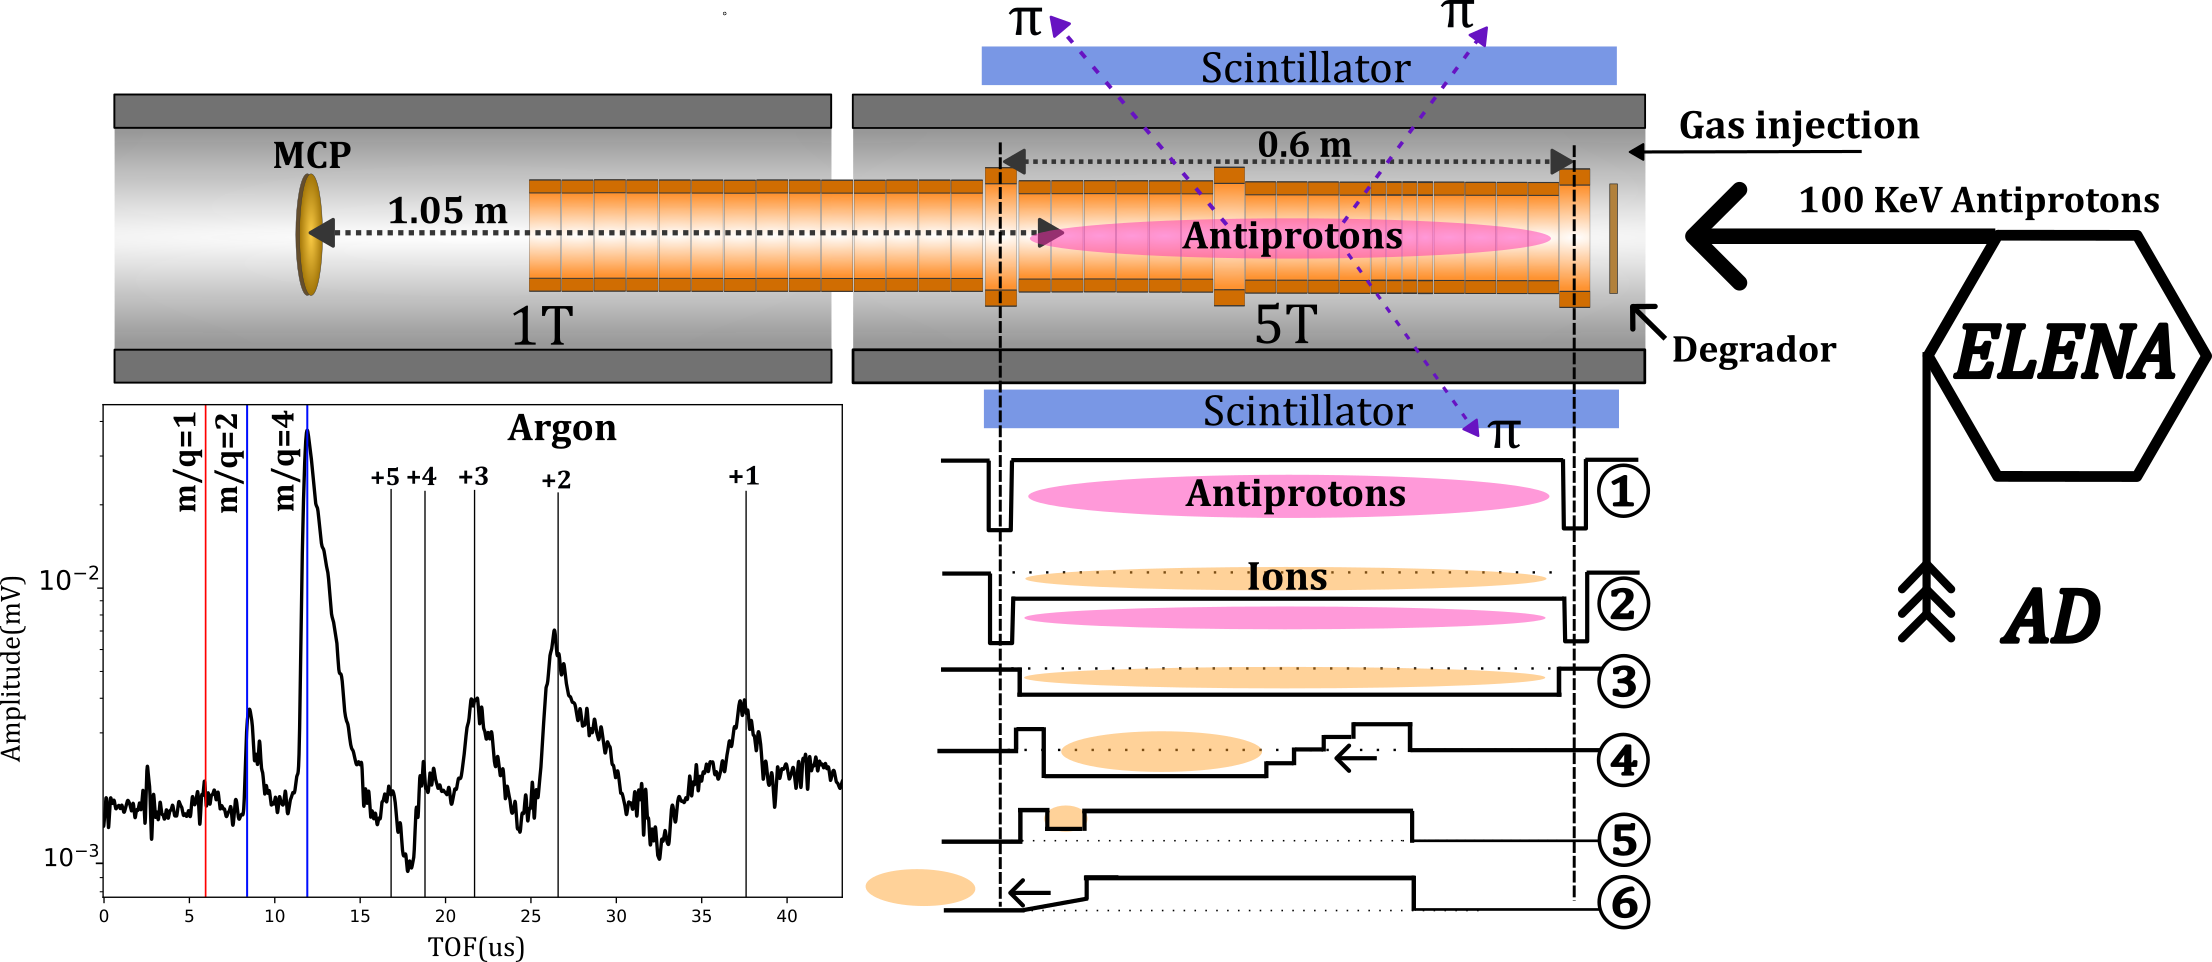
\includegraphics[width=0.8\textwidth, frame]{images/AEGIS_IonTrap.png}
    \end{figure}
    The main goal of \aegis is to measure gravity of atomic antimatter.
\end{frame}

\begin{columnframe}{Background and Motivation}
    \begin{column}{0.5\textwidth}
        \begin{figure}
            \centering
            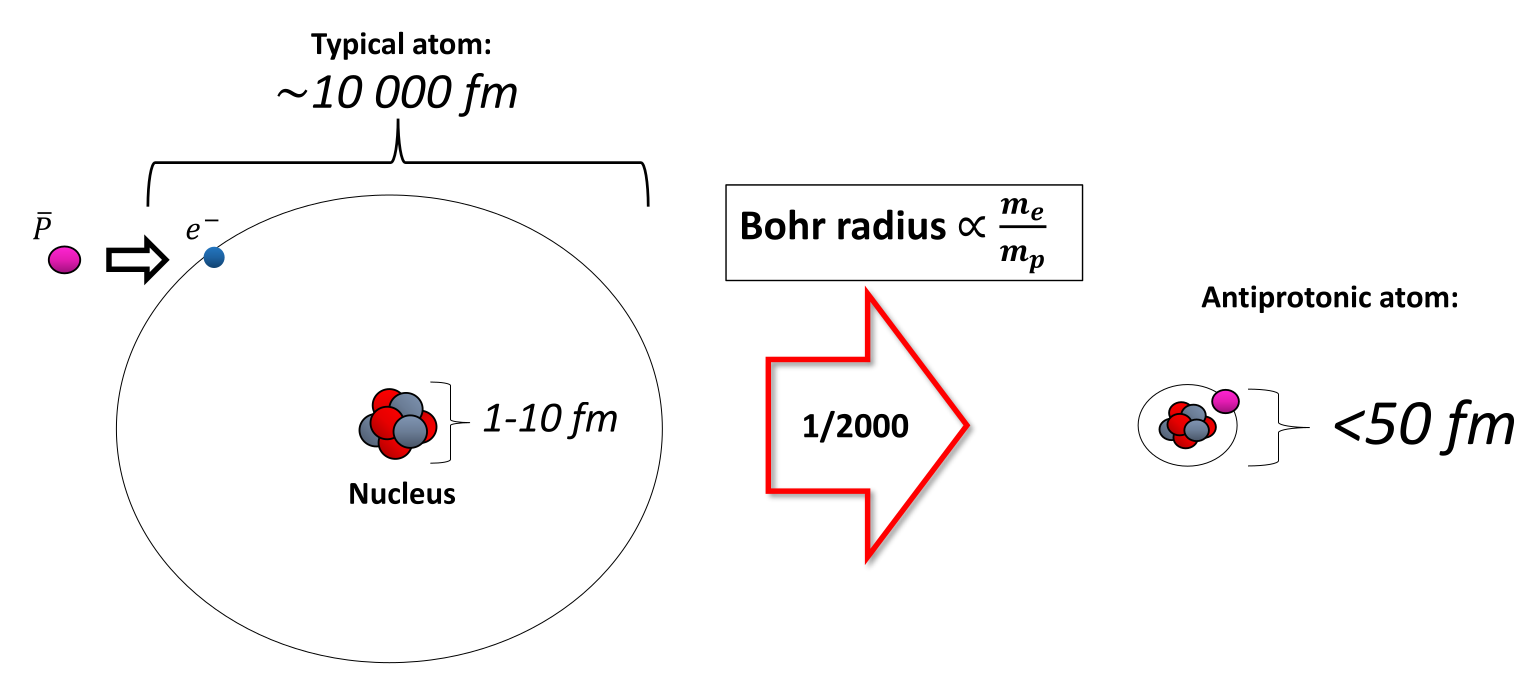
\includegraphics[width=0.95\textwidth, frame]{images/antiprotonic_atom_diagram.png}
        \end{figure}
    \end{column}
    \begin{column}{0.5\textwidth}
        \begin{itemize}
            \item \aegis also studies Antiprotonic Atoms (AA)
            \item AA are formed by exposing low-pressure gas to antiprotons
            \item AA are not stable, they decay fast, emitting radiation
            \item This radiation contains information about the atom
        \end{itemize}
    \end{column}
\end{columnframe}

\begin{columnframe}{The ideal scintillator detector}
    \begin{column}{0.5\textwidth}
        \begin{figure}
            \centering
            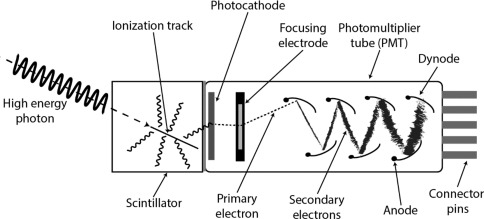
\includegraphics[width=0.95\textwidth]{images/perfect_scintillator.jpg}
        \end{figure}
    \end{column}
    \begin{column}{0.5\textwidth}
        \begin{itemize}
            \item $E_{\text{incident particle}} \longrightarrow N*E_{\gamma - UV}$ (linearly)
            \item Signal height at PMT proportional to $N$
        \end{itemize}
    \end{column}
\end{columnframe}

\begin{columnframe}{Photonis PET detectors}
    \begin{column}{0.5\textwidth}
        \begin{figure}
            \centering
            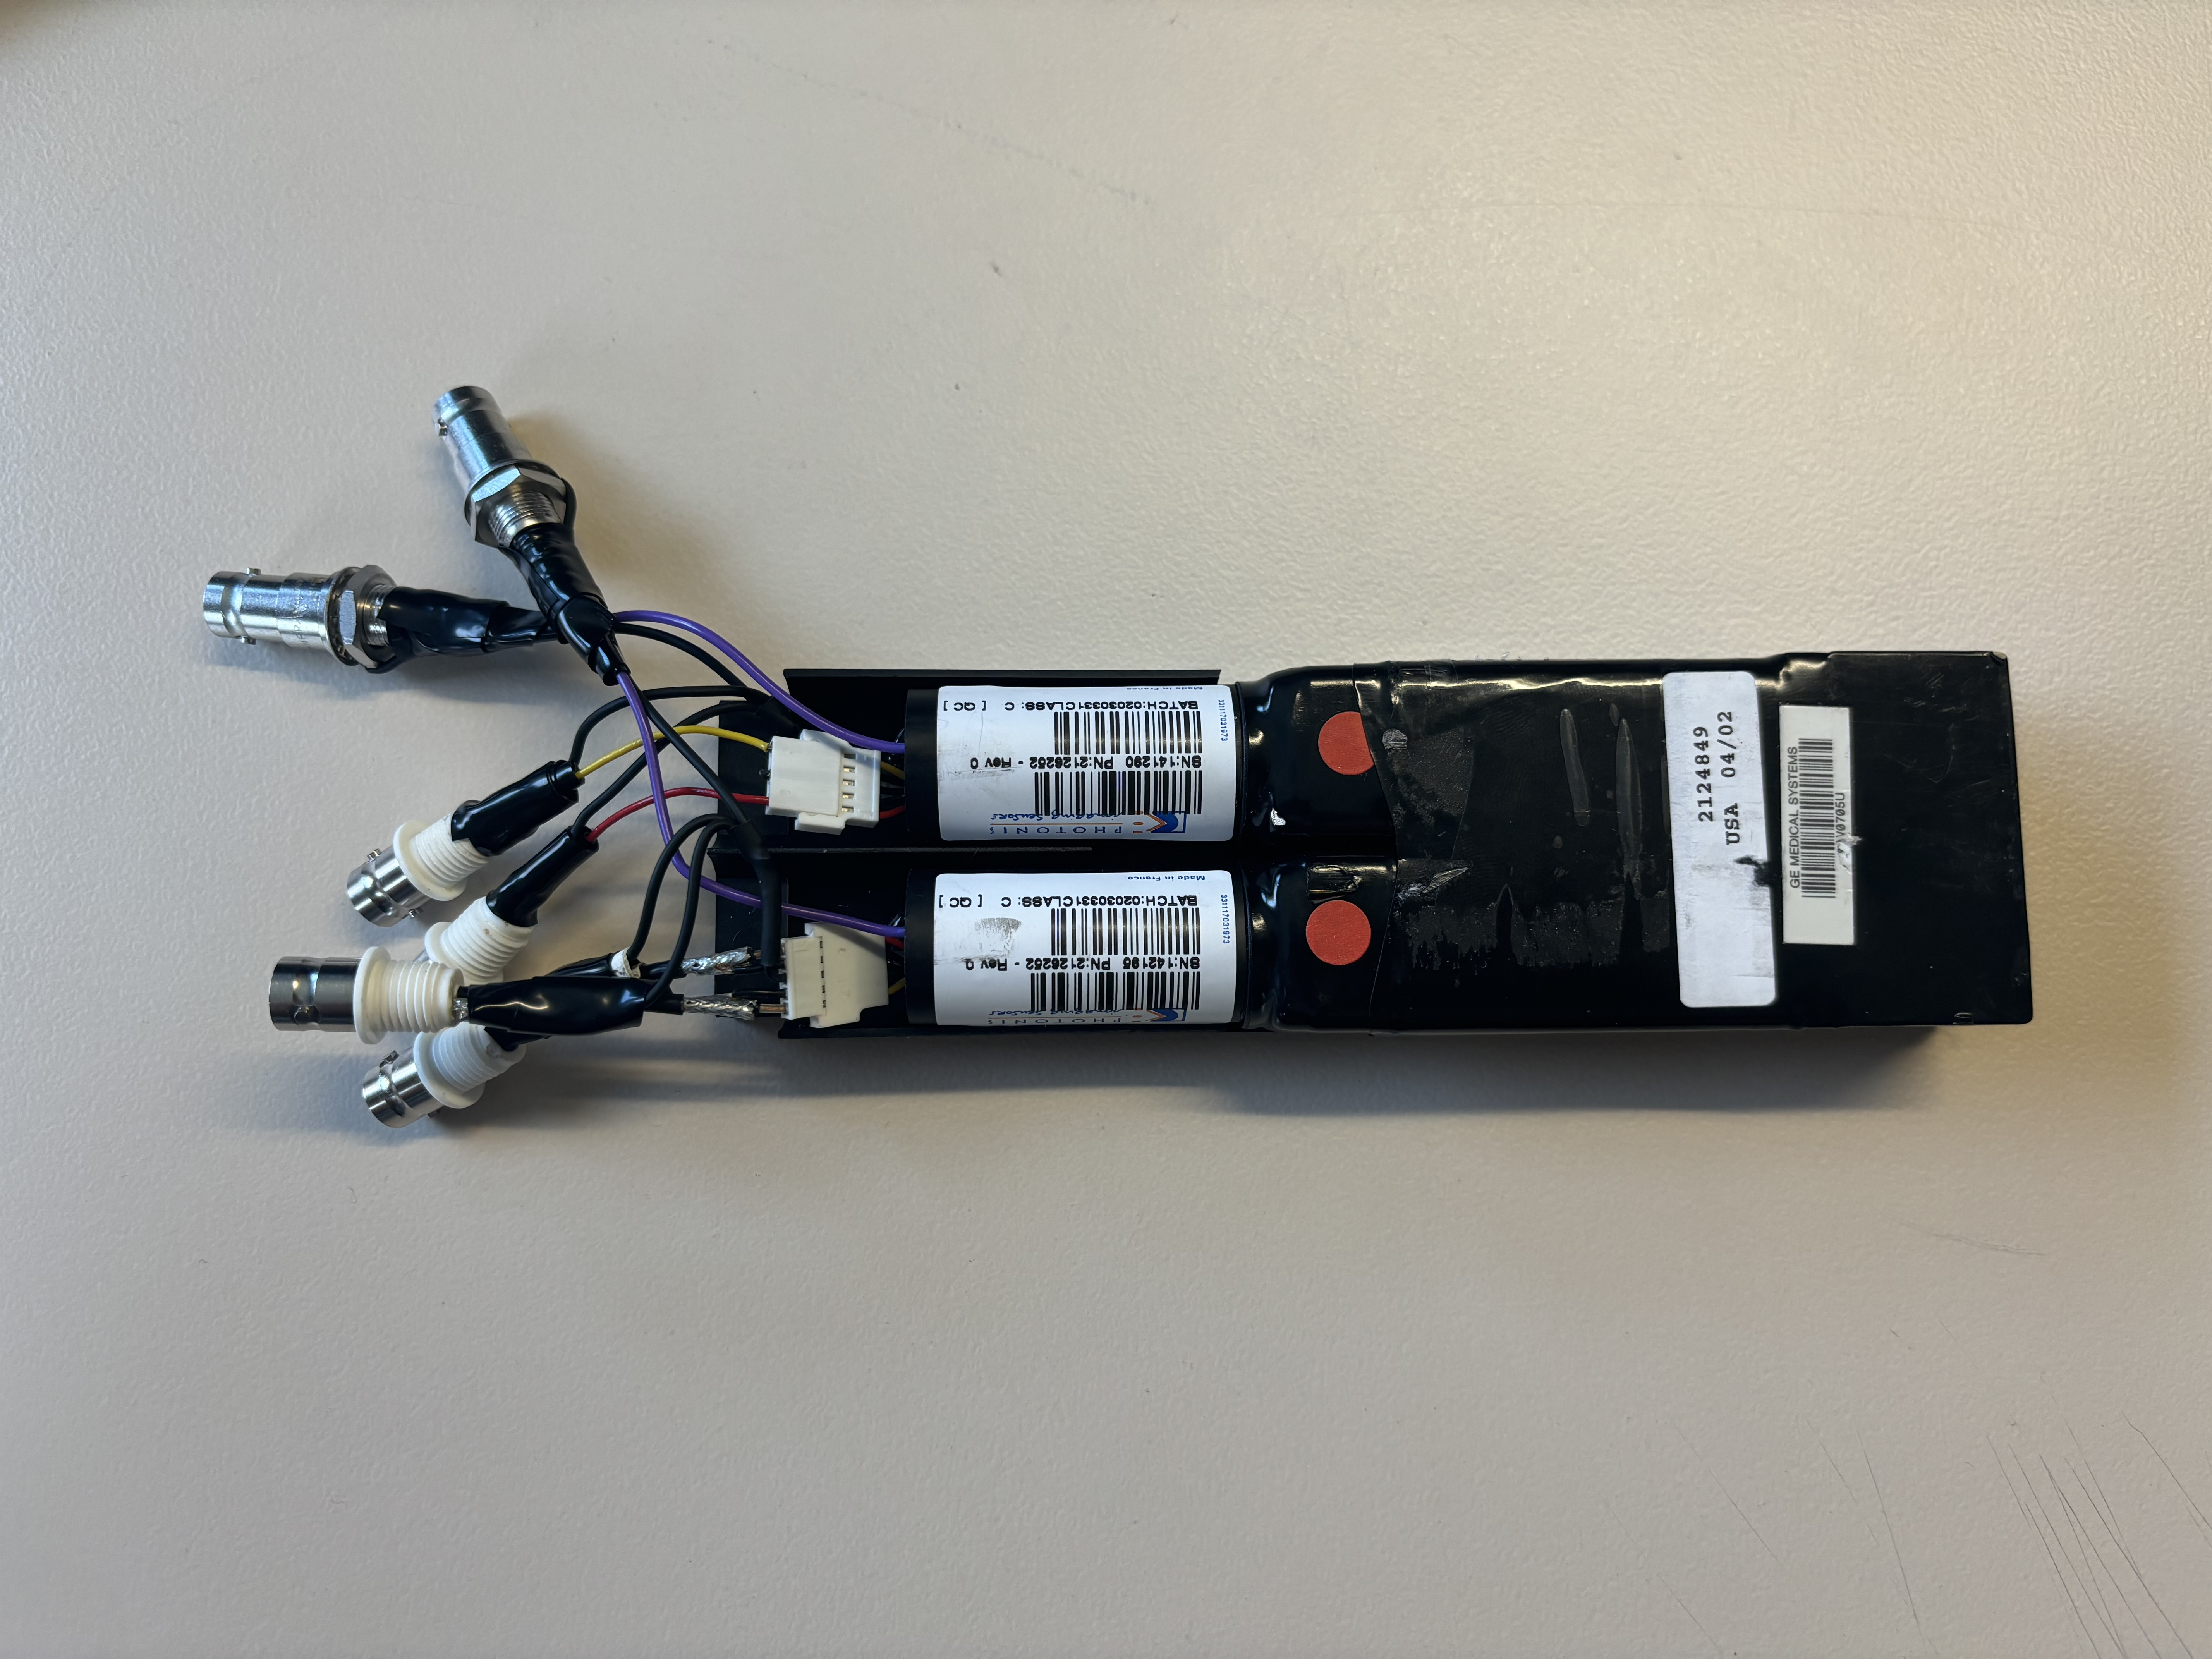
\includegraphics[width=0.9\textwidth, frame]{images/photonis_teardown_1.JPG}
        \end{figure}
    \end{column}
    \begin{column}{0.5\textwidth}
        \begin{itemize}
            \item The detector available is repurposed from a PET scanner
            \item It is a BGO scintillator with a PMT
        \end{itemize}
    \end{column}
\end{columnframe}

\begin{columnframe}{Available radiation sources}
    \begin{column}{0.5\textwidth}
        \begin{figure}
            \centering
            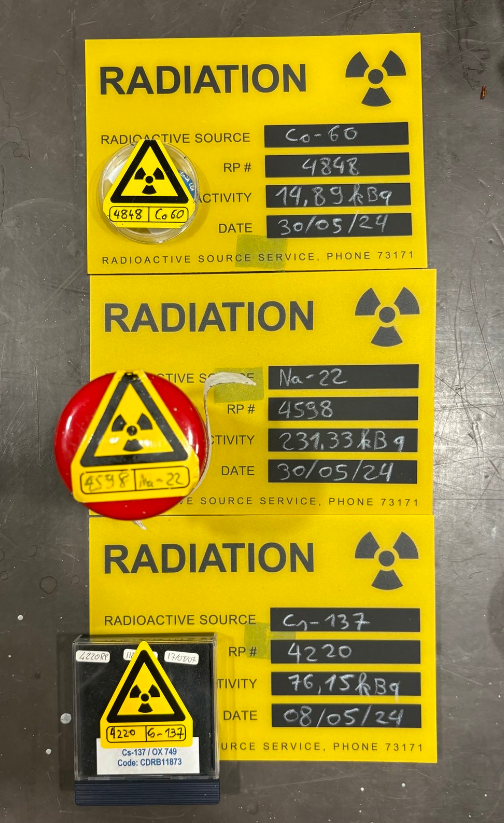
\includegraphics[width=0.6\textwidth, frame]{images/radioactive_sources.png}
        \end{figure}
    \end{column}
    \begin{column}{0.5\textwidth}
        \begin{itemize}
            \item Co-60 - gamma radiation, peaks at 1.17 and 1.33 \MeV
            \item Na-22 - gamma radiation, peaks at 0.511 \MeV and 1.275 \MeV
            \item Cs-137 - gamma radiation, peak at 0.662 \MeV
        \end{itemize}
    \end{column}
\end{columnframe}

\begin{frame}[plain]
    \begin{columns}
        \begin{column}{0.5\textwidth}
            \begin{figure}
                \centering
                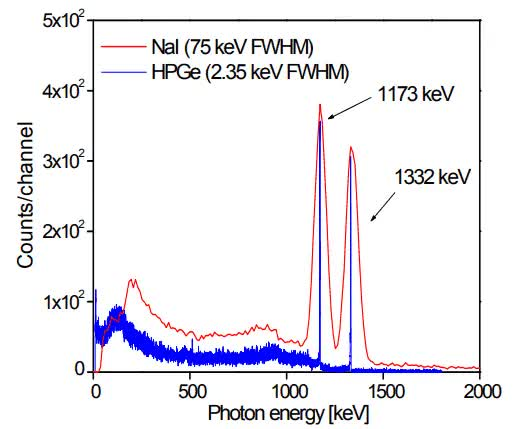
\includegraphics[width=0.8\textwidth, frame]{images/co60_theoretical.jpg}
            \end{figure}
        \end{column}
        \begin{column}{0.5\textwidth}
            \begin{figure}
                \centering
                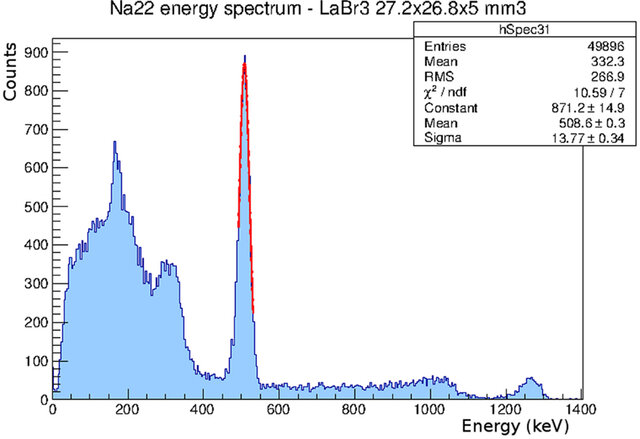
\includegraphics[width=0.99\textwidth, frame]{images/na22_theoretical.jpg}
            \end{figure}
        \end{column}
    \end{columns}
    \begin{columns}
        \begin{column}{0.5\textwidth}
            \begin{figure}
                \centering
                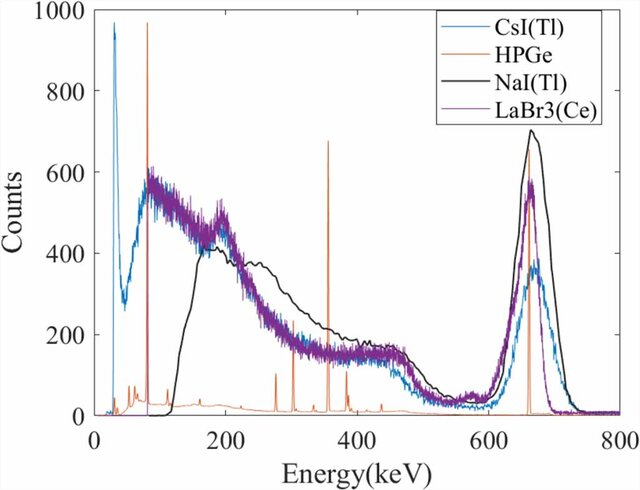
\includegraphics[width=0.8\textwidth, frame]{images/cs137_theoretical.jpg}
            \end{figure}
        \end{column}
        \begin{column}{0.5\textwidth}
            \imagesource{Gabriela Llosá, Trovato Marco, John Barrio, Ane Etxebeste, Enrique Muñoz, Carlos Lacasta, Josep Oliver,
                Magdalena Rafecas, Carles Solaz, and Paola Solevi. First images of a three-layer compton telescope
                prototype for treatment monitoring in hadron therapy. Frontiers in Oncology, 6, 02 2016.}
            \vspace{0.3cm}

            \imagesource{nuclear-power.com.
                Spectroscopy using germanium semiconductor – hpge.
                https://www.nuclear-power.com/nuclear-engineering/
                radiation-detection/gamma-spectroscopy/
                spectroscopy-using-germanium-semiconductor-hpge/, 2025. Accessed: 2025-05-07.}
            \vspace{0.3cm}

            \imagesource{Kajal Kumari and Mayank Goswami. Relative estimation of scattering noise and electronic noise of a
                radiation detector. Measurement Science and Technology, 34, 08 2023.}
        \end{column}
    \end{columns}
\end{frame}

\begin{columnframe}{Teardown}
    \begin{column}{0.5\textwidth}
        \begin{figure}
            \centering
            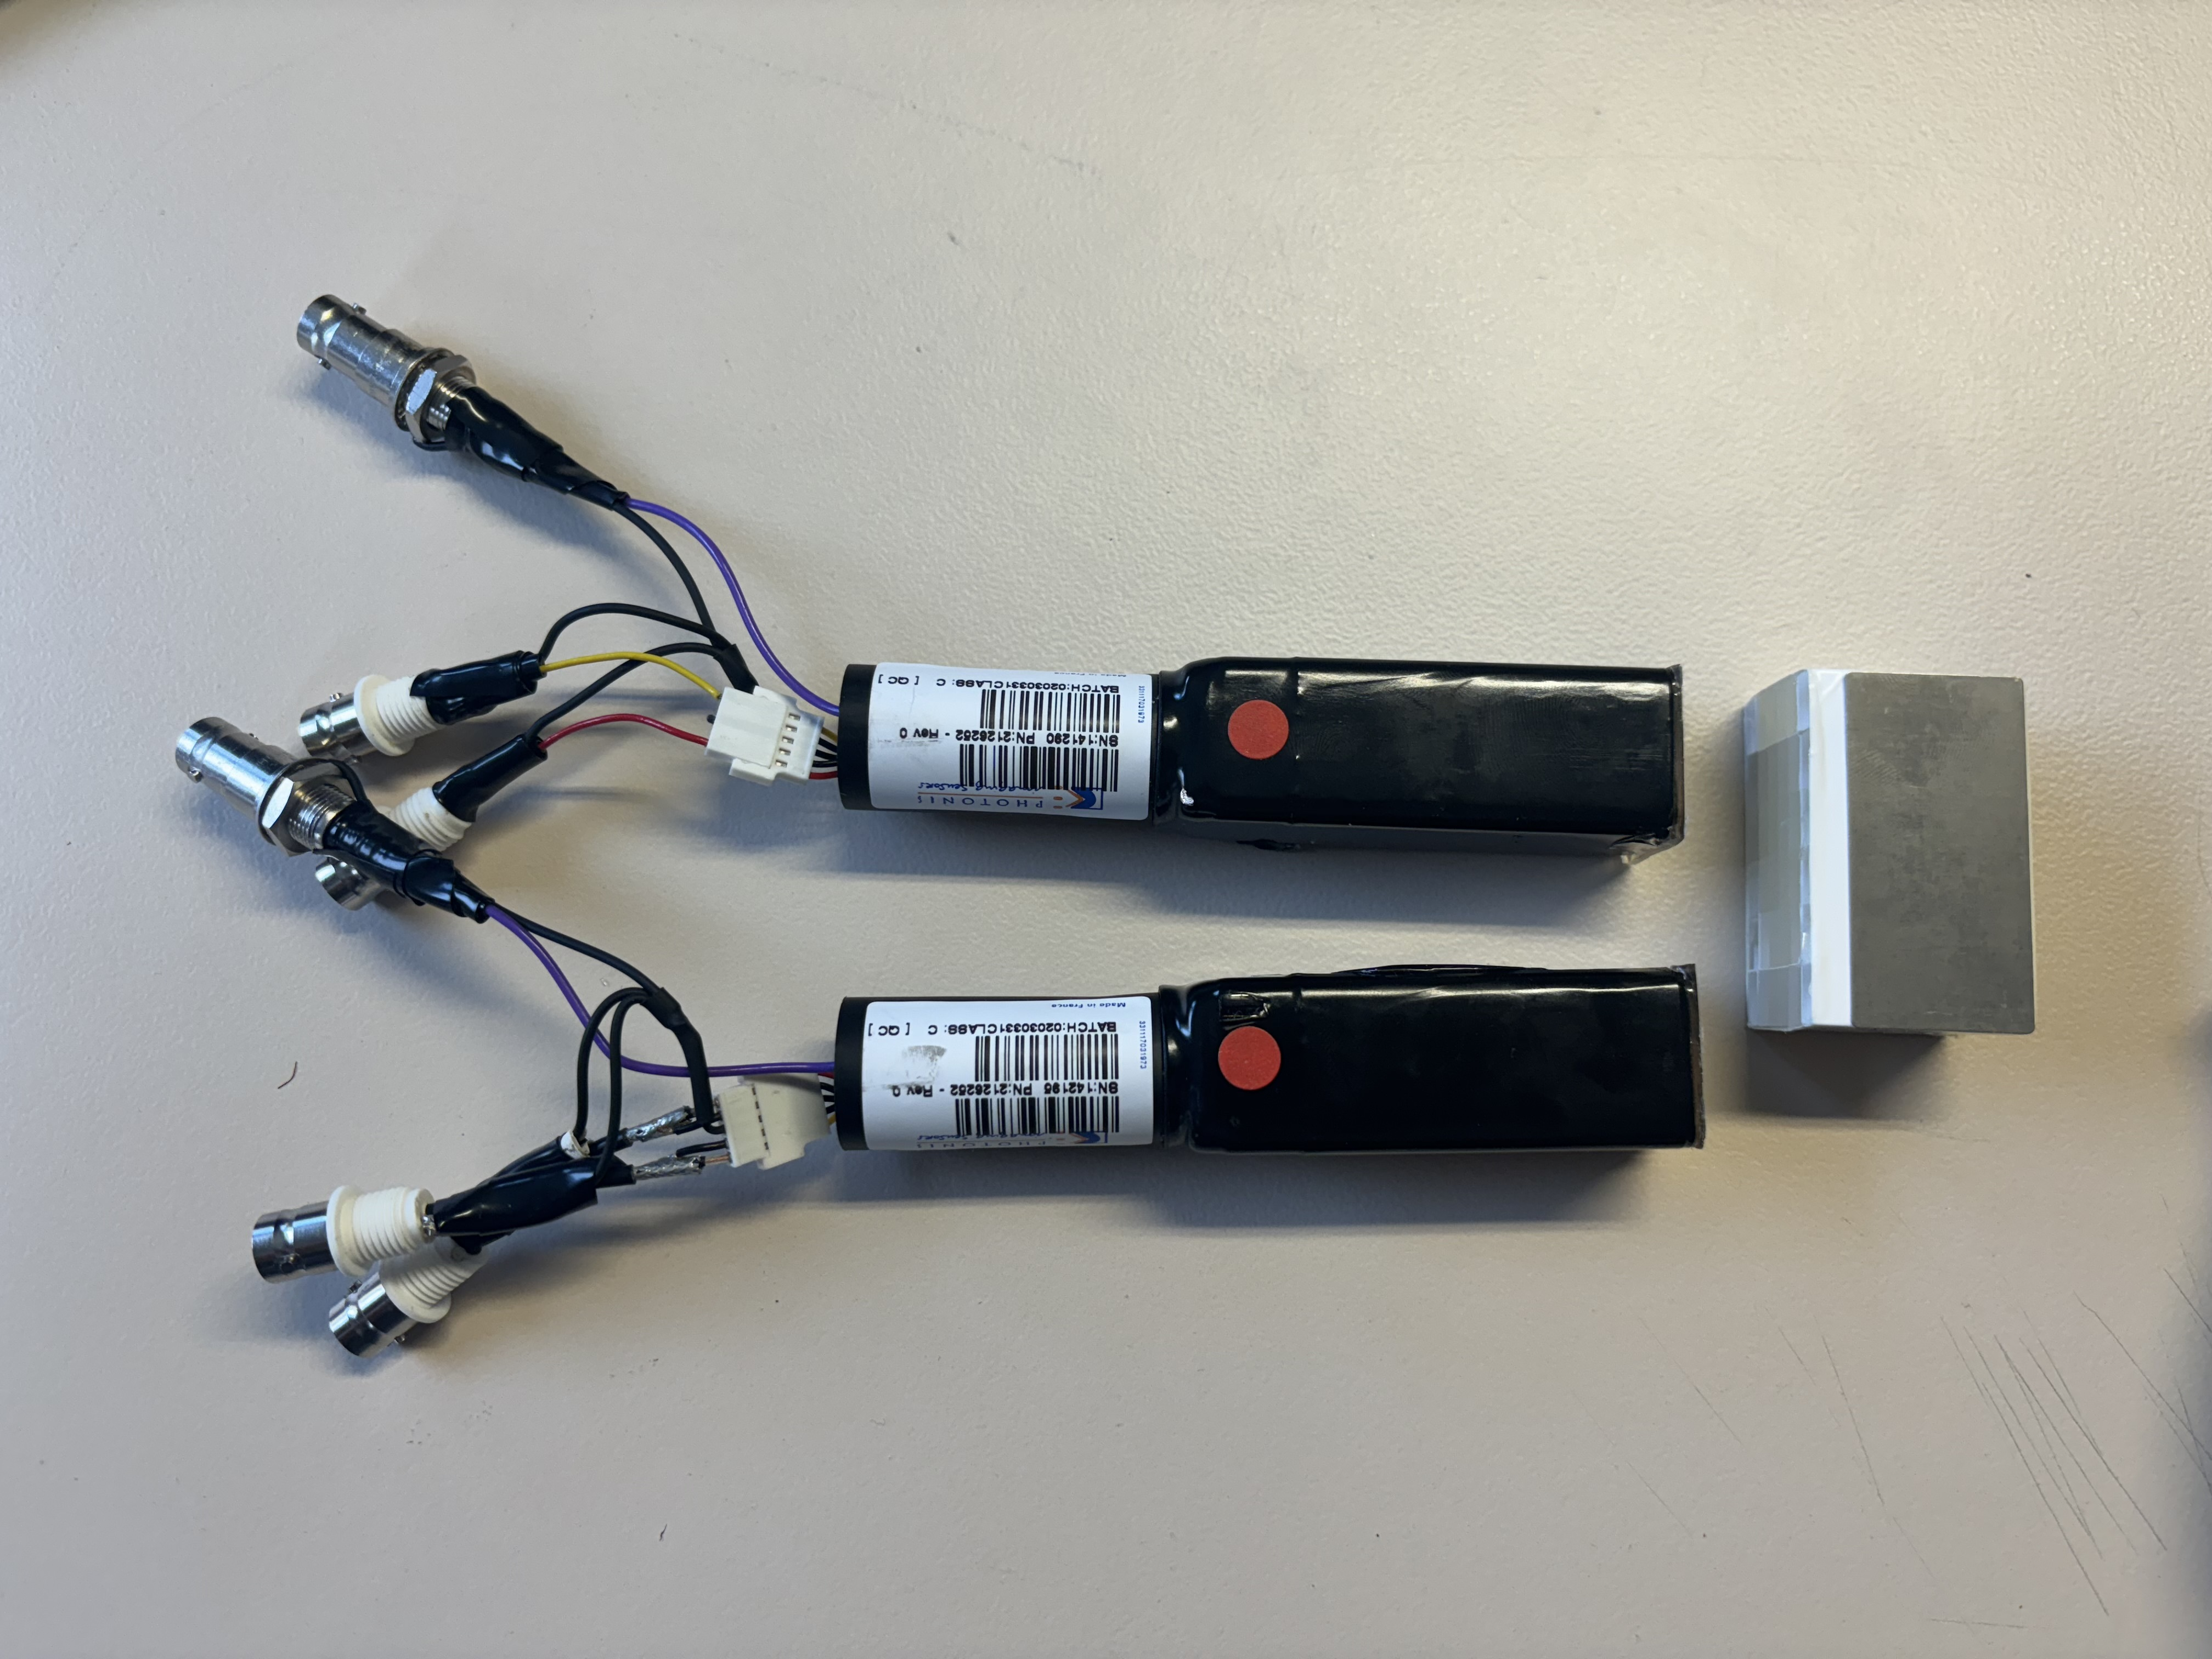
\includegraphics[width=0.6\textwidth, frame]{images/photonis_teardown_4.JPG}
            % direction: trim=left bottom right top
            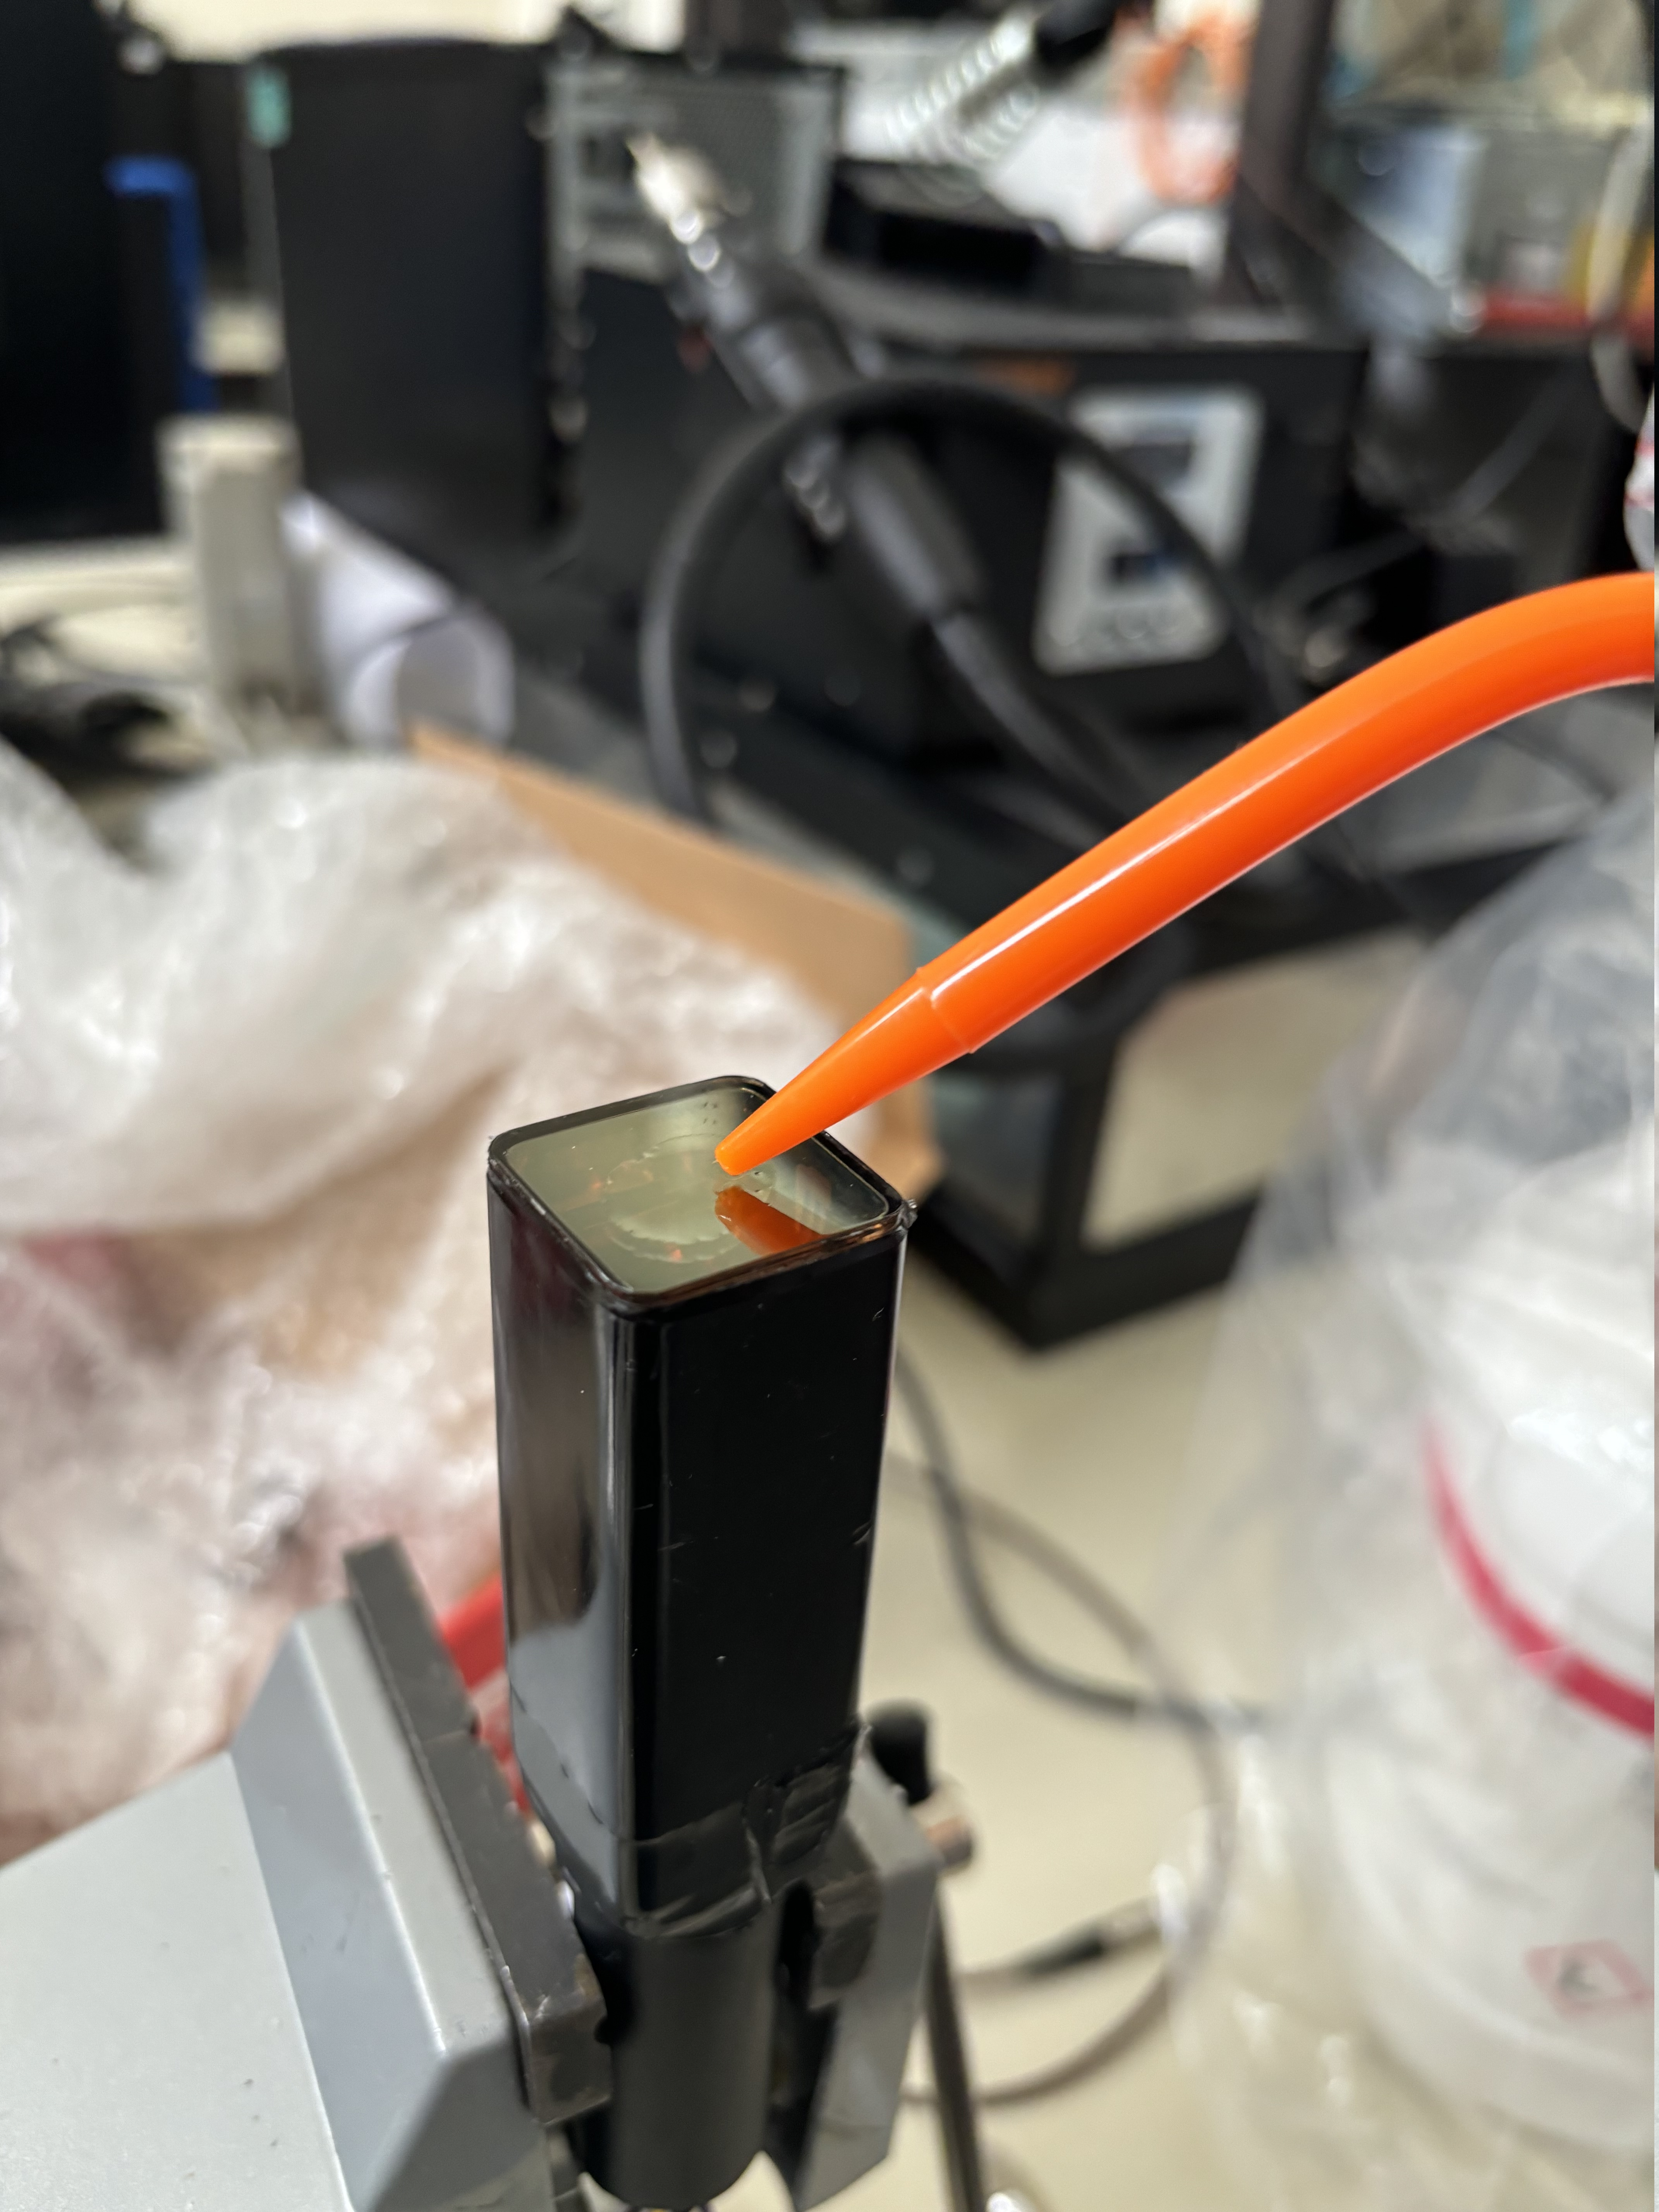
\includegraphics[trim=0 200 0 1800, clip, width=0.6\textwidth, frame]{images/PMT_iso_wipe.JPG}
        \end{figure}
    \end{column}
    \begin{column}{0.5\textwidth}
        \begin{figure}
            \centering
            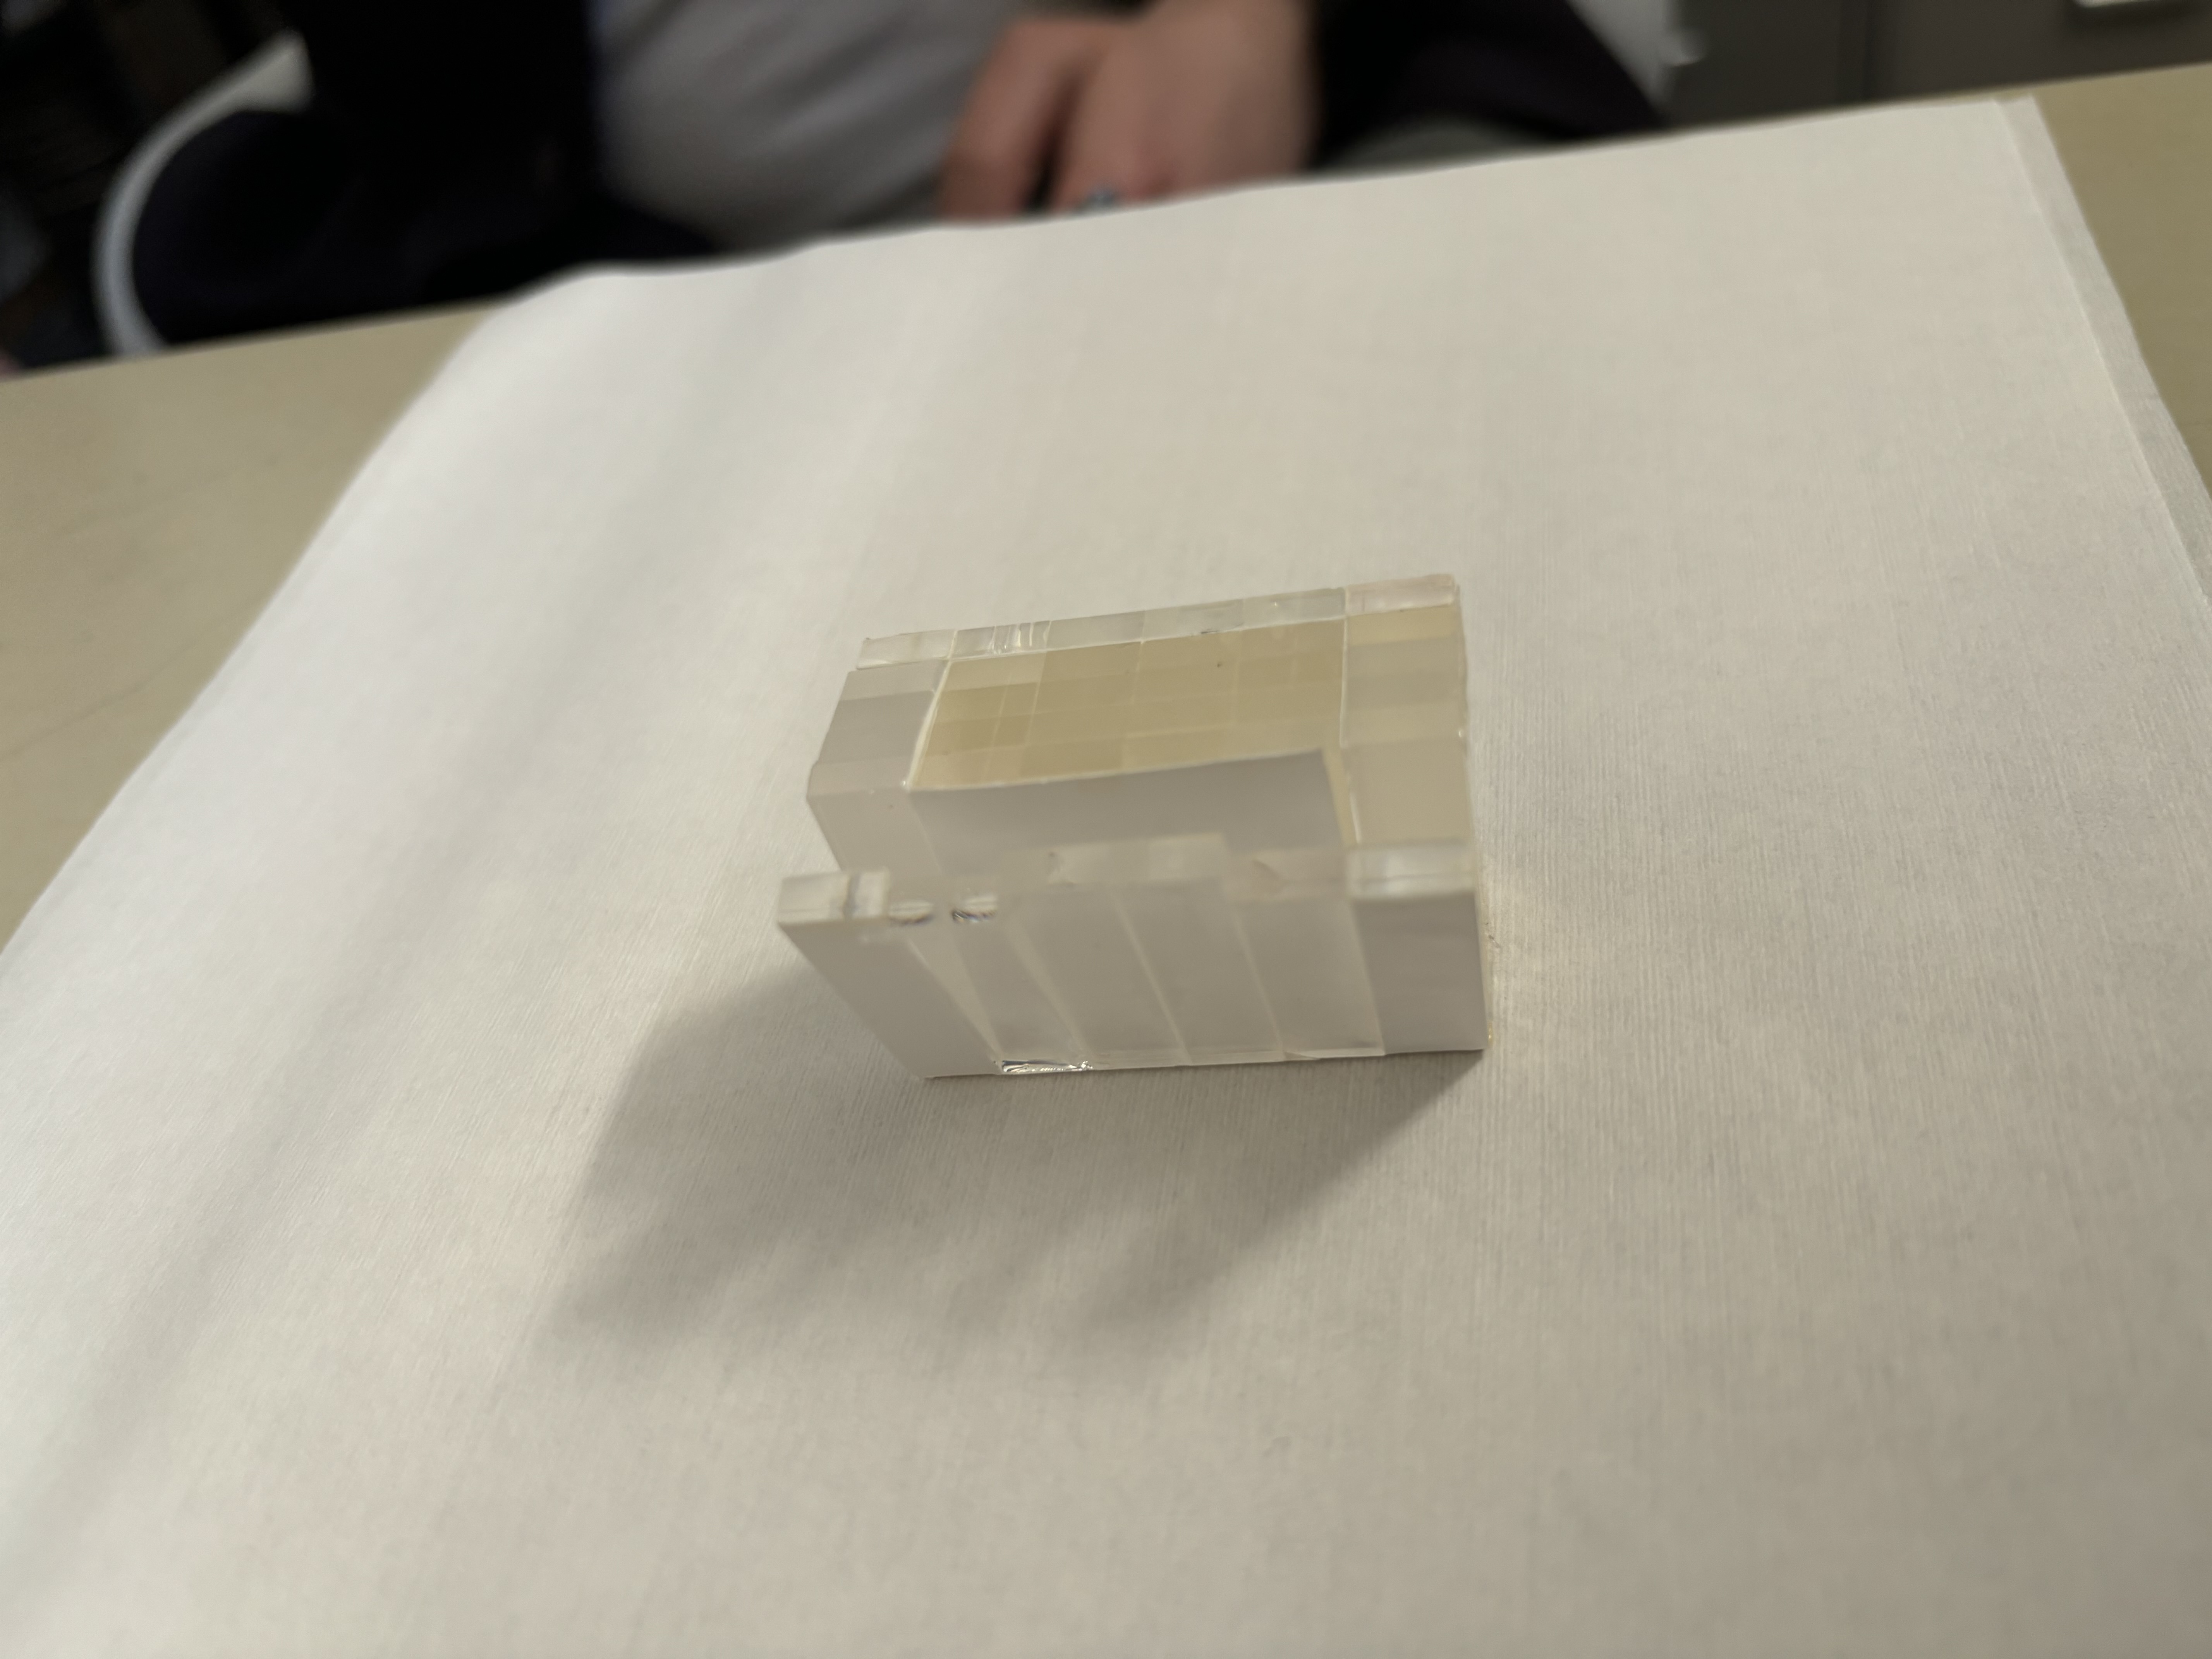
\includegraphics[width=0.6\textwidth, frame]{images/crystals_pack_2.JPG}
        \end{figure}
        \begin{itemize}
            \item The initial performance of the module was subpar
            \item The detector was disassembled for component-level analysis
        \end{itemize}
    \end{column}
\end{columnframe}

\begin{frame}{Teardown - Broken Stripped PMT}
    \begin{figure}
        \centering
        \includegraphics[trim=0 120 0 70, clip, width=0.9\textwidth, frame]{images/stripped_pmt_3_annotated.png}
    \end{figure}
\end{frame}

% \begin{columnframe}{}
%     \begin{column}{0.5\textwidth}
%     \end{column}
%     \begin{column}{0.5\textwidth}
%     \end{column}
% \end{columnframe}

\begin{columnframe}{PMT noise to signal ratio}
    \begin{column}{0.5\textwidth}
        \begin{figure}
            \centering
            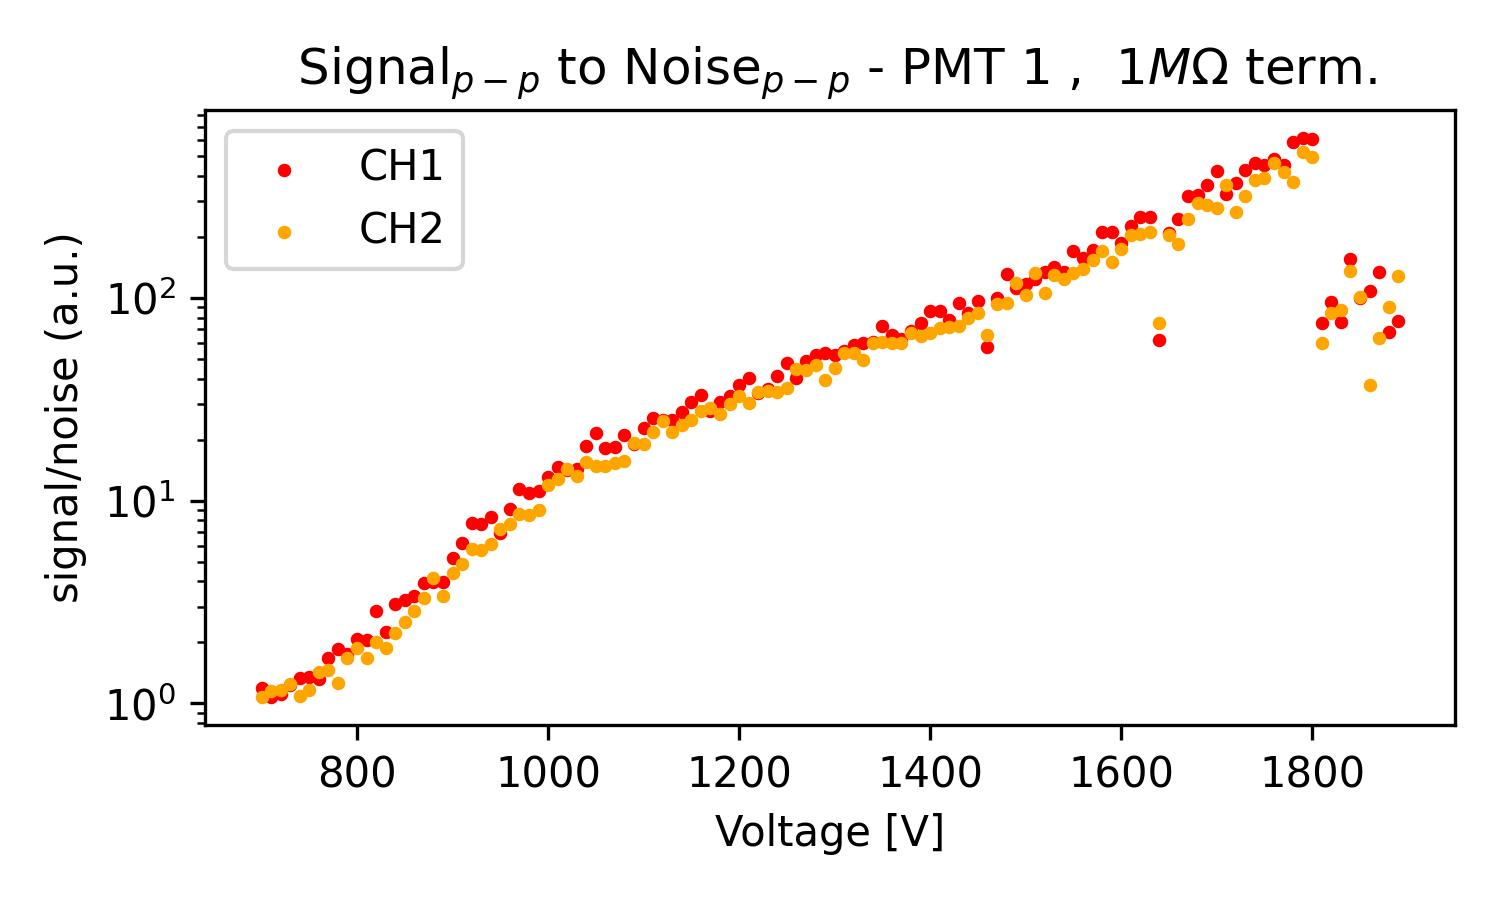
\includegraphics[width=0.9\textwidth, frame]{images/sigp2p_to_noisep2p.jpg}
        \end{figure}
    \end{column}
    \begin{column}{0.5\textwidth}
        \begin{itemize}
            \item The noise of the PMT was measured as a function of bias voltage
            \item The signal height was measured separately
            \item The noise to signal ratio was calculated
            \item Optimal bias voltage was found to be 1450 \si{\volt}
        \end{itemize}
    \end{column}
\end{columnframe}


\begin{frame}{Measuring Time Characteristics}
    \begin{figure}
        \centering
        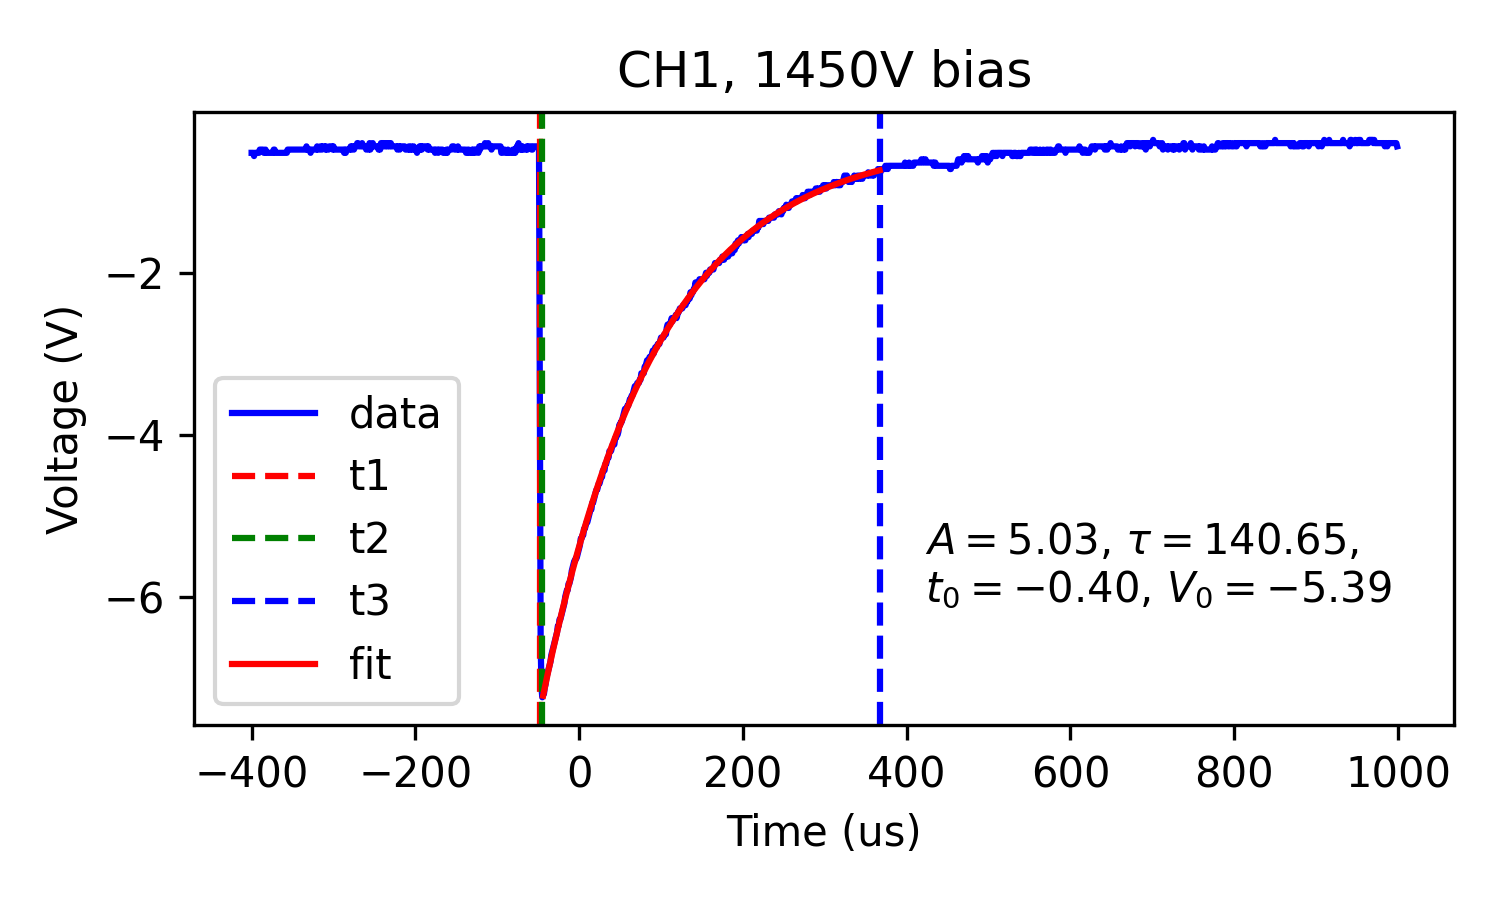
\includegraphics[width=0.7\textwidth]{images/example_time_fitting.png}
    \end{figure}
\end{frame}

\begin{columnframe}{Signal/Bias Voltage Time Characteristics}
    \begin{column}{0.5\textwidth}
        \begin{figure}
            \centering
            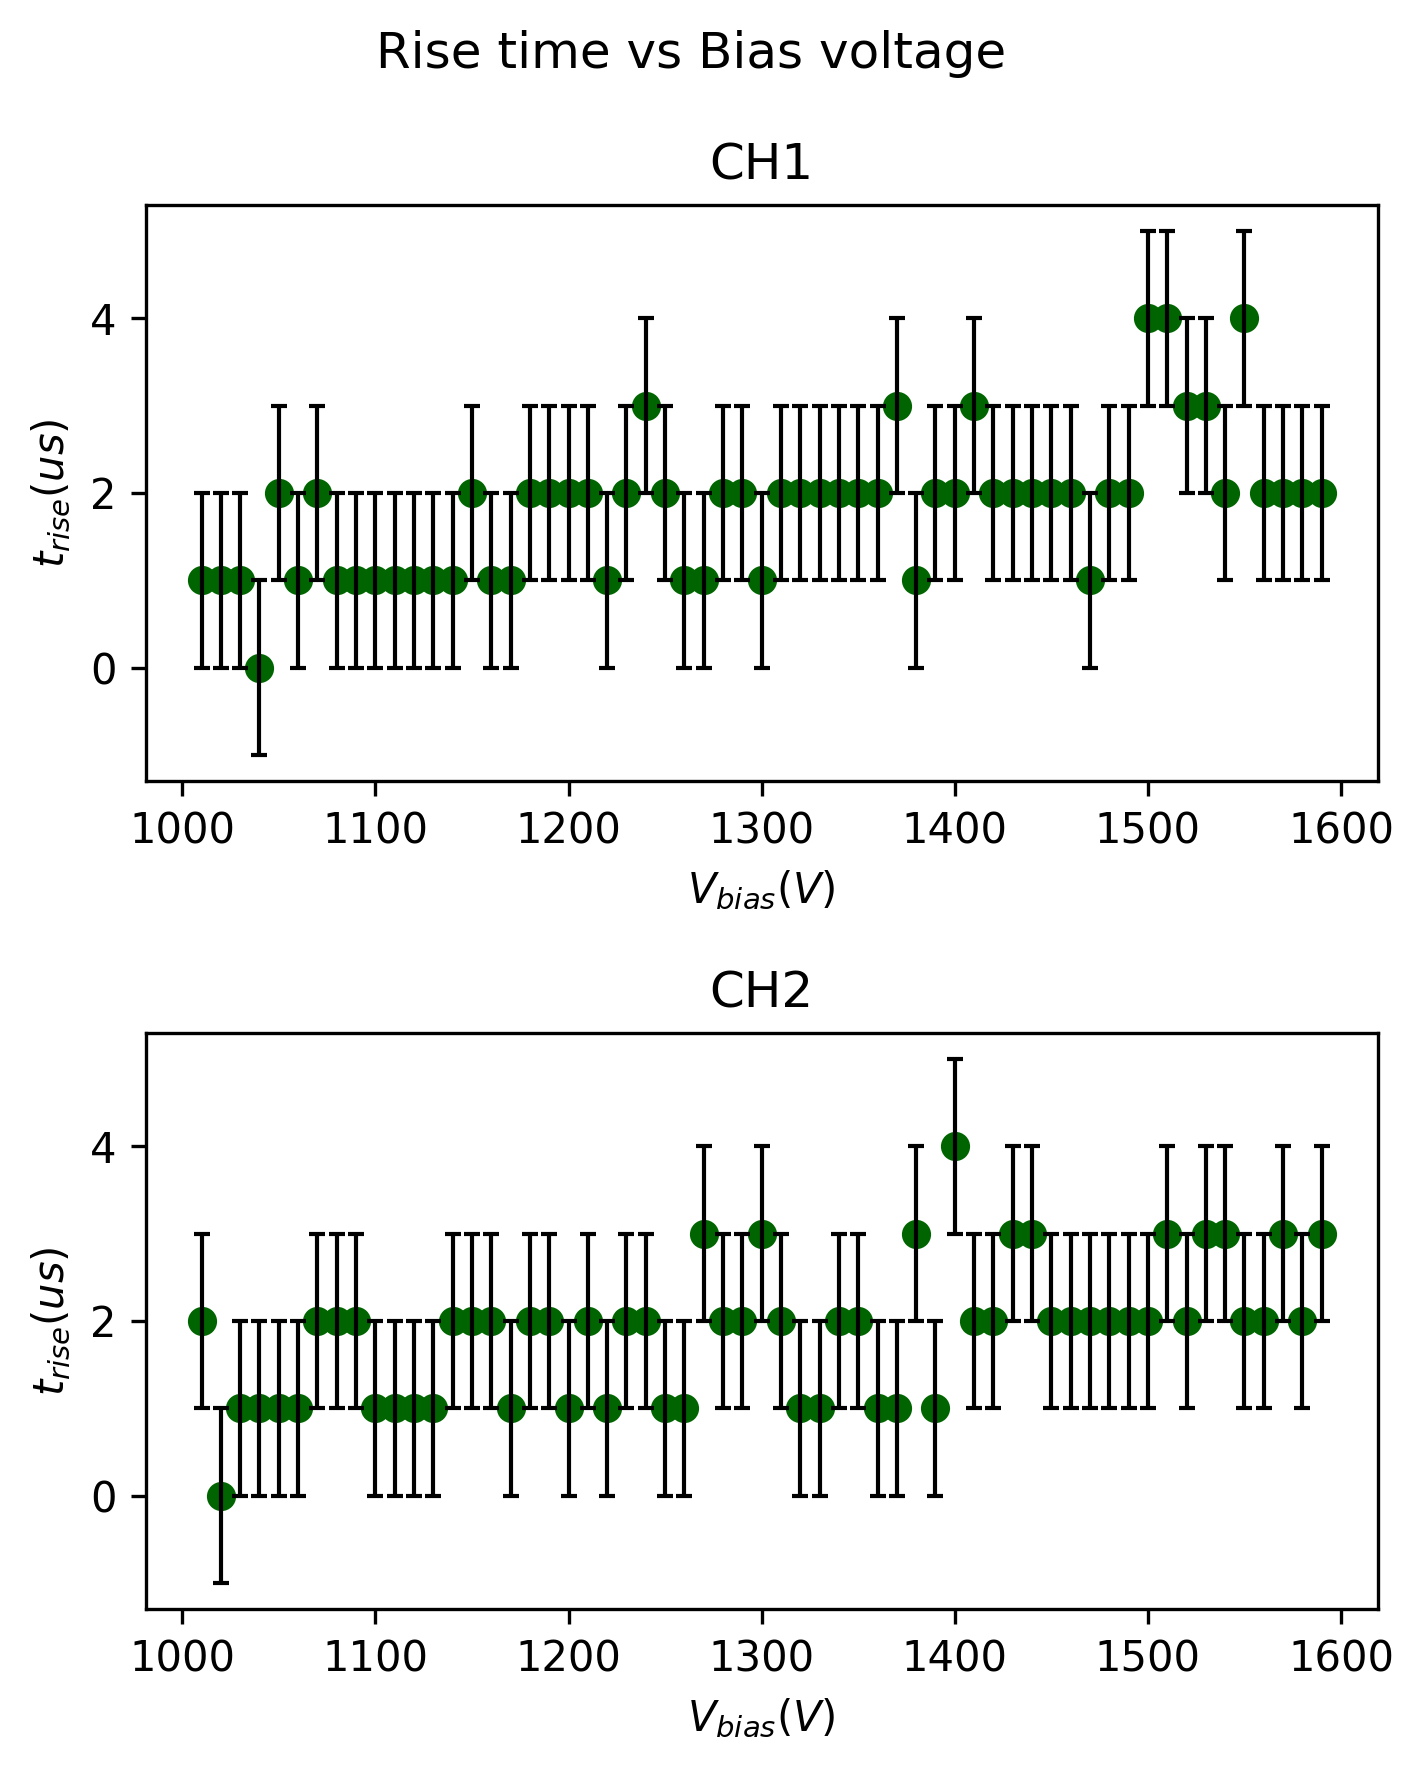
\includegraphics[width=0.8\textwidth, frame]{images/rise_times_bias.png}
        \end{figure}
    \end{column}
    \begin{column}{0.5\textwidth}
        \begin{figure}
            \centering
            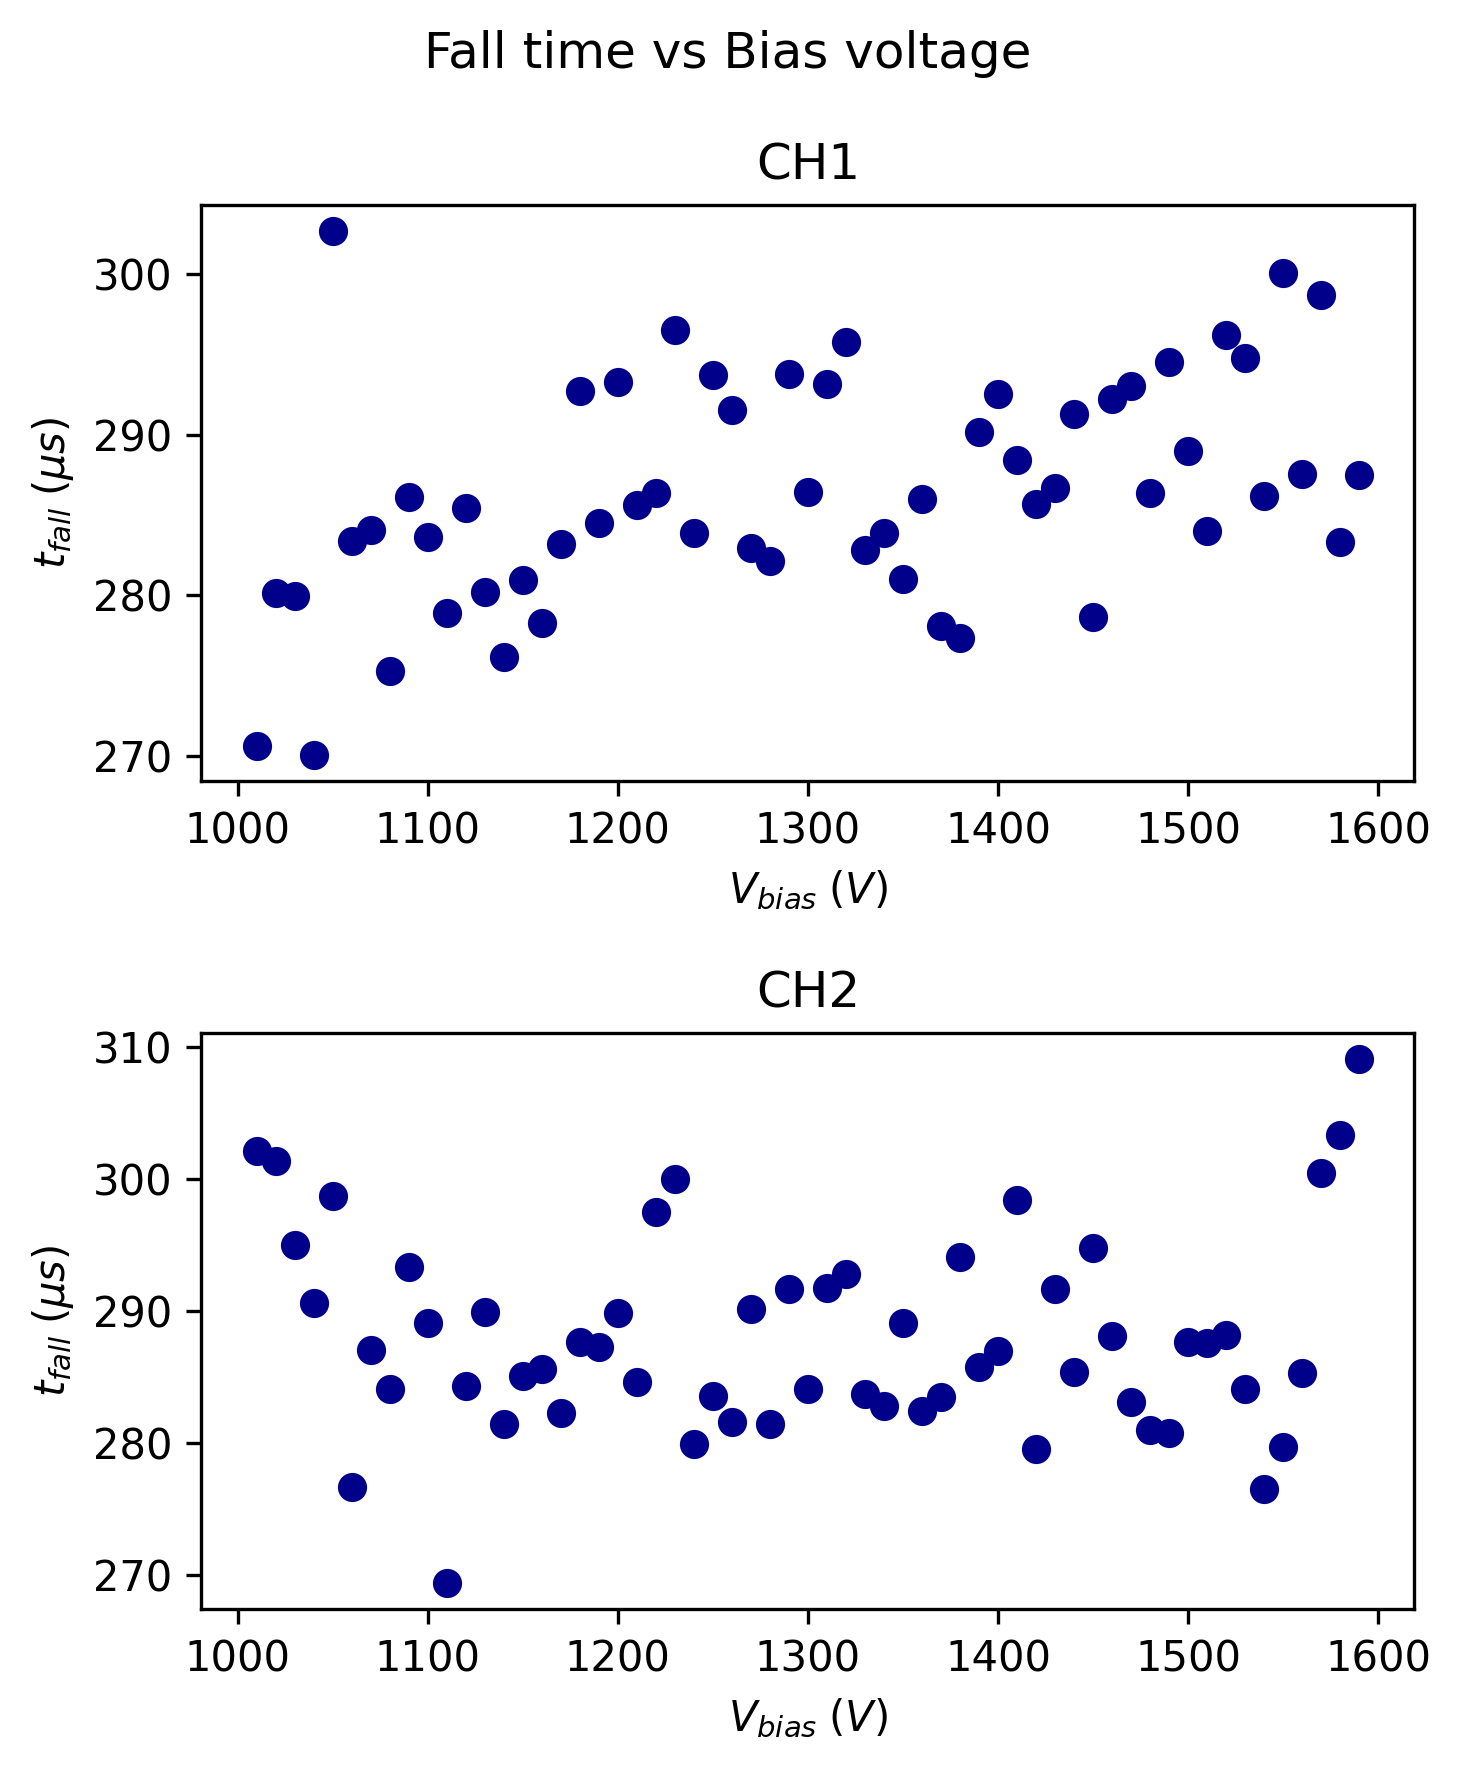
\includegraphics[width=0.8\textwidth, frame]{images/fall_times_bias.png}
        \end{figure}
    \end{column}
\end{columnframe}

\begin{columnframe}{Signal Light Intensity Time Characteristics}
    \begin{column}{0.5\textwidth}
        \begin{figure}
            \centering
            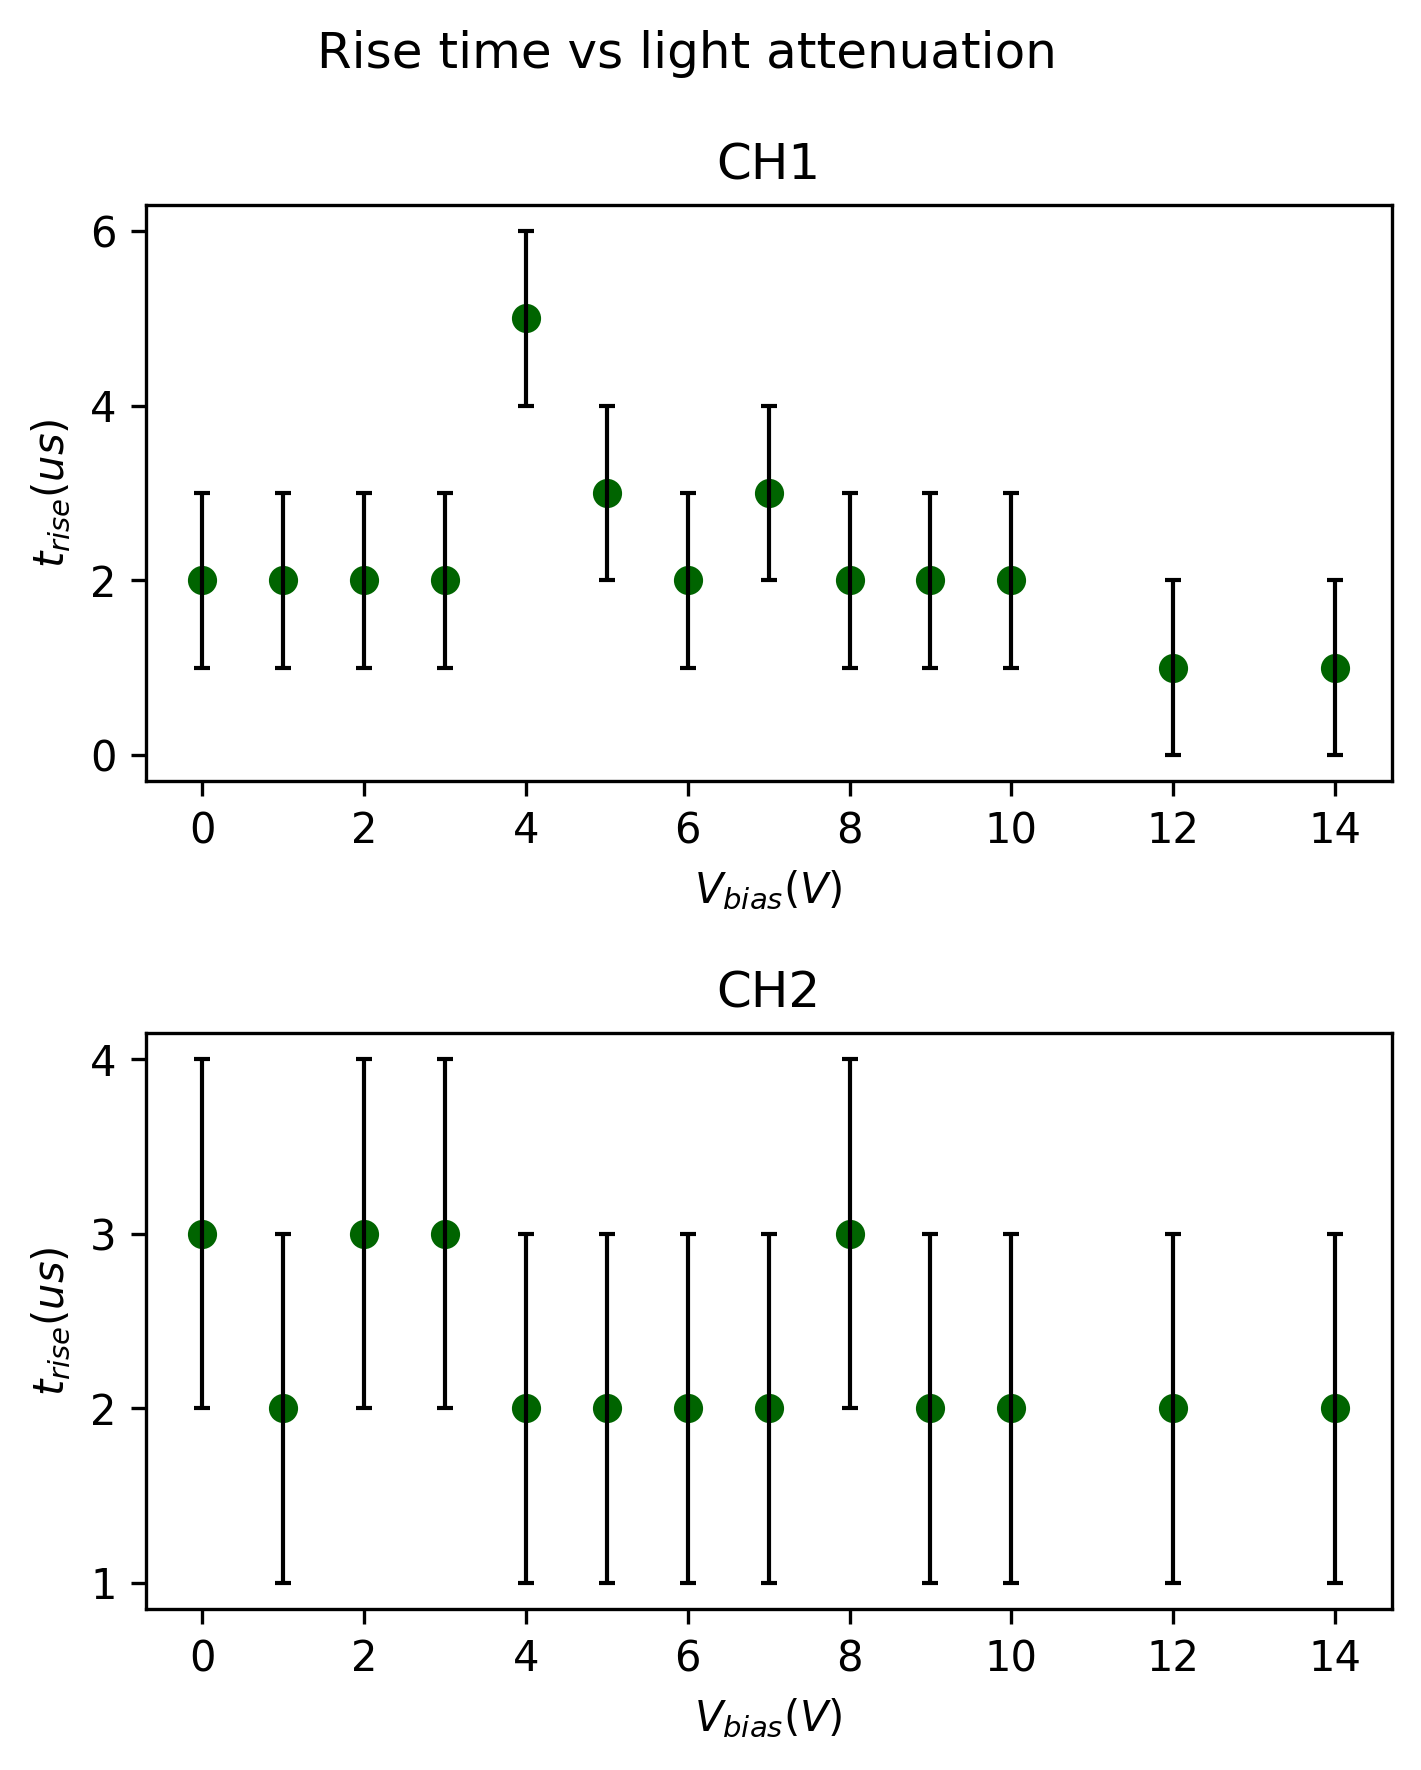
\includegraphics[width=0.8\textwidth, frame]{images/rise_times_att.png}
        \end{figure}
    \end{column}
    \begin{column}{0.5\textwidth}
        \begin{figure}
            \centering
            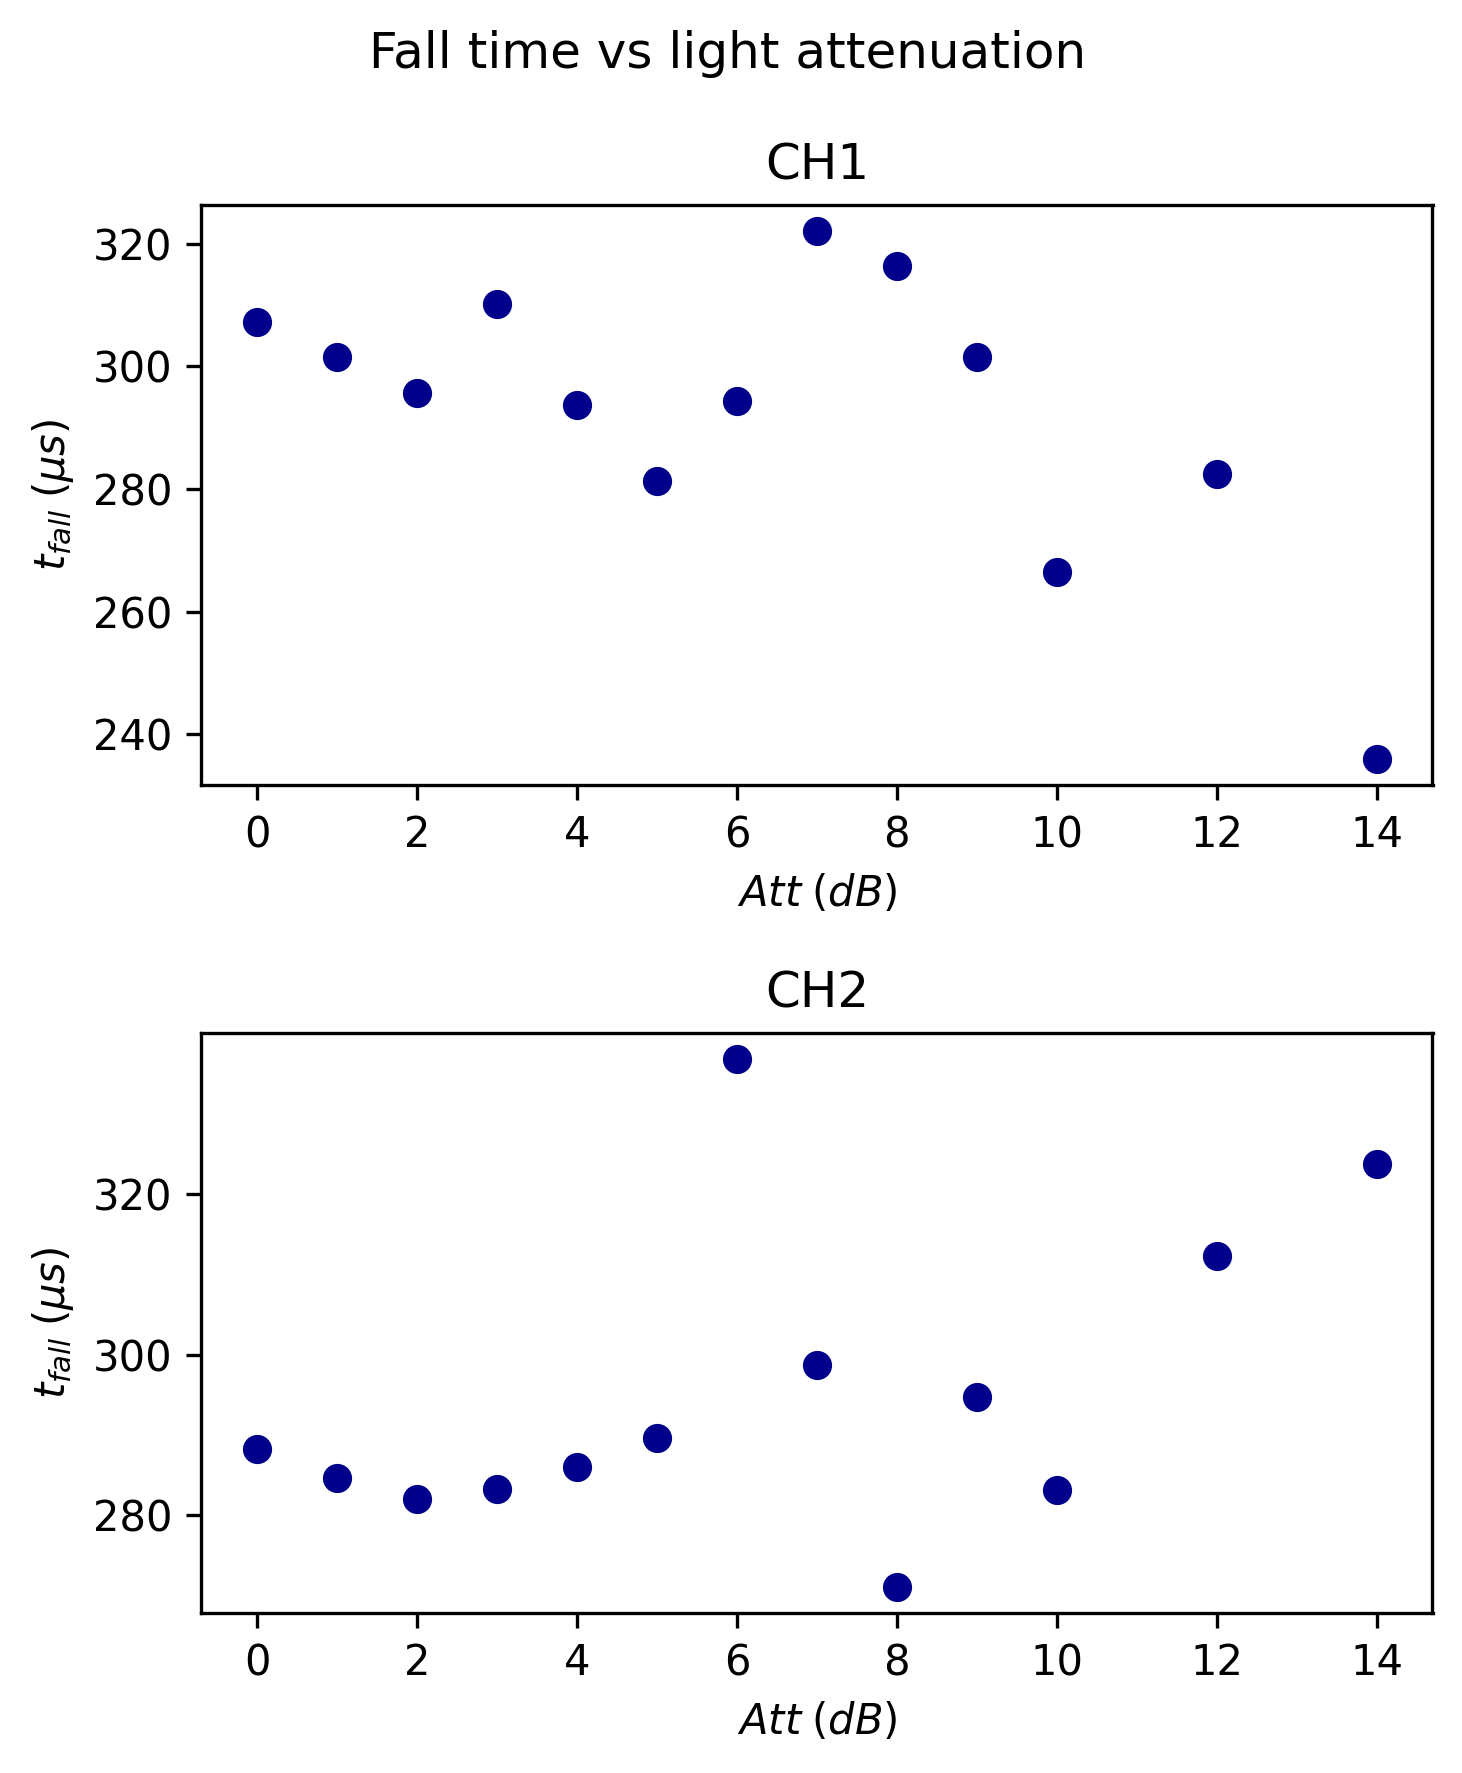
\includegraphics[width=0.8\textwidth, frame]{images/fall_times_att.png}
        \end{figure}
    \end{column}
\end{columnframe}

\begin{columnframe}{PMT Spectroscopy Setup}
    \begin{column}{0.5\textwidth}
        \begin{figure}
            \centering
            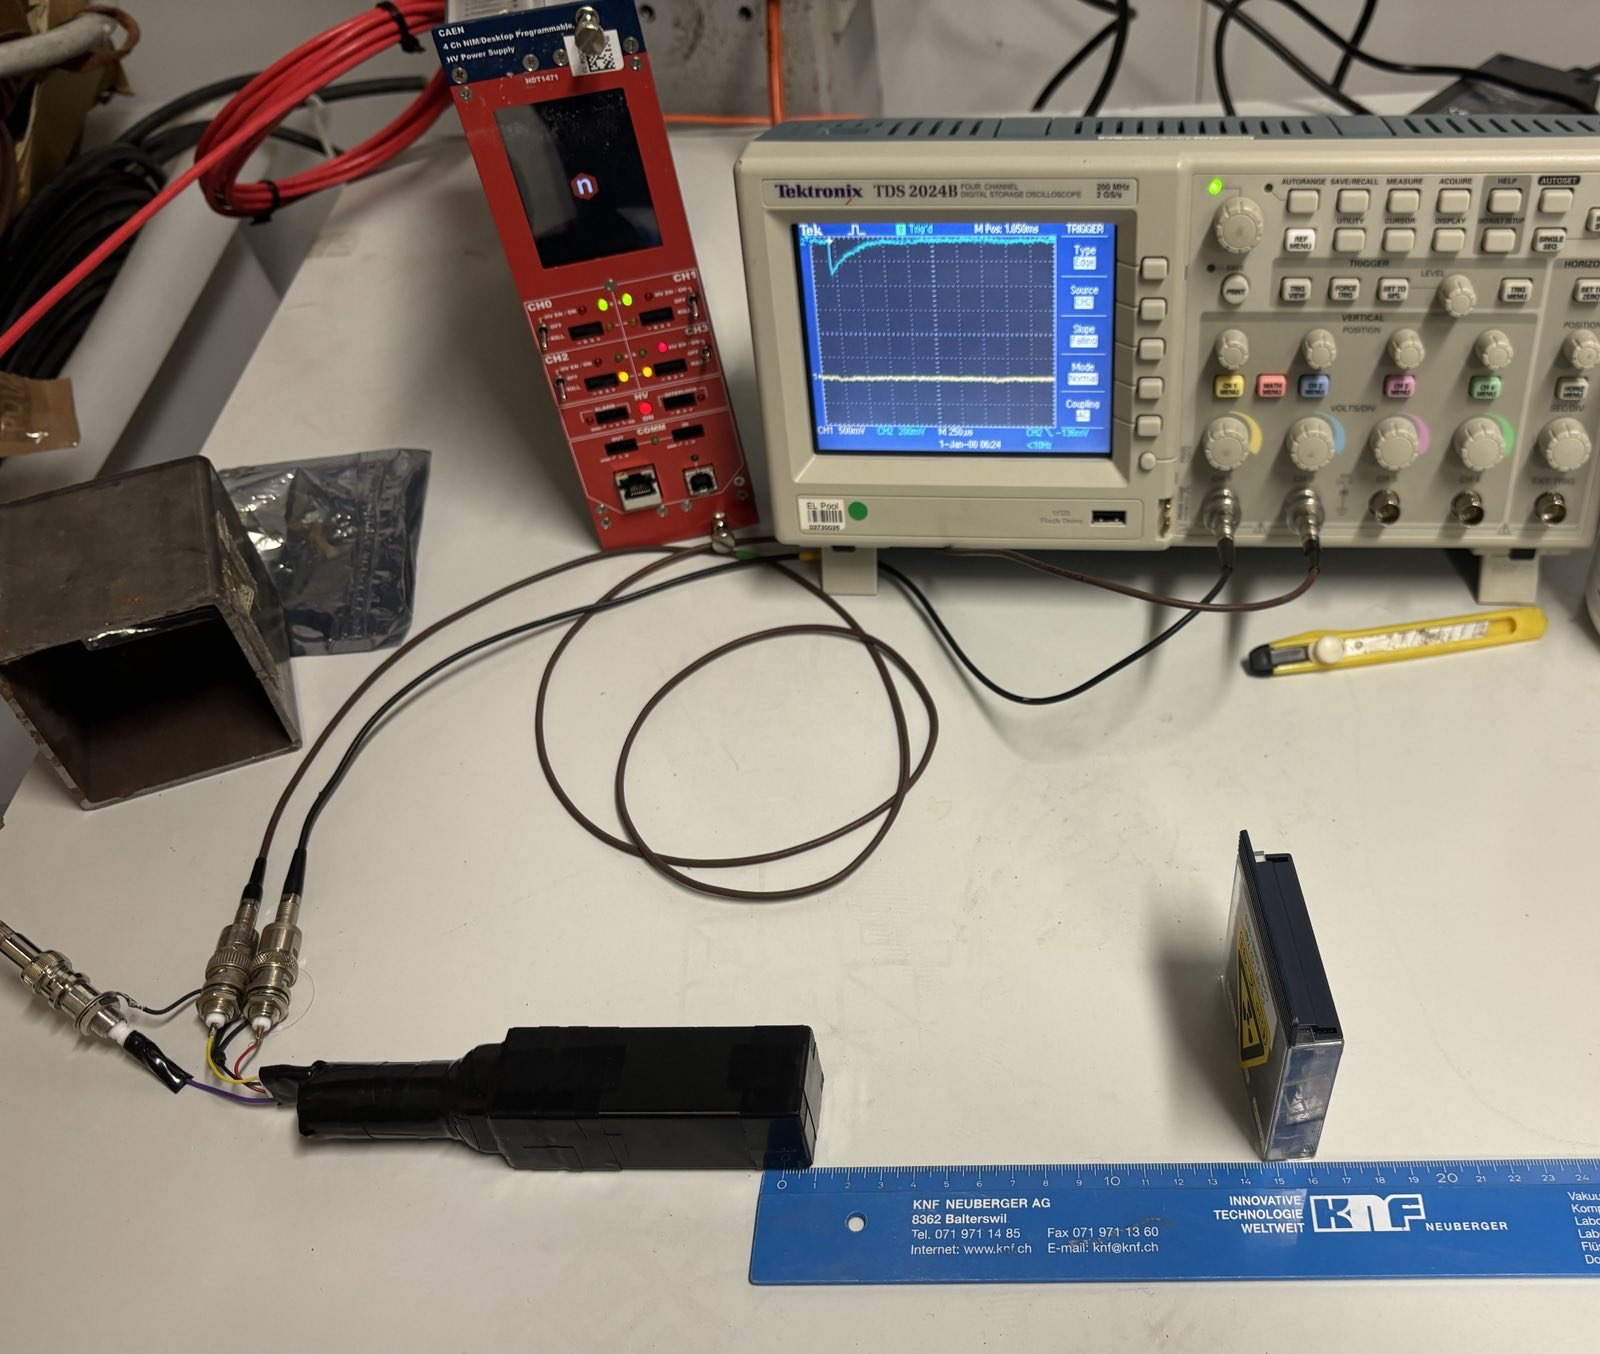
\includegraphics[width=0.7\textwidth, frame]{images/pmt_spectroscopy_setup.jpg}
            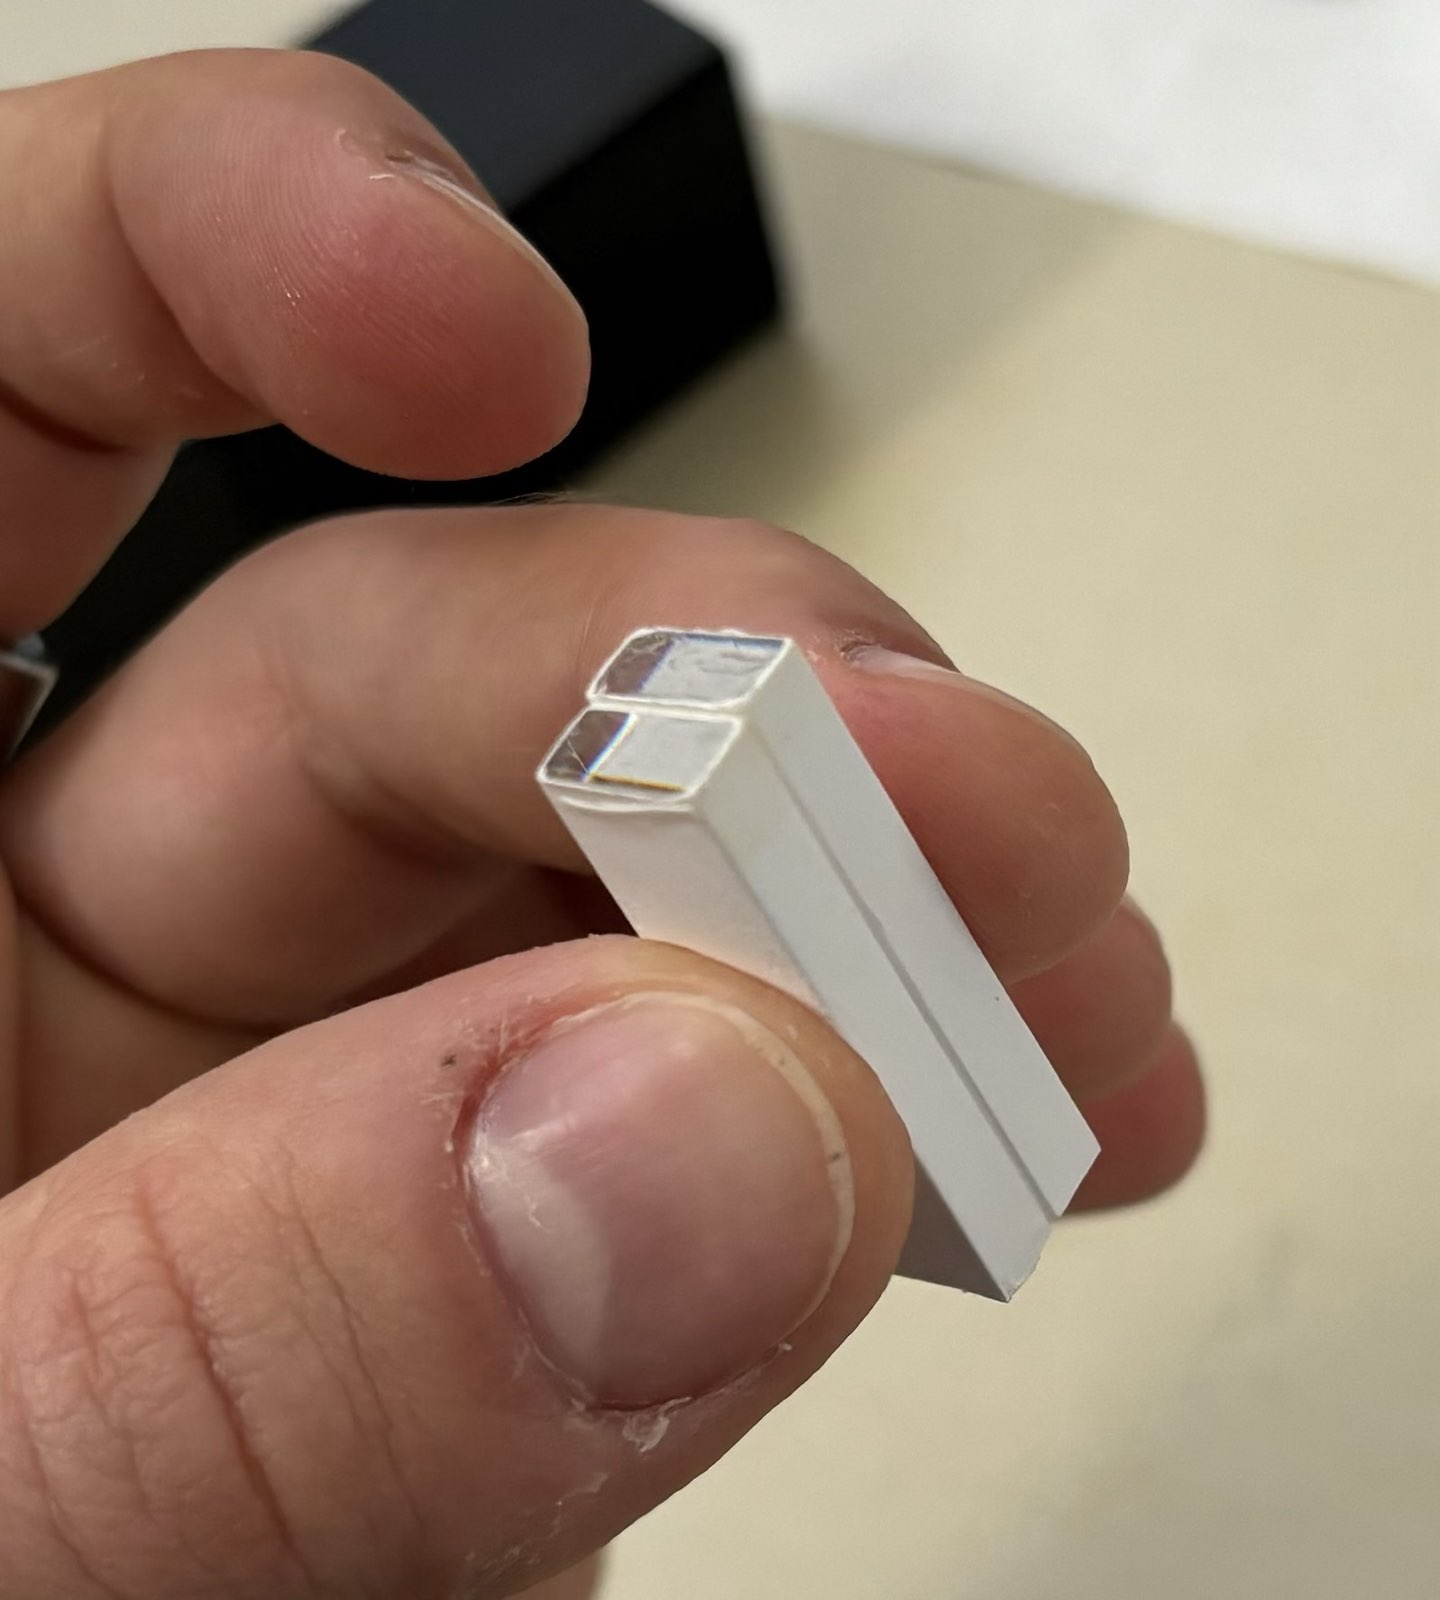
\includegraphics[width=0.3\textwidth, frame]{images/wrapped_crystals.jpg}
        \end{figure}
    \end{column}
    \begin{column}{0.5\textwidth}
        \begin{itemize}
            \item An enclosure was designed and 3D-printed to hold the PMT and two intact crystals
            \item The signal is read out via an osciloscope
        \end{itemize}
    \end{column}
\end{columnframe}

\begin{columnframe}{PMT Spectroscopy Raw Results}
    \begin{column}{0.5\textwidth}
        \begin{figure}
            \centering
            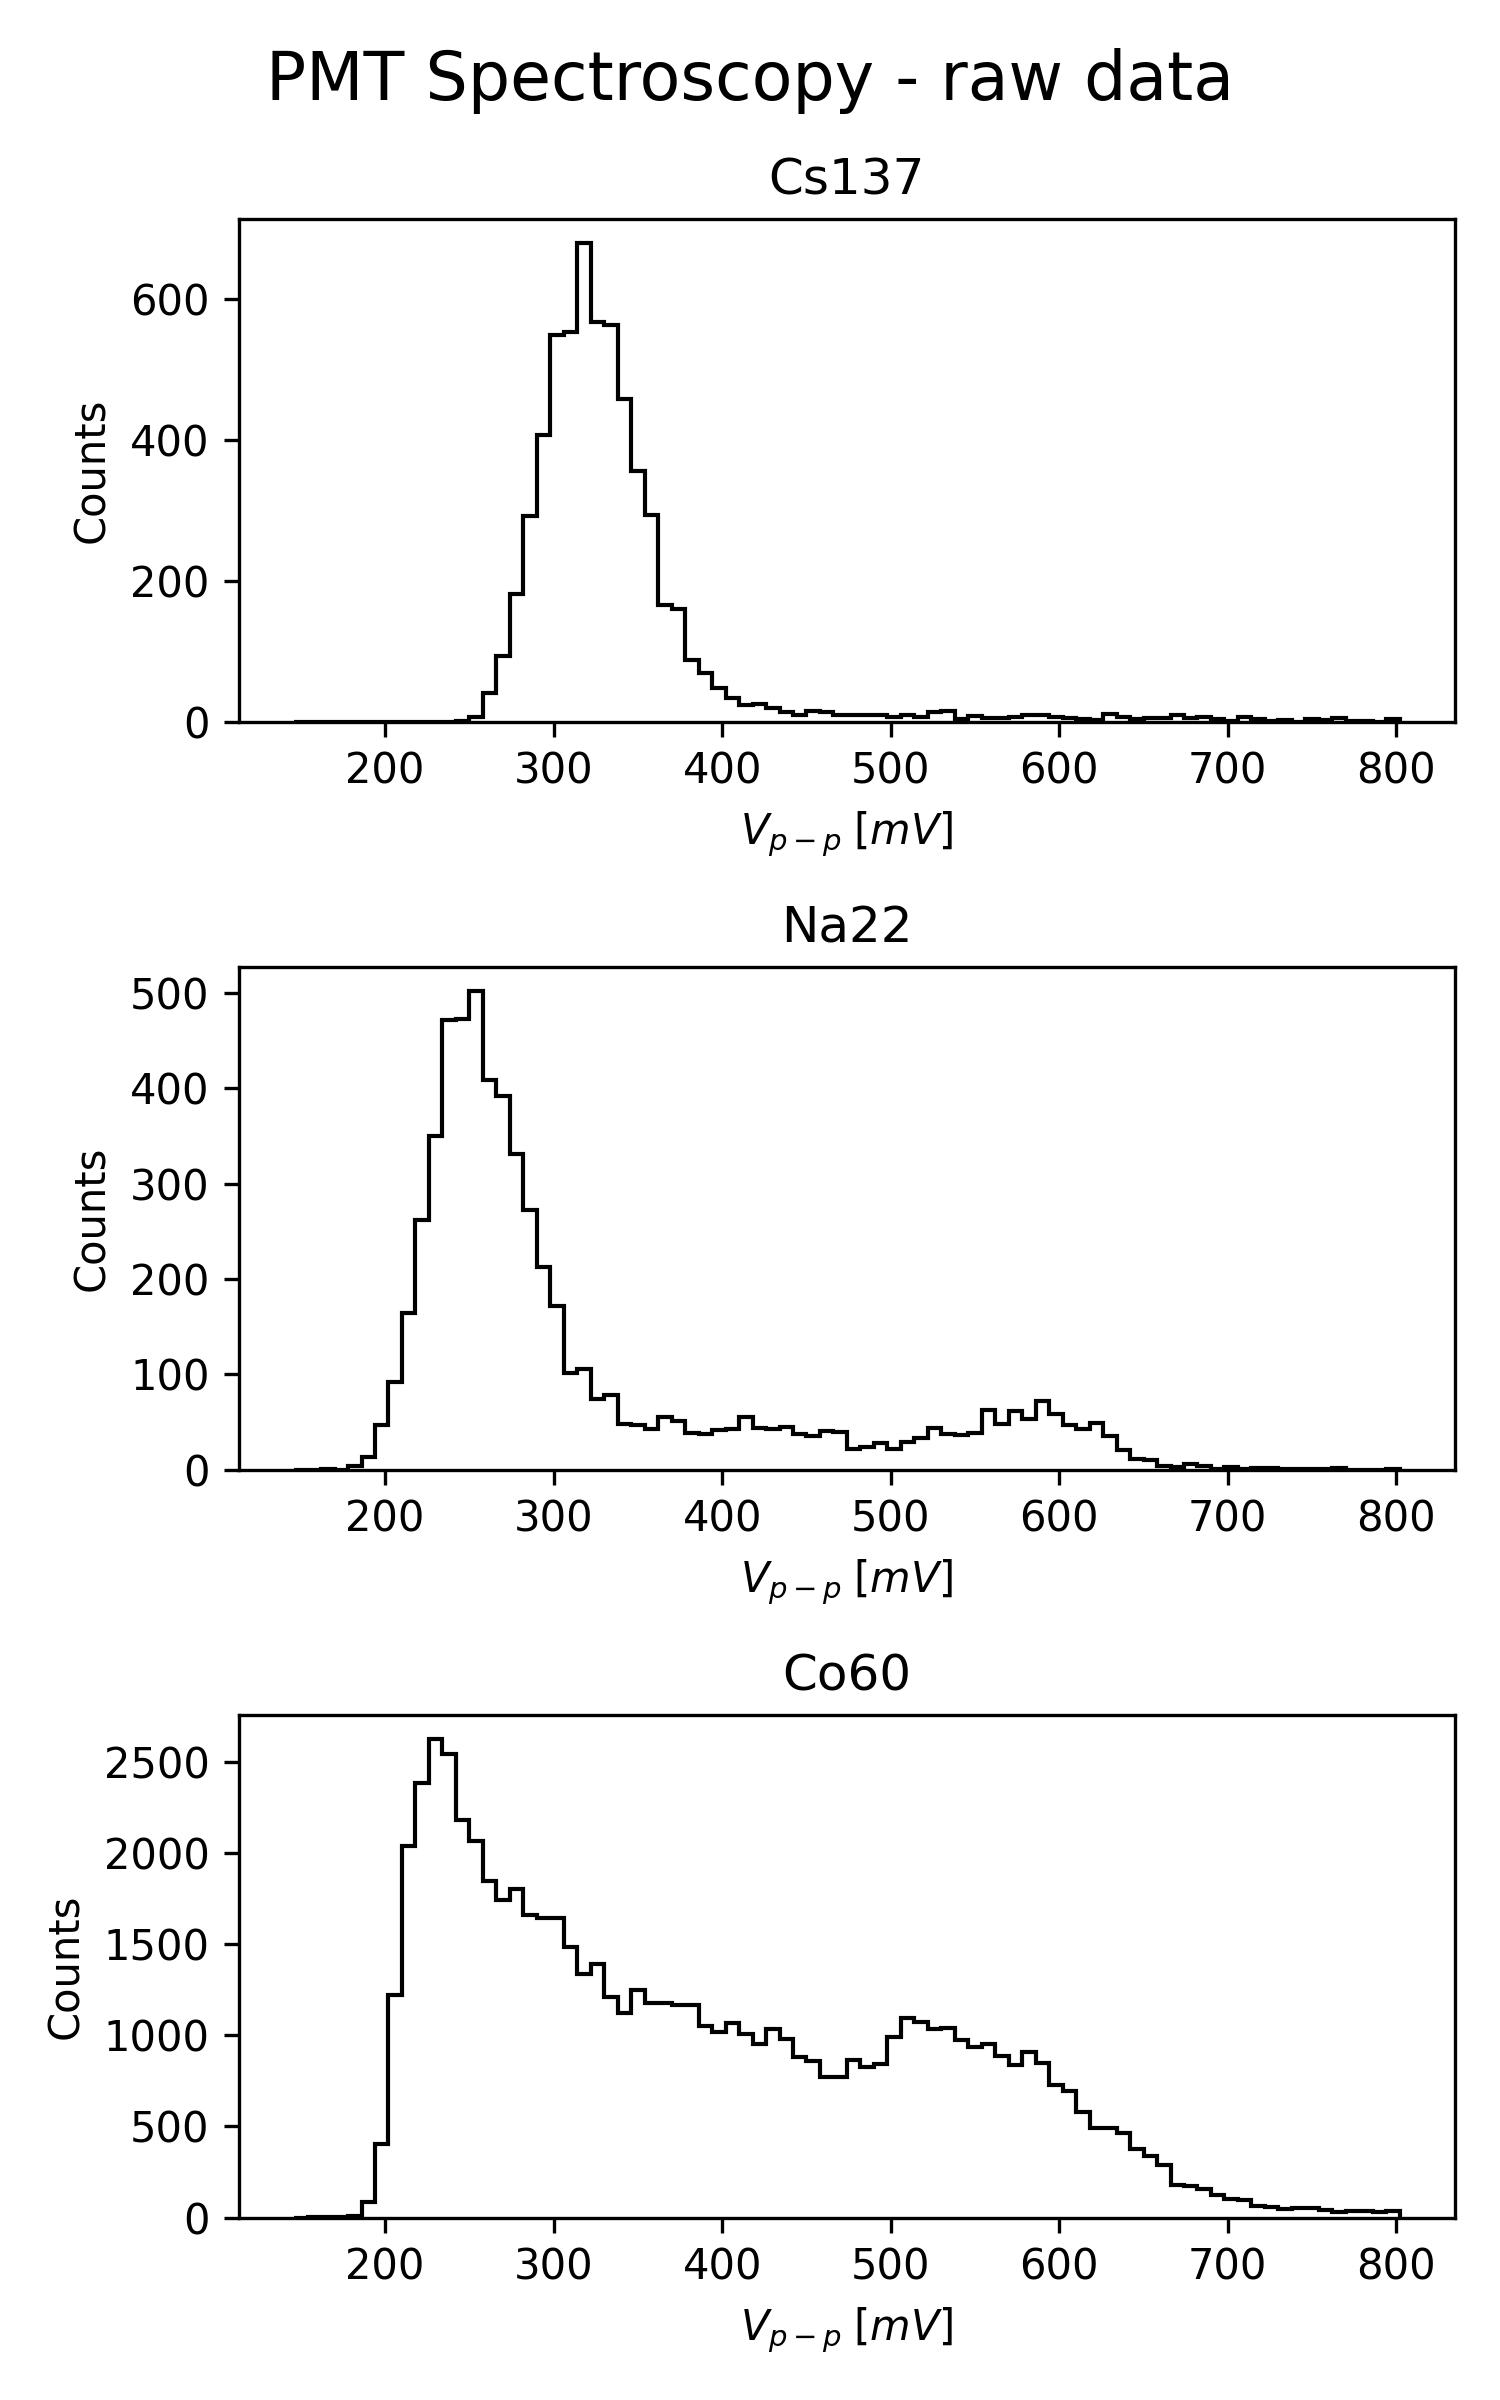
\includegraphics[width=0.65\textwidth]{images/pmt_raw_spectra.jpg}
        \end{figure}
    \end{column}
    \begin{column}{0.5\textwidth}
        \begin{itemize}
            \item Reminder: Co-60 peaks at 1.17 and 1.33 \MeV
            \item Reminder: Na-22 peaks at 511 \keV and 1275 \keV
            \item Reminder: Cs-137 peaks at 662 \keV
            \item The peaks are visible, but not very pronounced - therefore we proceed to fitting
        \end{itemize}
    \end{column}
\end{columnframe}

\begin{frame}[plain]
    \begin{columns}
        \begin{column}{0.5\textwidth}
            \begin{figure}
                \centering
                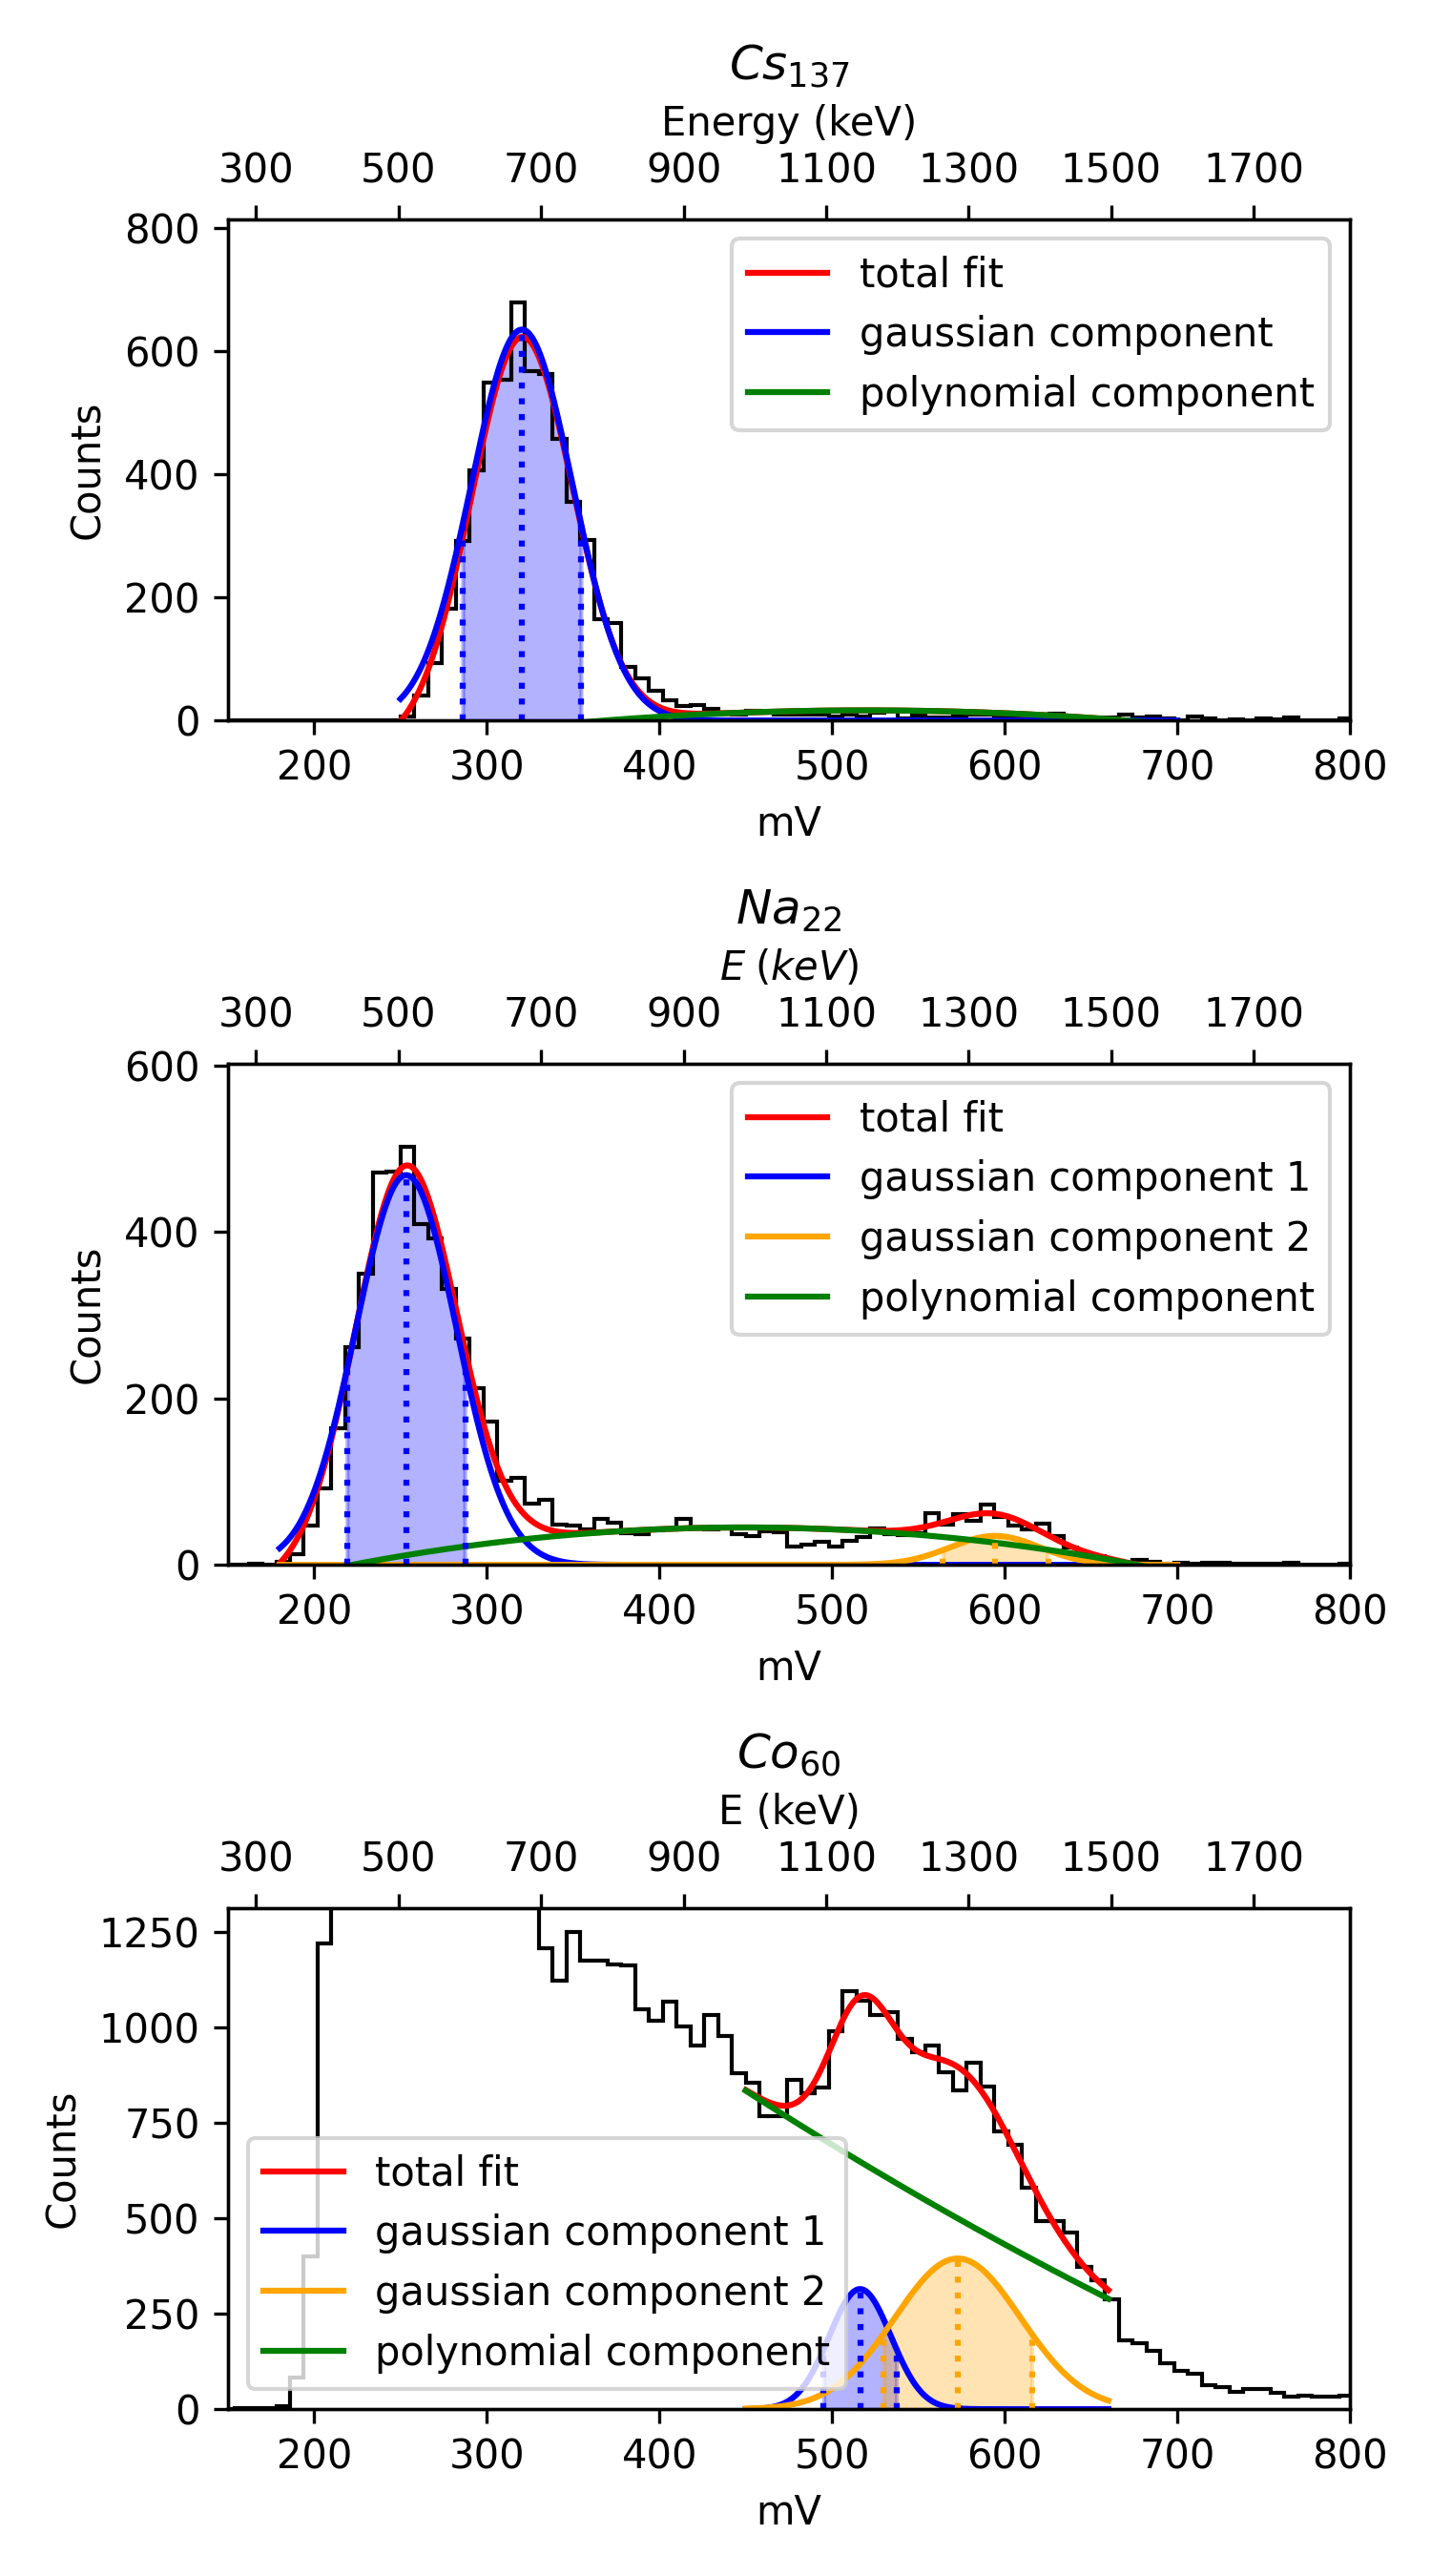
\includegraphics[width=0.85\textwidth]{images/pmt_spectra.png}
            \end{figure}
        \end{column}
        \begin{column}{0.5\textwidth}
            \begin{itemize}
                \item The peaks are fitted with gaussian functions
                \item Background is modelled with a polynomial or exponential function
                \item Calibration is done using the known energies of the peaks
                \item Reminder: Co-60 (1170 and 1330 \keV), Na-22 (511 \keV and 1275 \keV), Cs-137 (662 \keV)
            \end{itemize}
        \end{column}
    \end{columns}
\end{frame}

\begin{columnframe}{SiPM Spectroscopy Setup}
    \begin{column}{0.5\textwidth}
        \begin{figure}
            \centering
            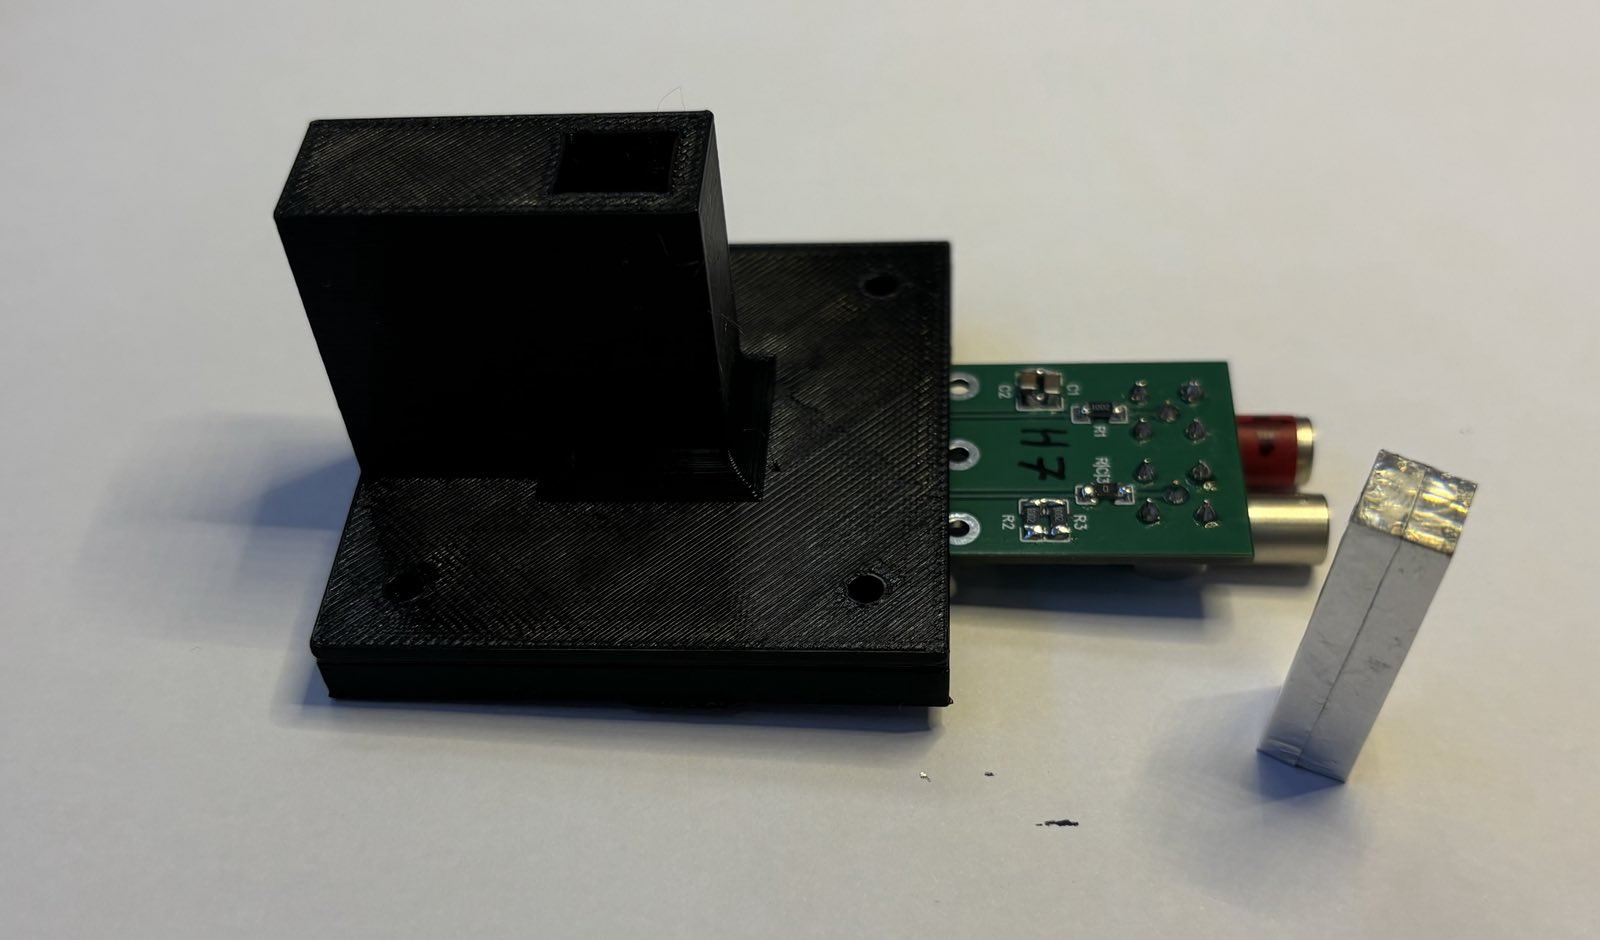
\includegraphics[trim=0 0 0 0, clip, width=0.8\textwidth, frame]{images/pcb_in_enclosure.jpg}
            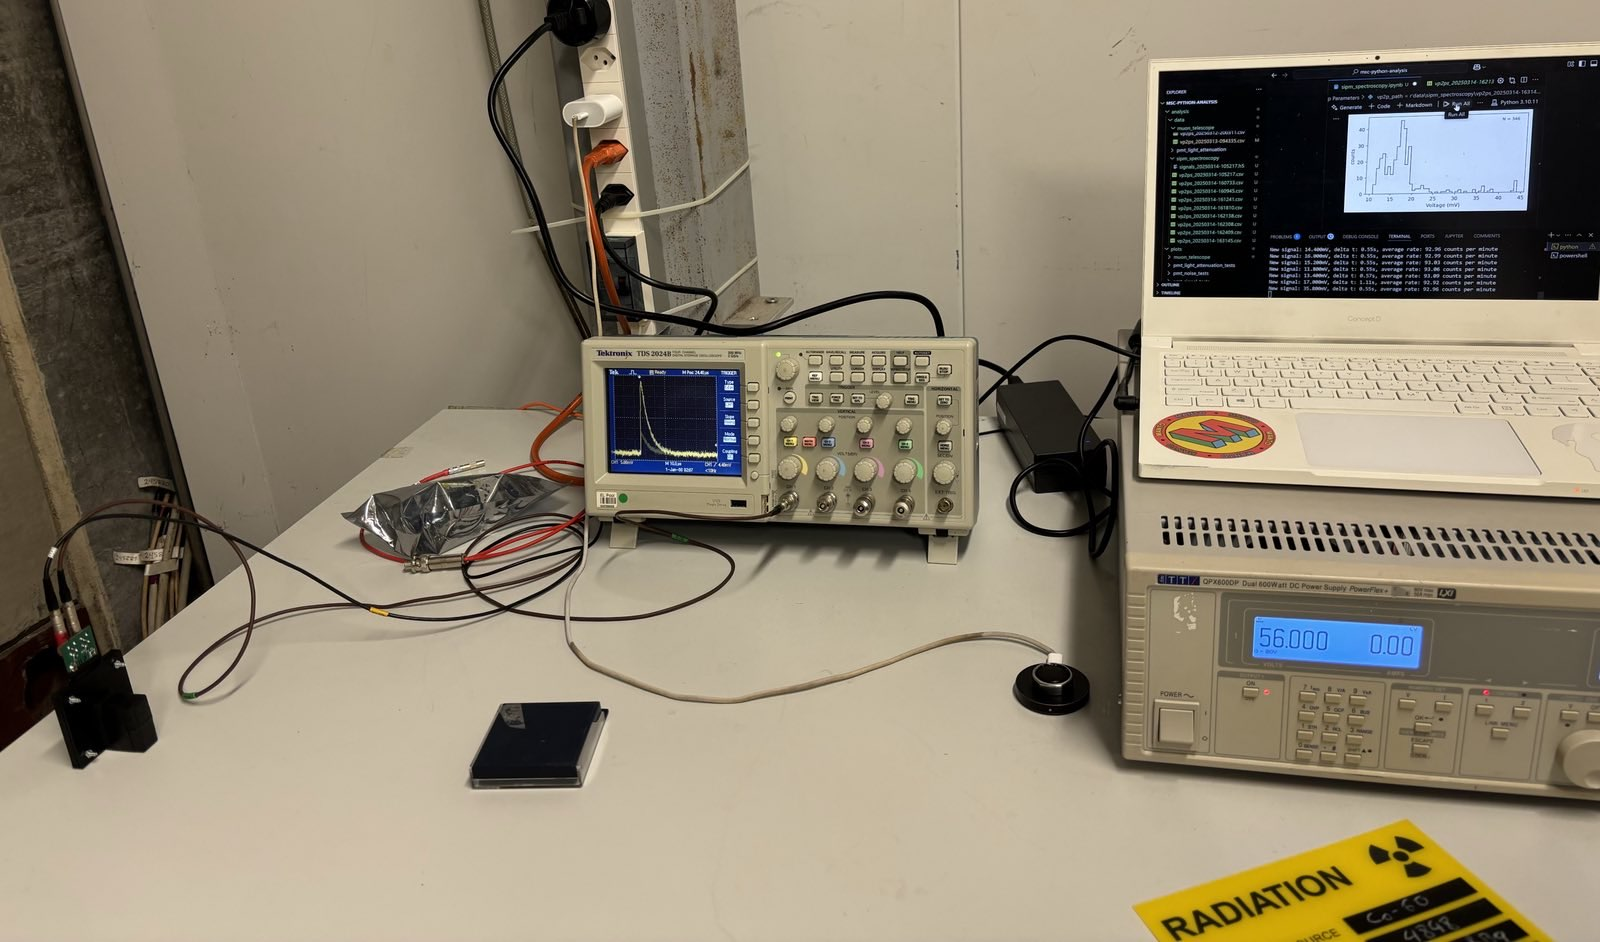
\includegraphics[trim=0 0 0 0, clip, width=0.8\textwidth, frame]{images/sipm_spectroscopy_setup.jpg}
        \end{figure}
    \end{column}
    \begin{column}{0.5\textwidth}
        \begin{itemize}
            \item An enclosure was designed and 3D-printed to hold the SiPM and two intact crystals
            \item The signal is once again read out via an osciloscope
        \end{itemize}
    \end{column}
\end{columnframe}

\begin{frame}[plain]
    \begin{columns}
        \begin{column}{0.5\textwidth}
            \begin{figure}
                \centering
                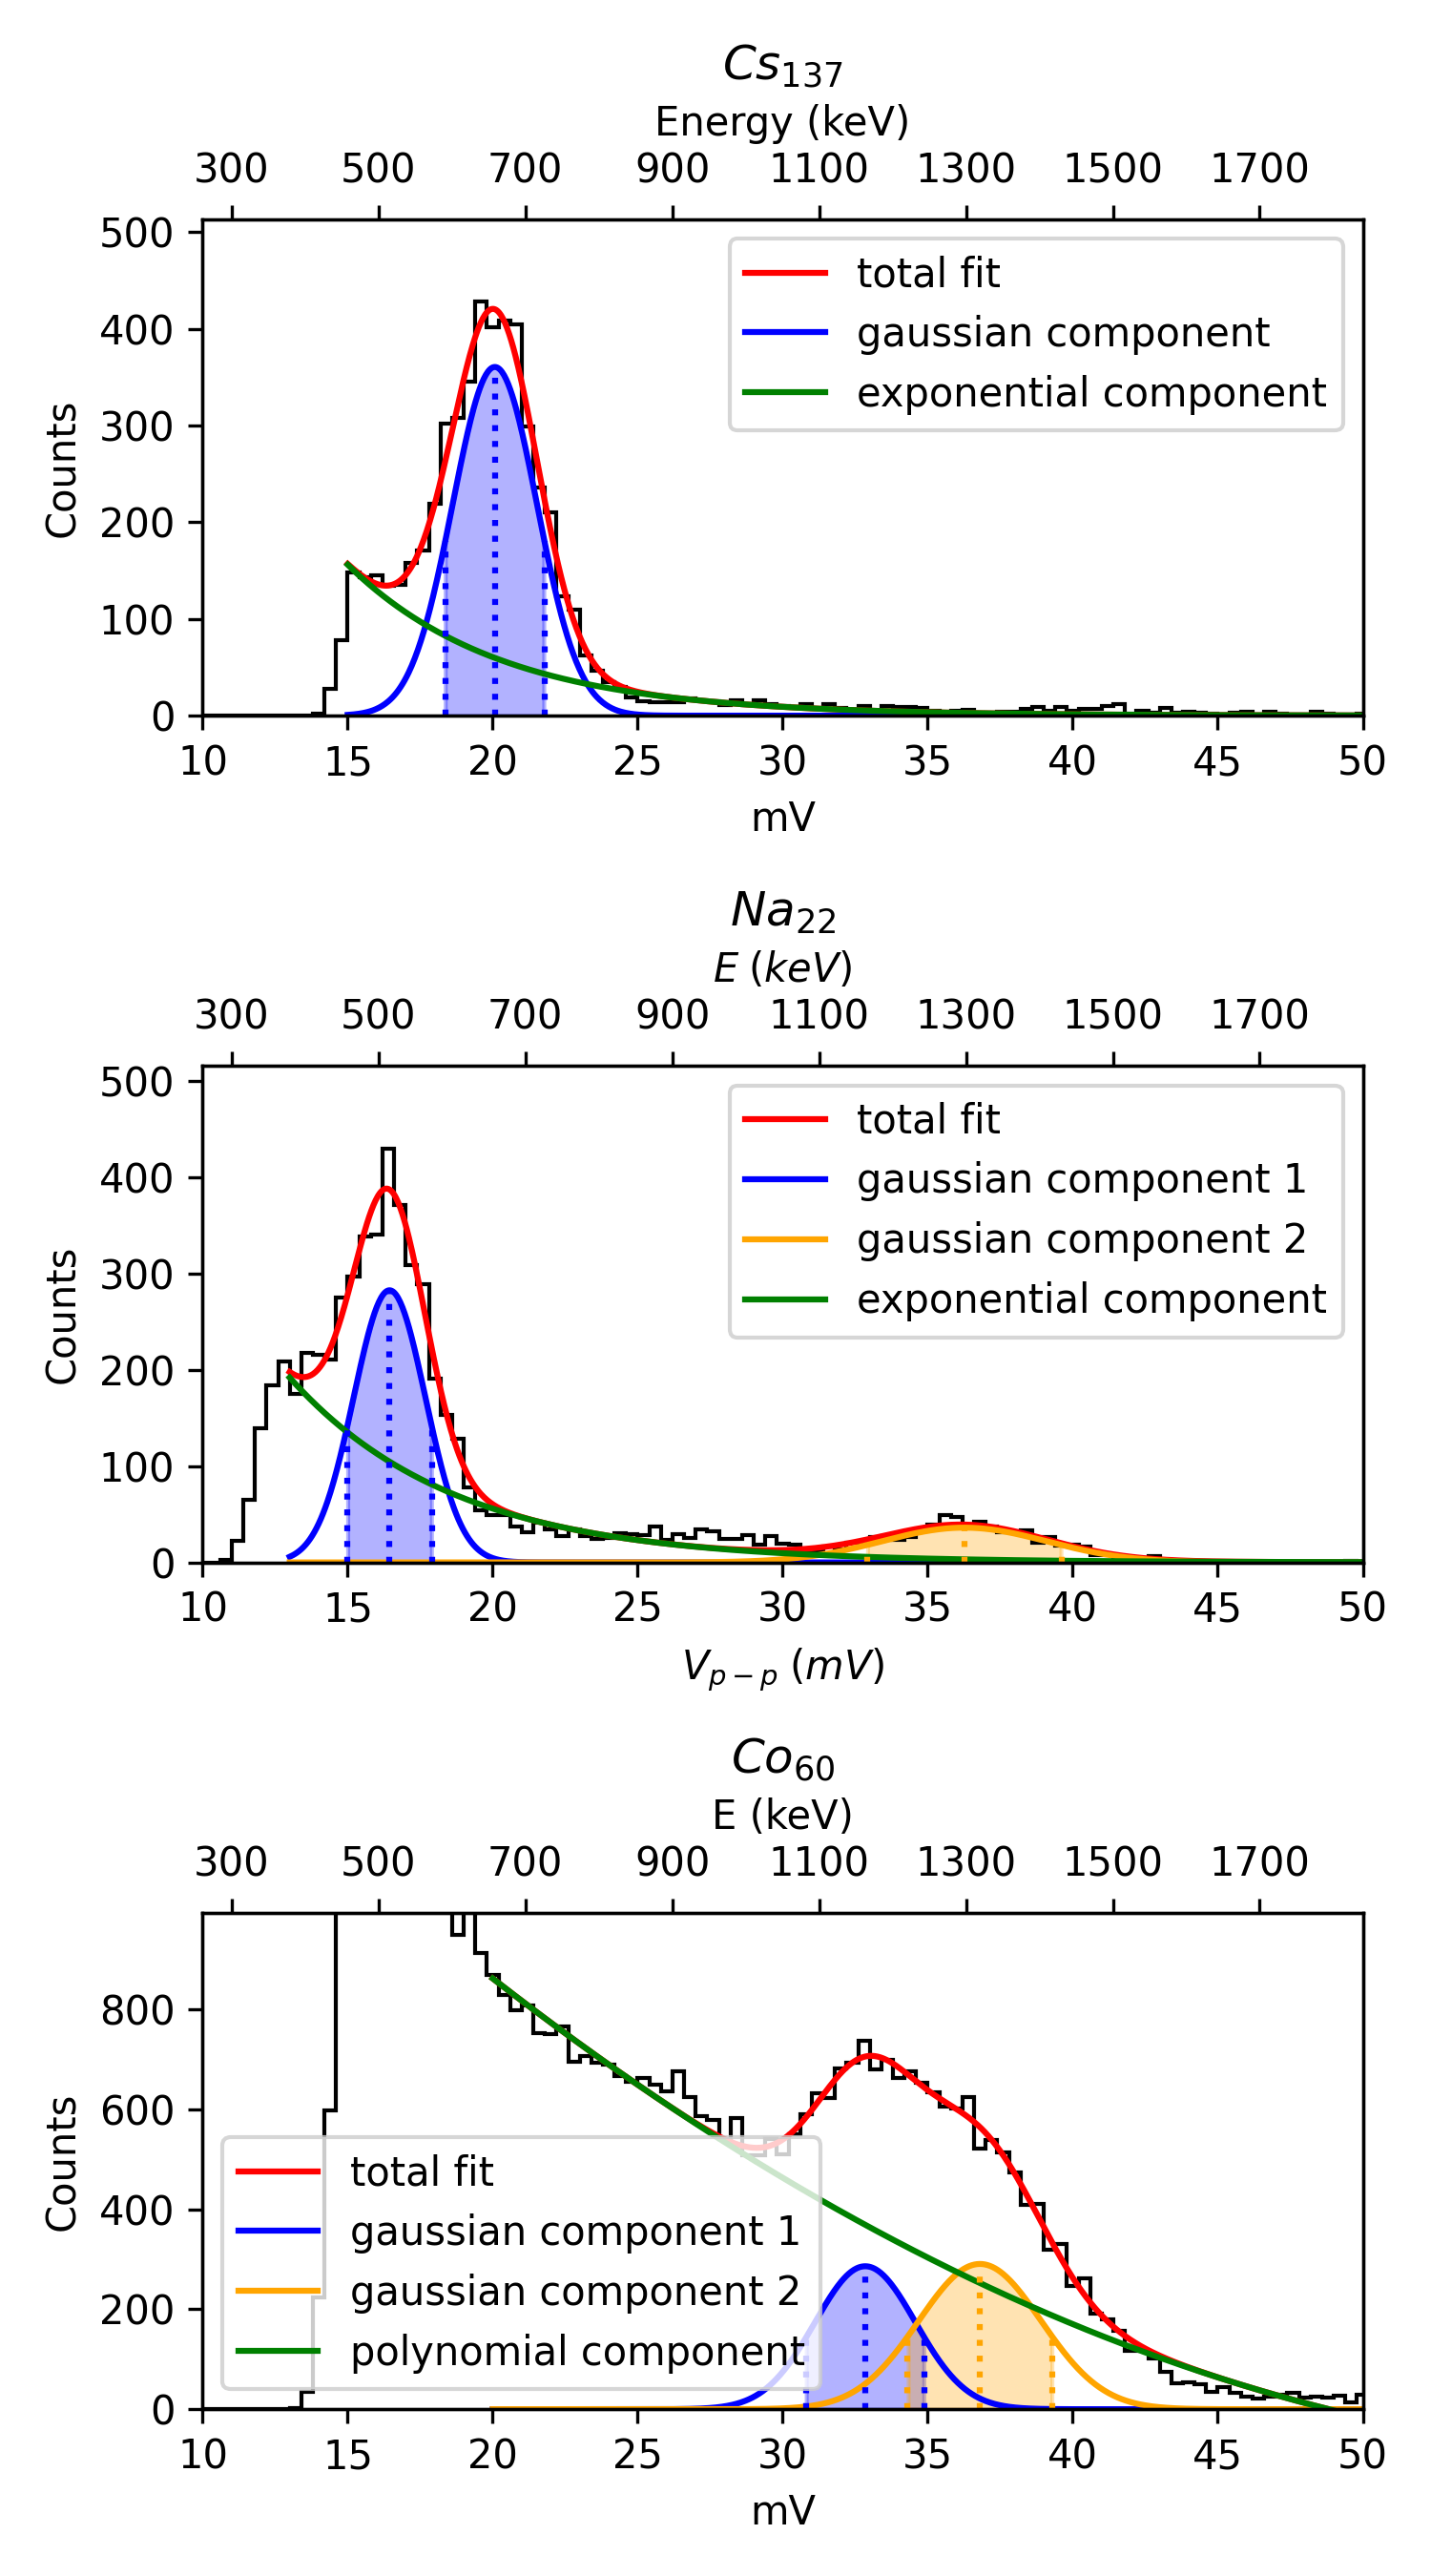
\includegraphics[width=0.85\textwidth]{images/sipm_spectra.png}
            \end{figure}
        \end{column}
        \begin{column}{0.5\textwidth}
            \begin{itemize}
                \item The peaks are fitted with gaussian functions
                \item Background is modelled with a polynomial function
                \item Calibration is done using the known energies of the peaks
                \item Reminder: Co-60 (1170 and 1330 \keV), Na-22 (511 \keV and 1275 \keV), Cs-137 (662 \keV)
            \end{itemize}
        \end{column}
    \end{columns}
\end{frame}

\begin{frame}{SiPM - PMT Energy Resolution Comparison}
    \begin{columns}
        \begin{column}{0.5\textwidth}
            \begin{figure}
                \centering
                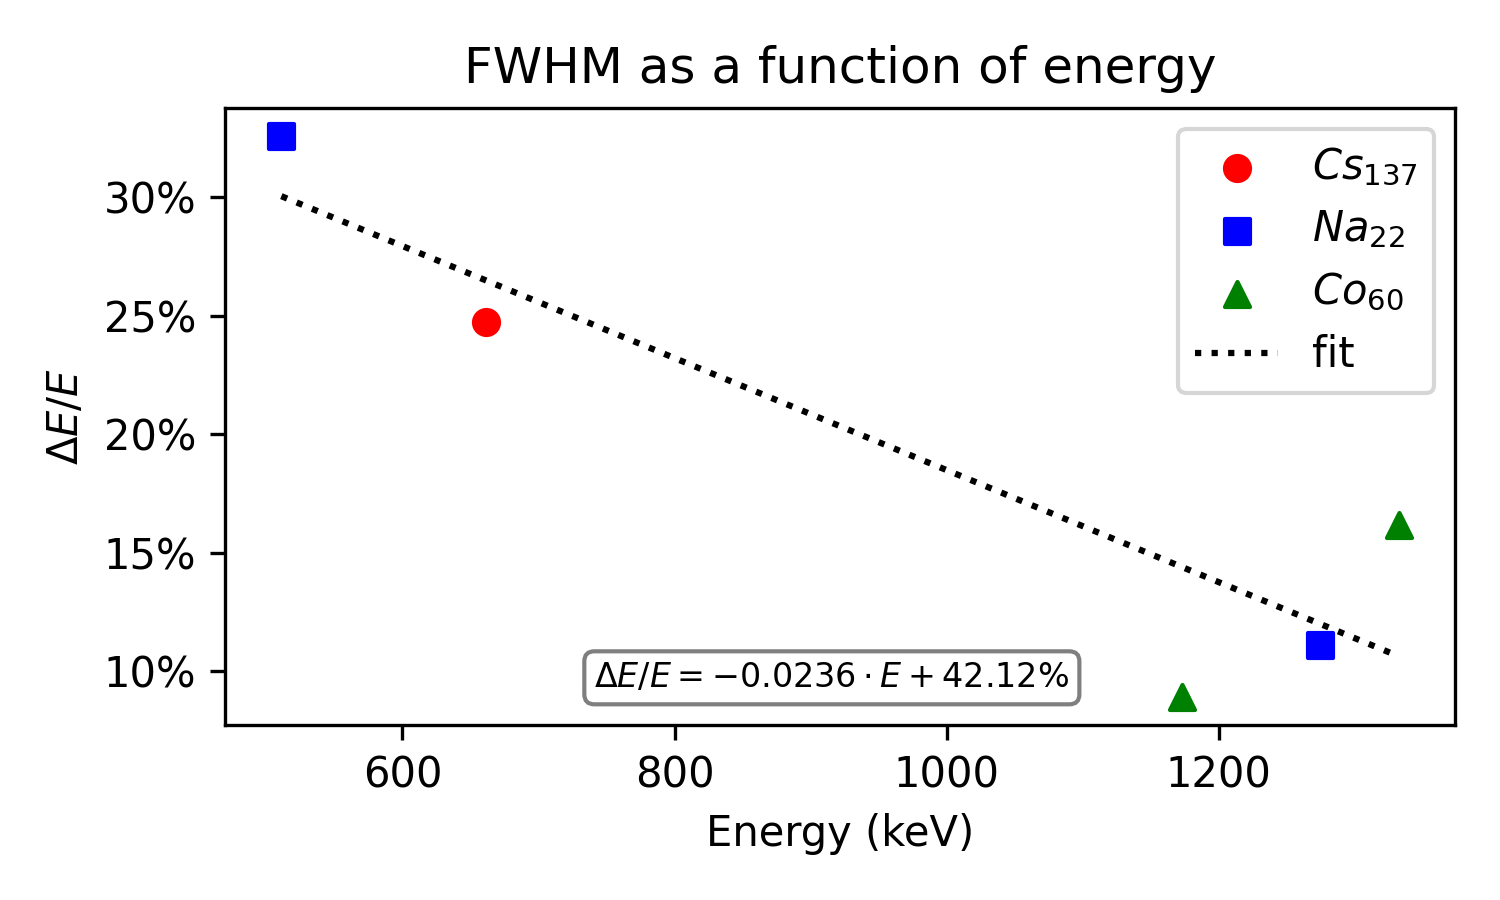
\includegraphics[width=0.8\textwidth]{images/PMT_dE_ov_E.png}
                \caption{PMT energy resolution as a function of energy}
            \end{figure}
        \end{column}
        \begin{column}{0.5\textwidth}
            \begin{figure}
                \centering
                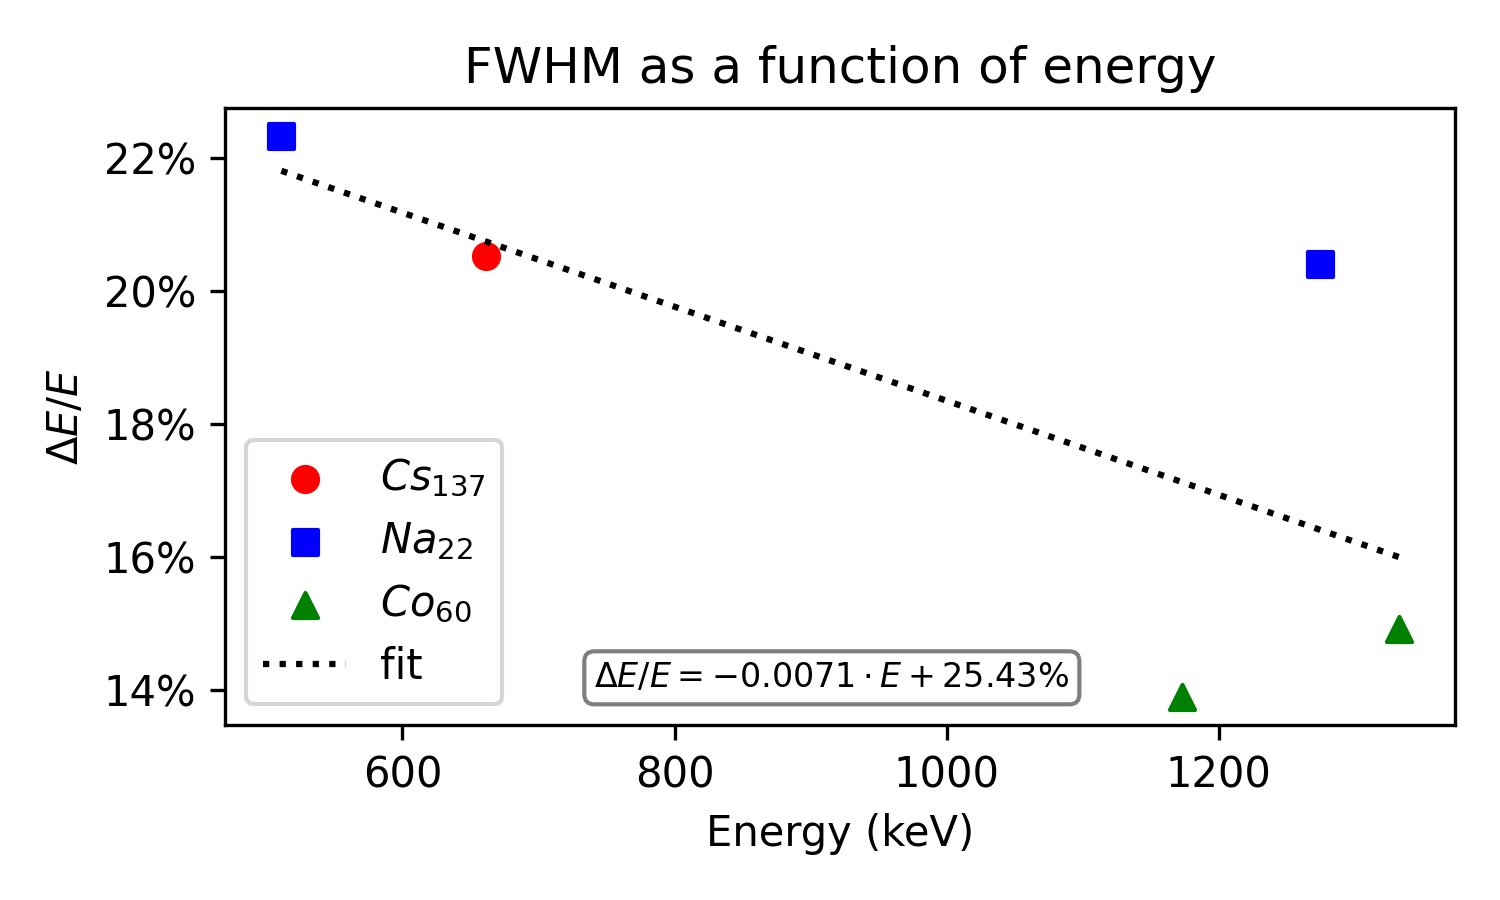
\includegraphics[width=0.8\textwidth]{images/SiPM_dE_ov_E.png}
                \caption{SiPM energy resolution as a function of energy}
            \end{figure}
        \end{column}
    \end{columns}
\end{frame}

\begin{frame}[plain]
    \begin{columns}
        \begin{column}{0.5\textwidth}
            \begin{figure}
                \centering
                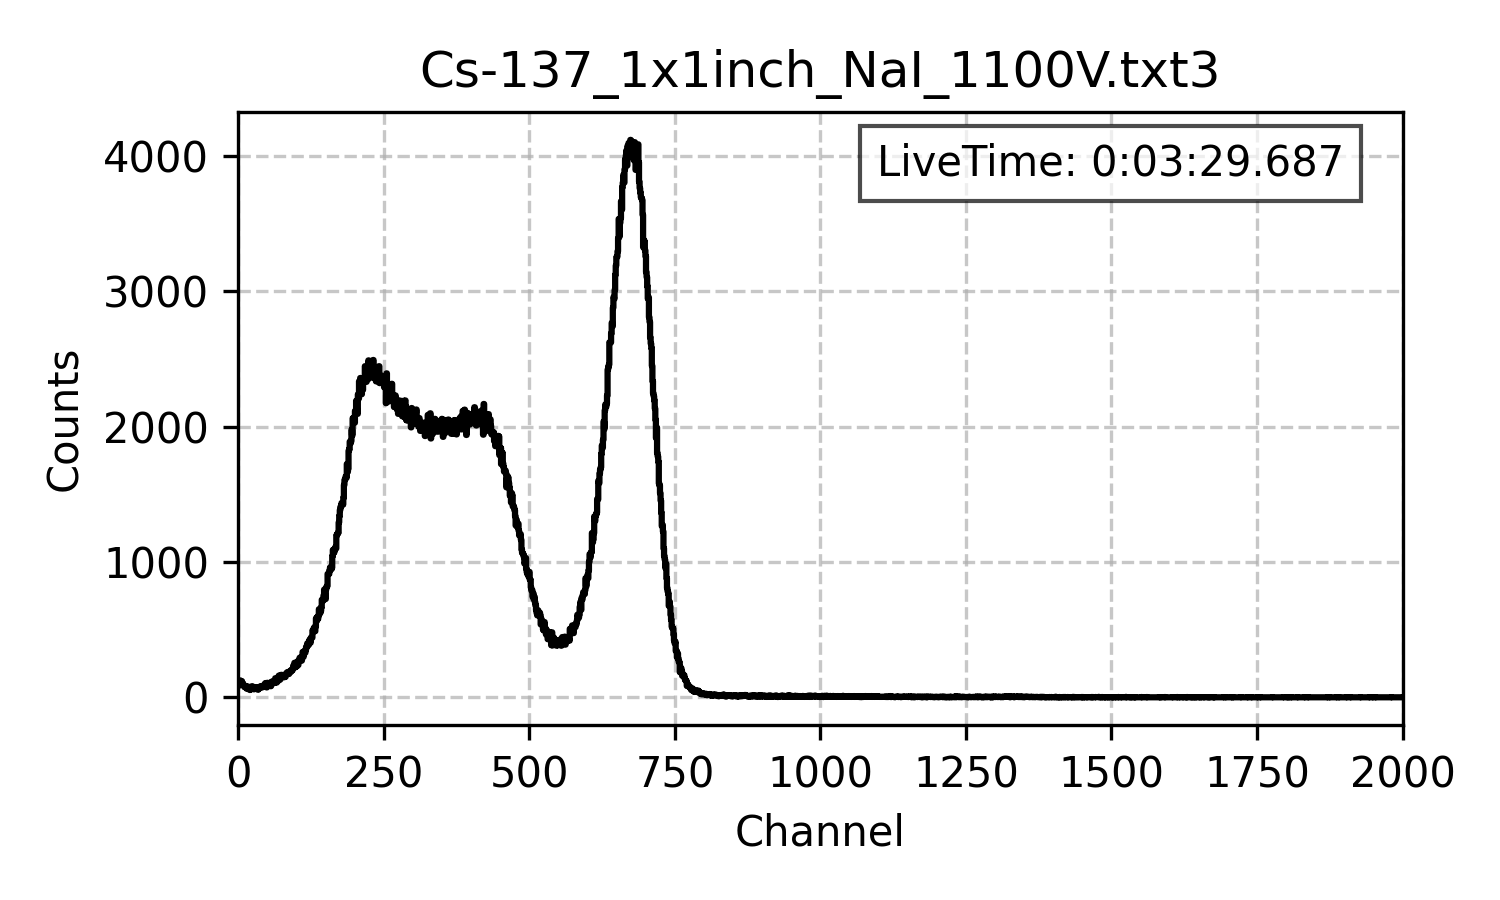
\includegraphics[width=0.85\textwidth]{images/Cs-137_1x1inch_NaI_1100V.png}
                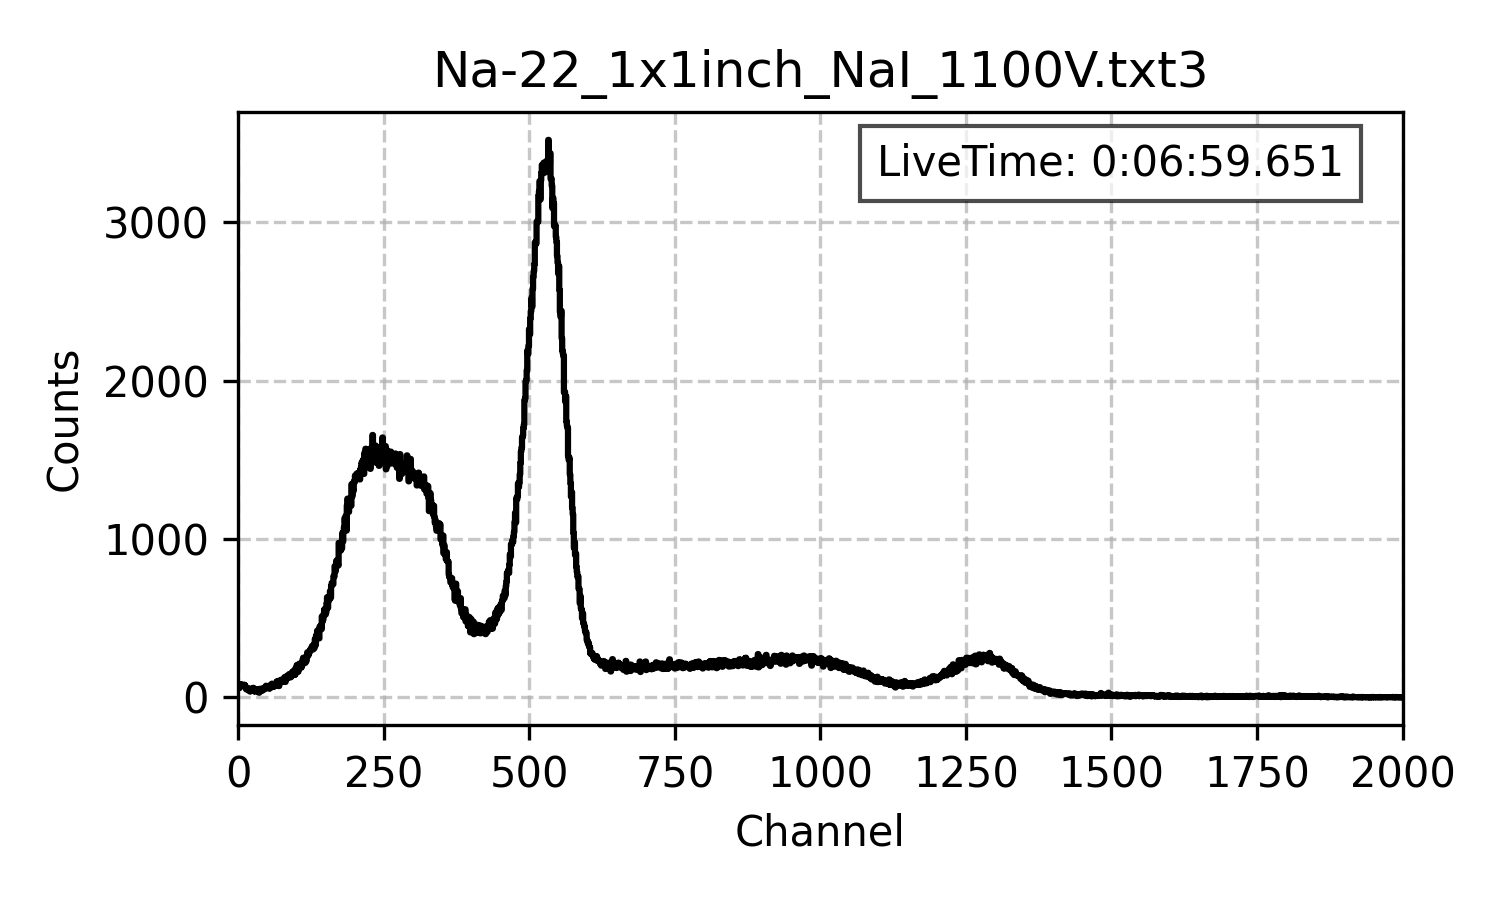
\includegraphics[width=0.85\textwidth]{images/Na-22_1x1inch_NaI_1100V.png}
                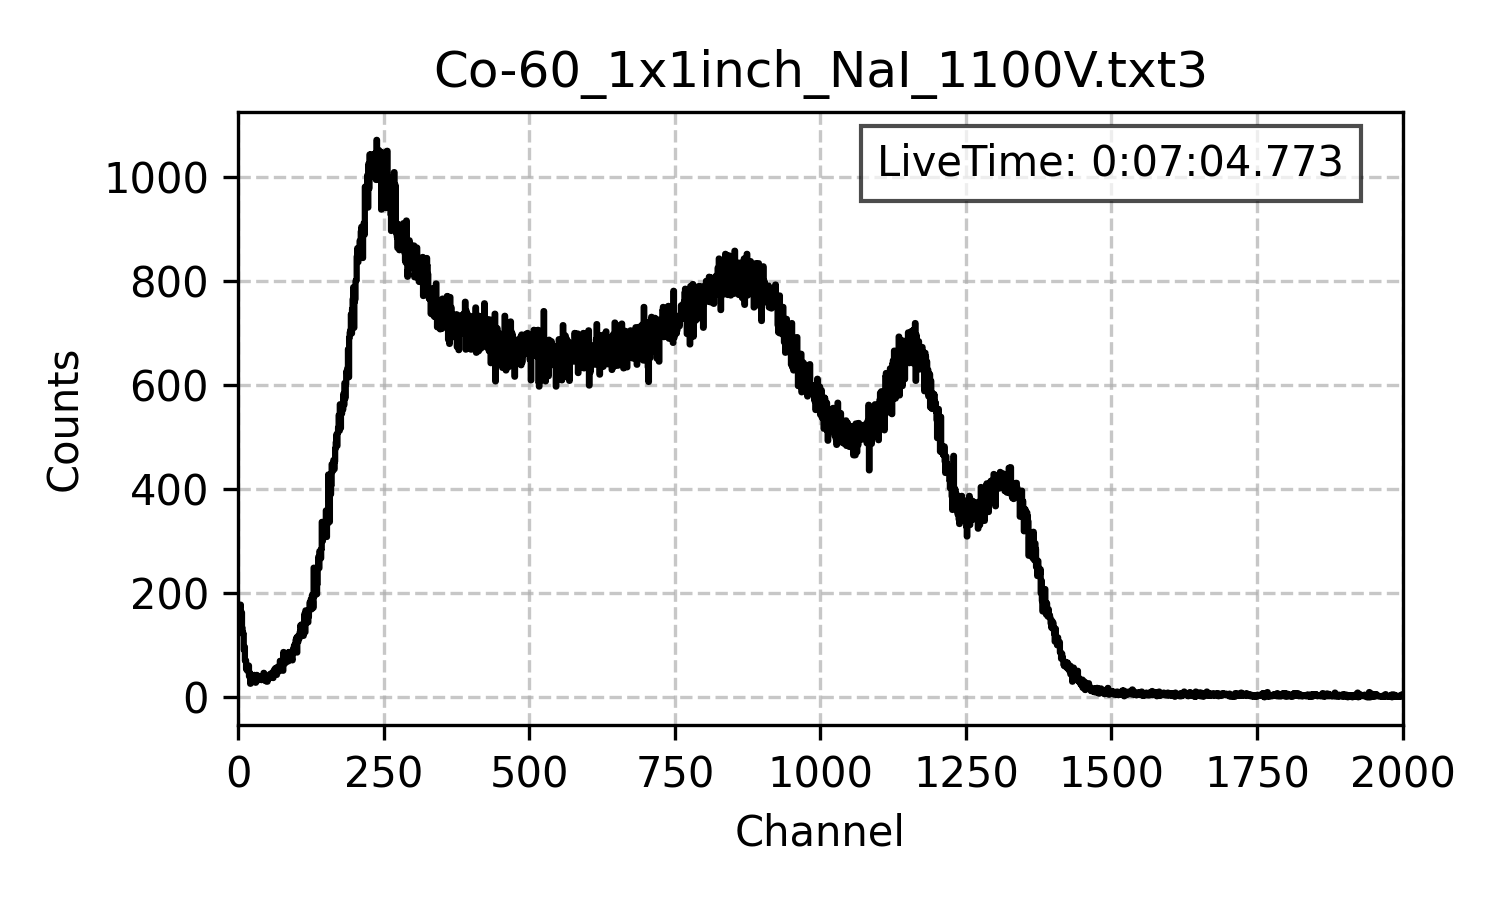
\includegraphics[width=0.85\textwidth]{images/Co-60_1x1inch_NaI_1100V.png}

            \end{figure}
        \end{column}
        \begin{column}{0.5\textwidth}
            \begin{itemize}
                \item Recent developments have revealed that the detector can benefit from a change of scintillator
                \item Results from an NaI crystal with a working voltage of 1100 \si{\volt} are shown
                \item The energy resolution is significantly better than that of the BGO-PMT
                \item Reminder: Cs-137 (662 \keV), Na-22 (511 \keV and 1275 \keV), Co-60 (1170 and 1330 \keV)
            \end{itemize}

            \vspace{0.5cm}
            \imagesource{Courtesy of Mgr. Łukasz Adamowski (NCBJ)}
        \end{column}
    \end{columns}
\end{frame}

\begin{frame}[plain]
    \begin{columns}
        \begin{column}{0.5\textwidth}
            \begin{figure}
                \centering
                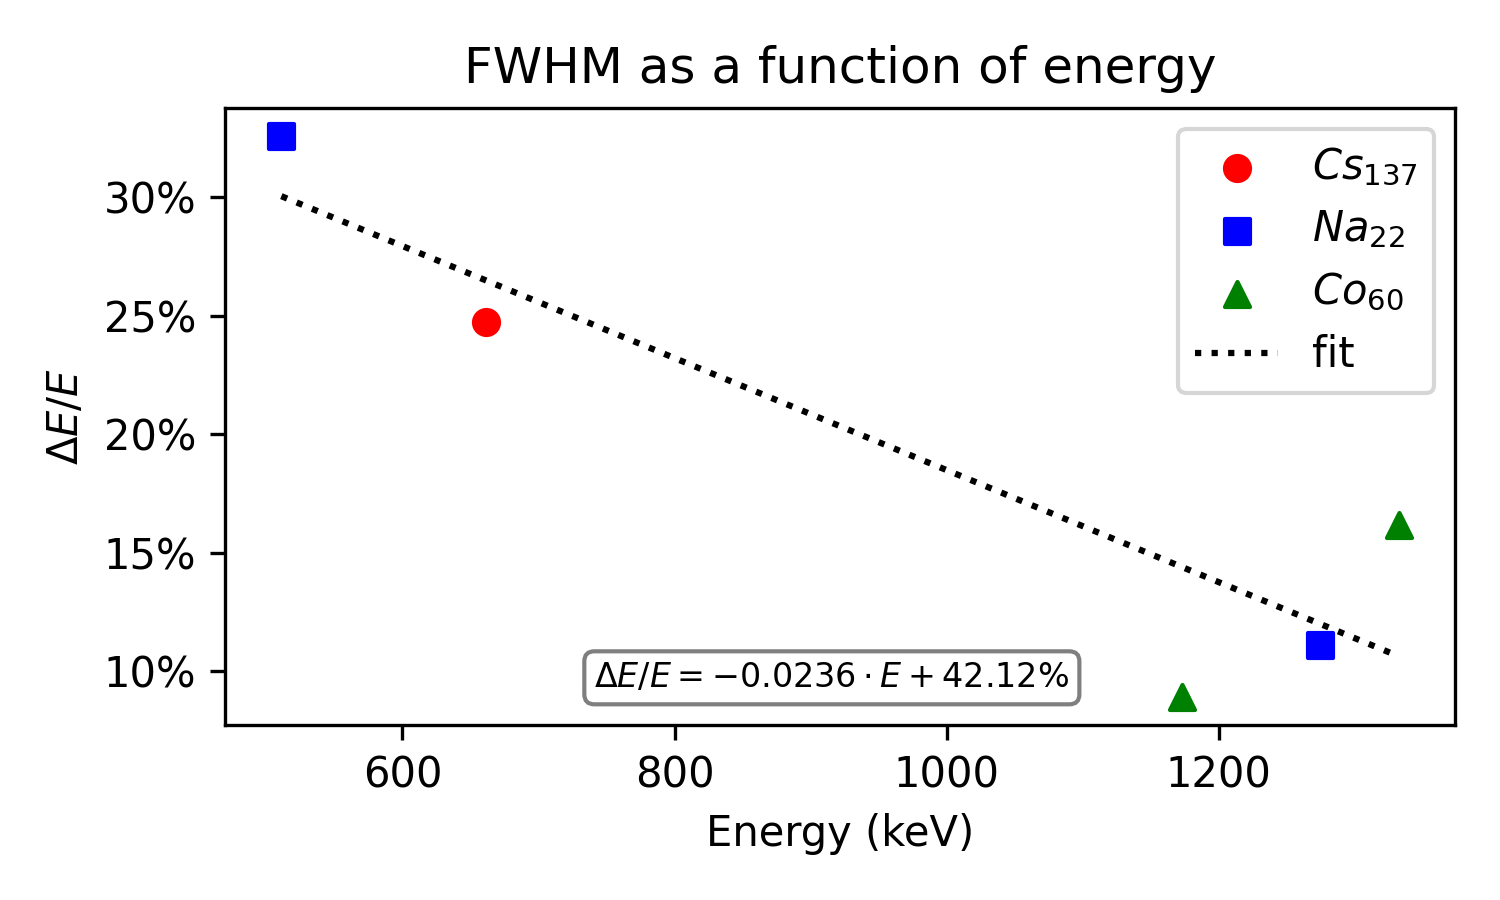
\includegraphics[width=0.8\textwidth]{images/PMT_dE_ov_E.png}
                \caption{PMT energy resolution as a function of energy}
            \end{figure}
        \end{column}
        \begin{column}{0.5\textwidth}
            \begin{figure}
                \centering
                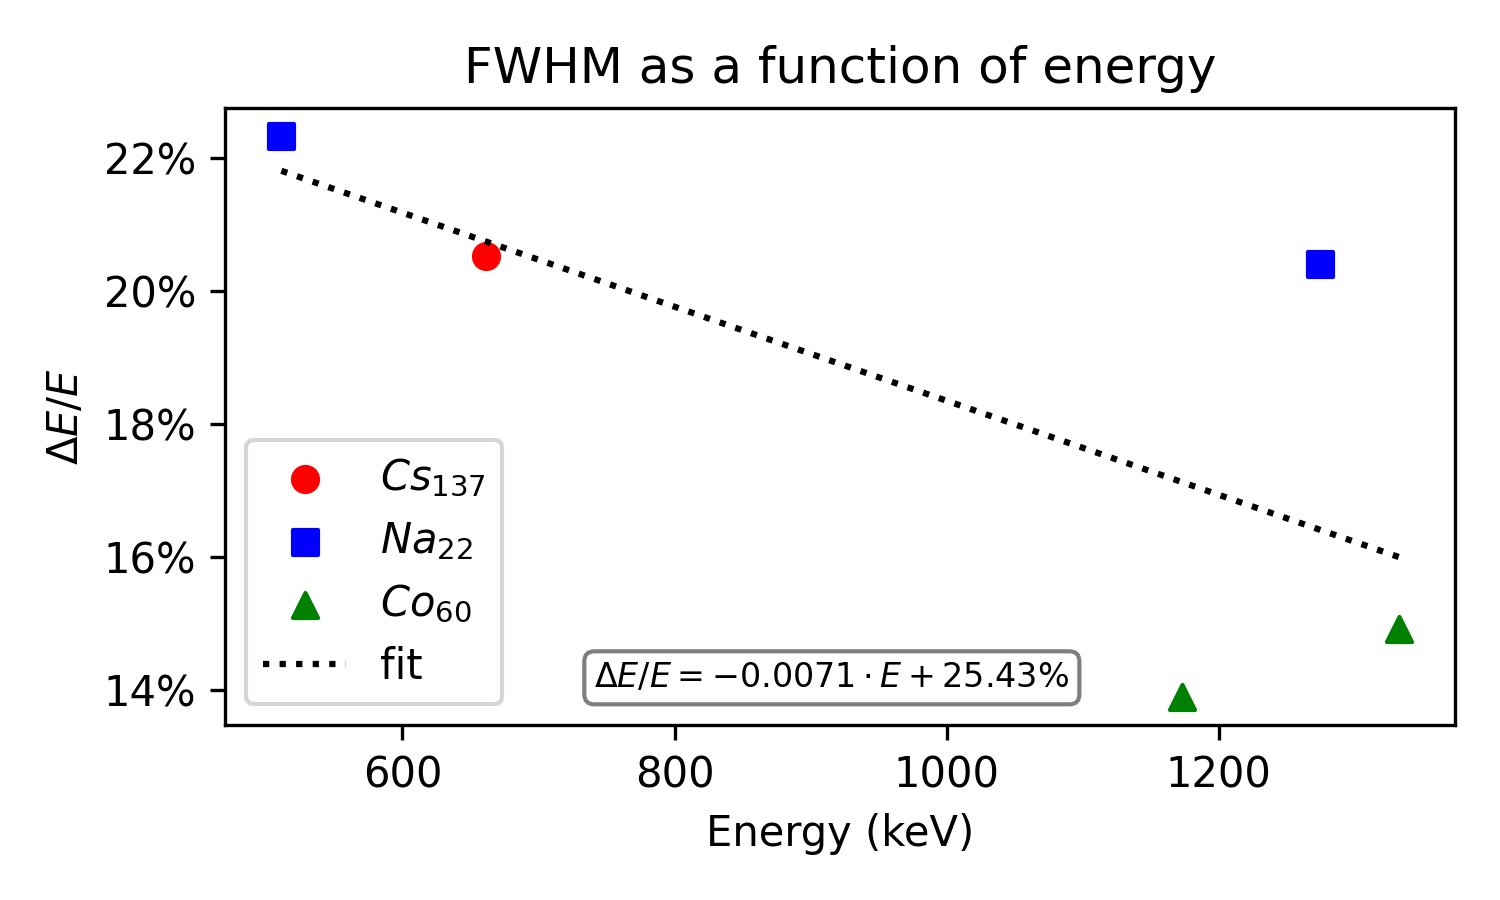
\includegraphics[width=0.8\textwidth]{images/SiPM_dE_ov_E.png}
                \caption{SiPM energy resolution as a function of energy}
            \end{figure}
        \end{column}
    \end{columns}
\end{frame}

\begin{columnframe}{Lastly... a Muon Telescope}
    \begin{column}{0.5\textwidth}
        \begin{figure}
            \centering
            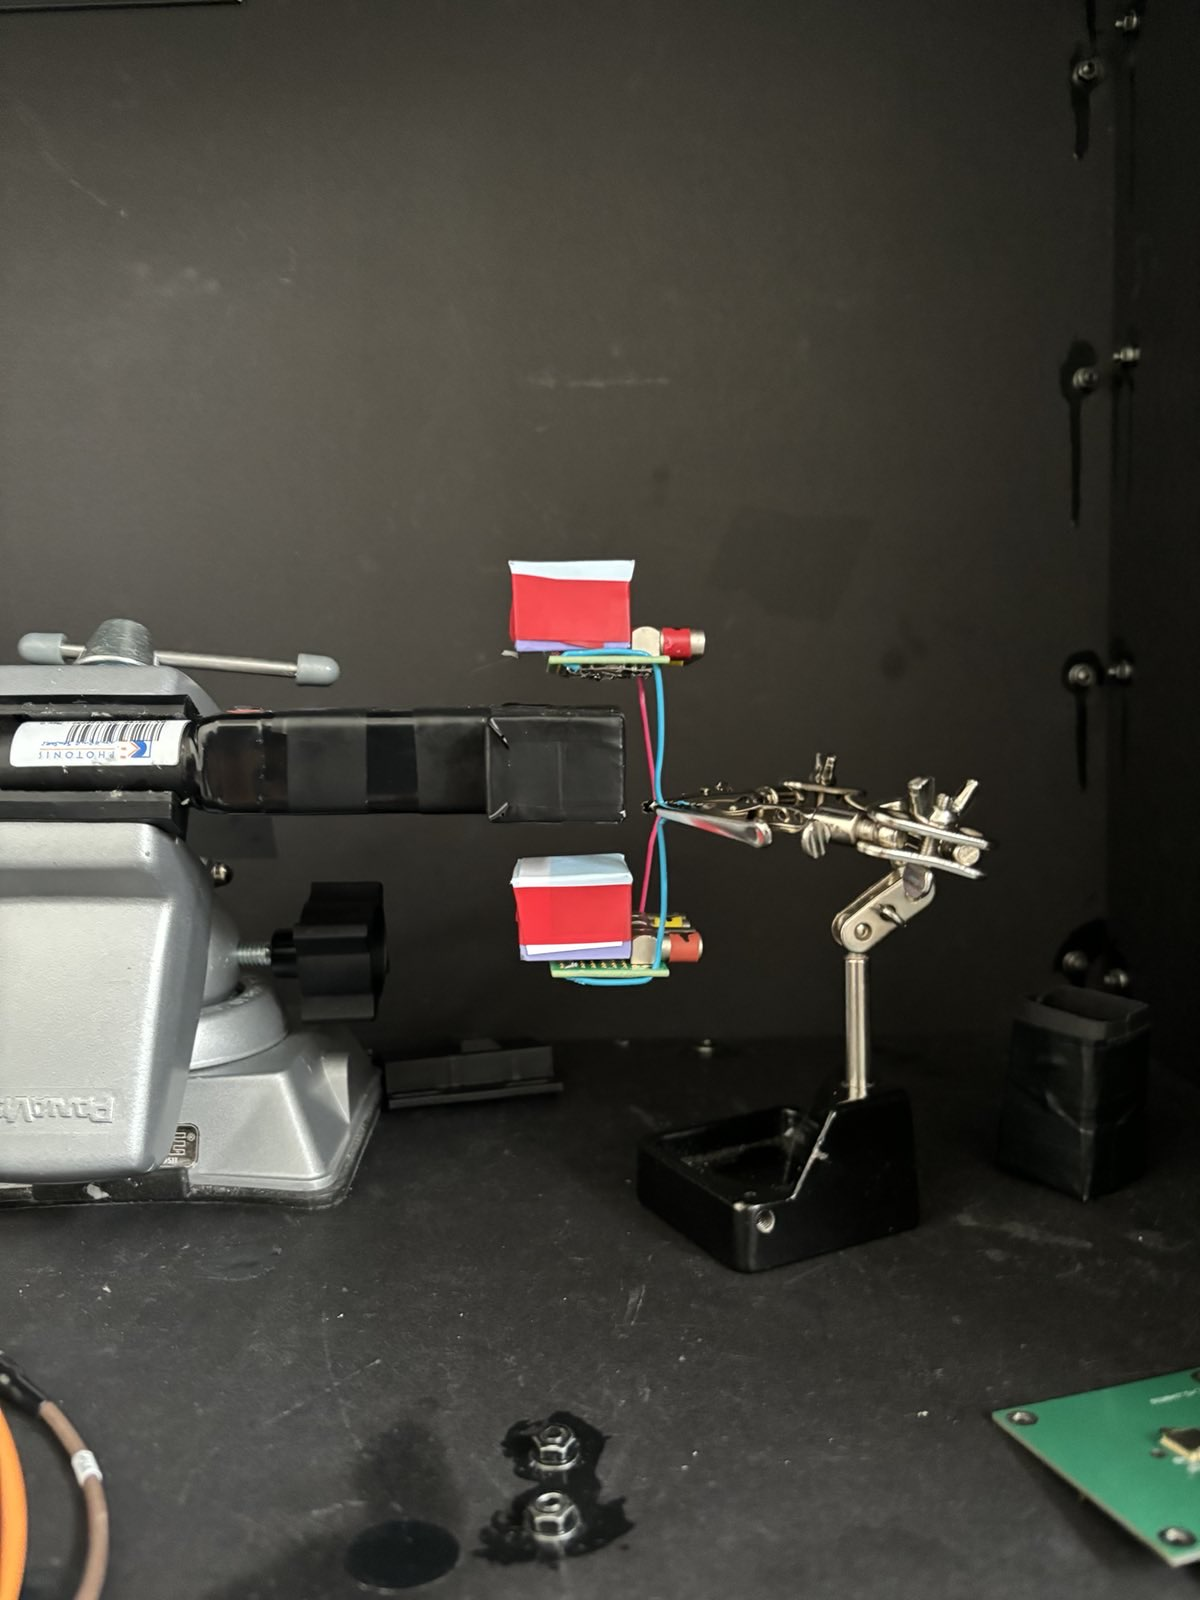
\includegraphics[trim=0 500 0 500, clip, width=0.8\textwidth, frame]{images/muon_telescope_setup.jpg}
            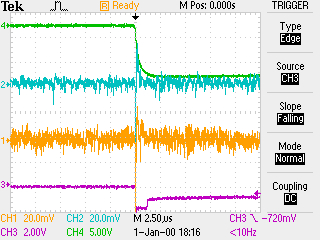
\includegraphics[width=0.6\textwidth, frame]{images/muon_coincidence_screenshot.jpg}
        \end{figure}
    \end{column}
    \begin{column}{0.5\textwidth}
        \begin{figure}
            \centering
            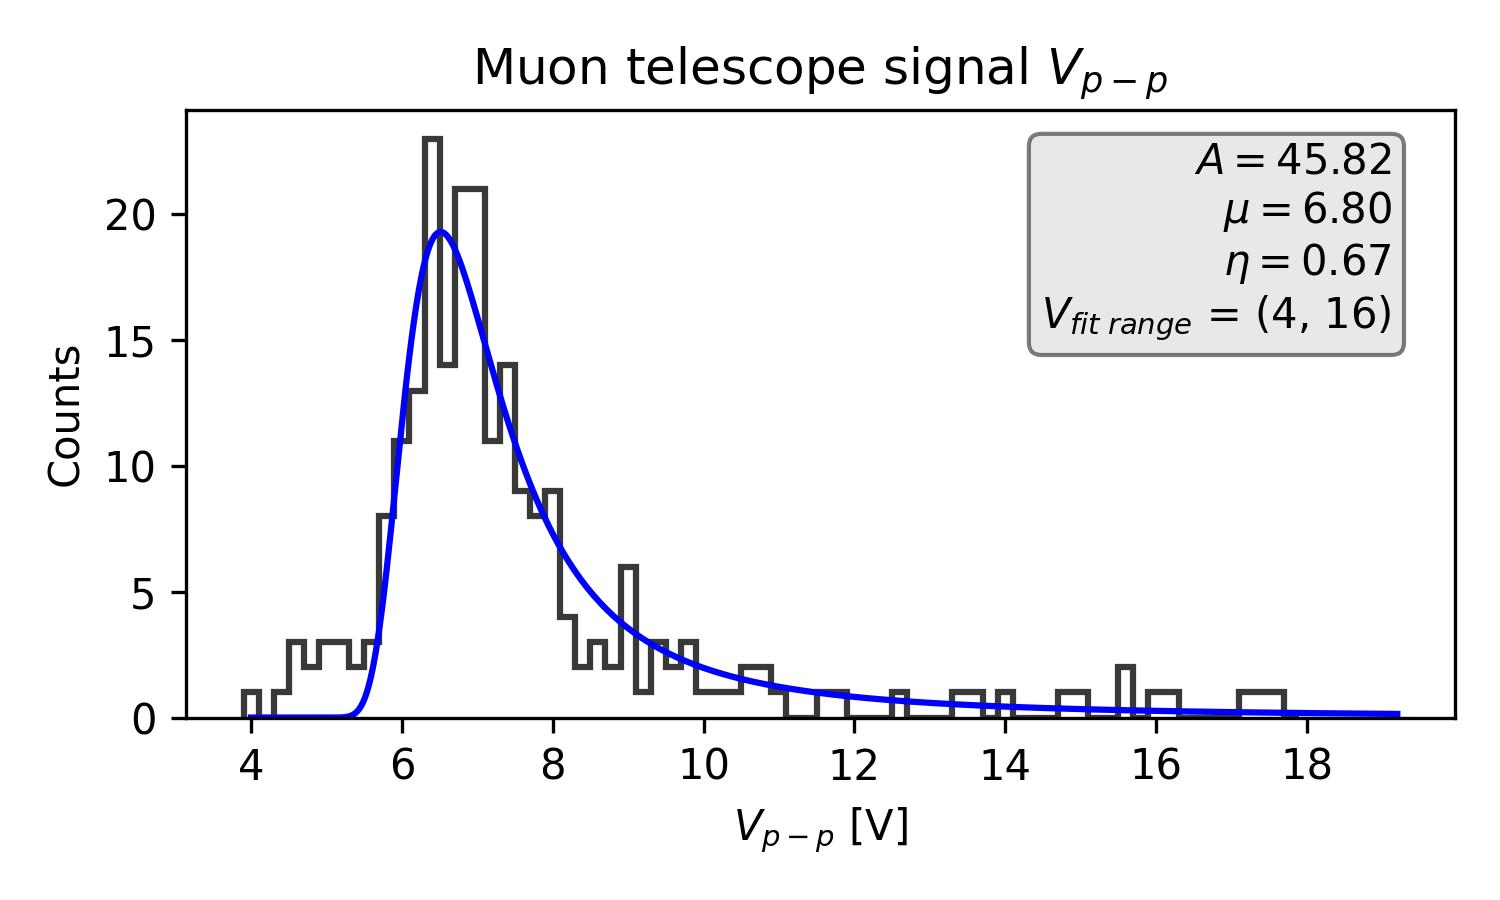
\includegraphics[width=0.8\textwidth, frame]{images/landau_fit.jpg}
        \end{figure}
        \begin{itemize}
            \item The telescope consists of two SiPM triggers and the BGO-PMT in the middle
            \item The landau distribution of the muon signal is apparent
        \end{itemize}
    \end{column}
\end{columnframe}

% \begin{columnframe}{}
%     \begin{column}{0.5\textwidth}
%     \end{column}
%     \begin{column}{0.5\textwidth}
%     \end{column}
% \end{columnframe}

% \setbeamertemplate{headline}{}
% \setbeamertemplate{footline}{}
\begin{frame}[plain]
    \centering
    \Large{Thank you for your attention}
    \vspace{0.5cm}

    \small{Questions?}
\end{frame}

\appendix

\begin{frame}{Signal height as a function of light attenuation}
    \begin{columns}
        \begin{column}{0.5\textwidth}
            \begin{figure}
                \centering
                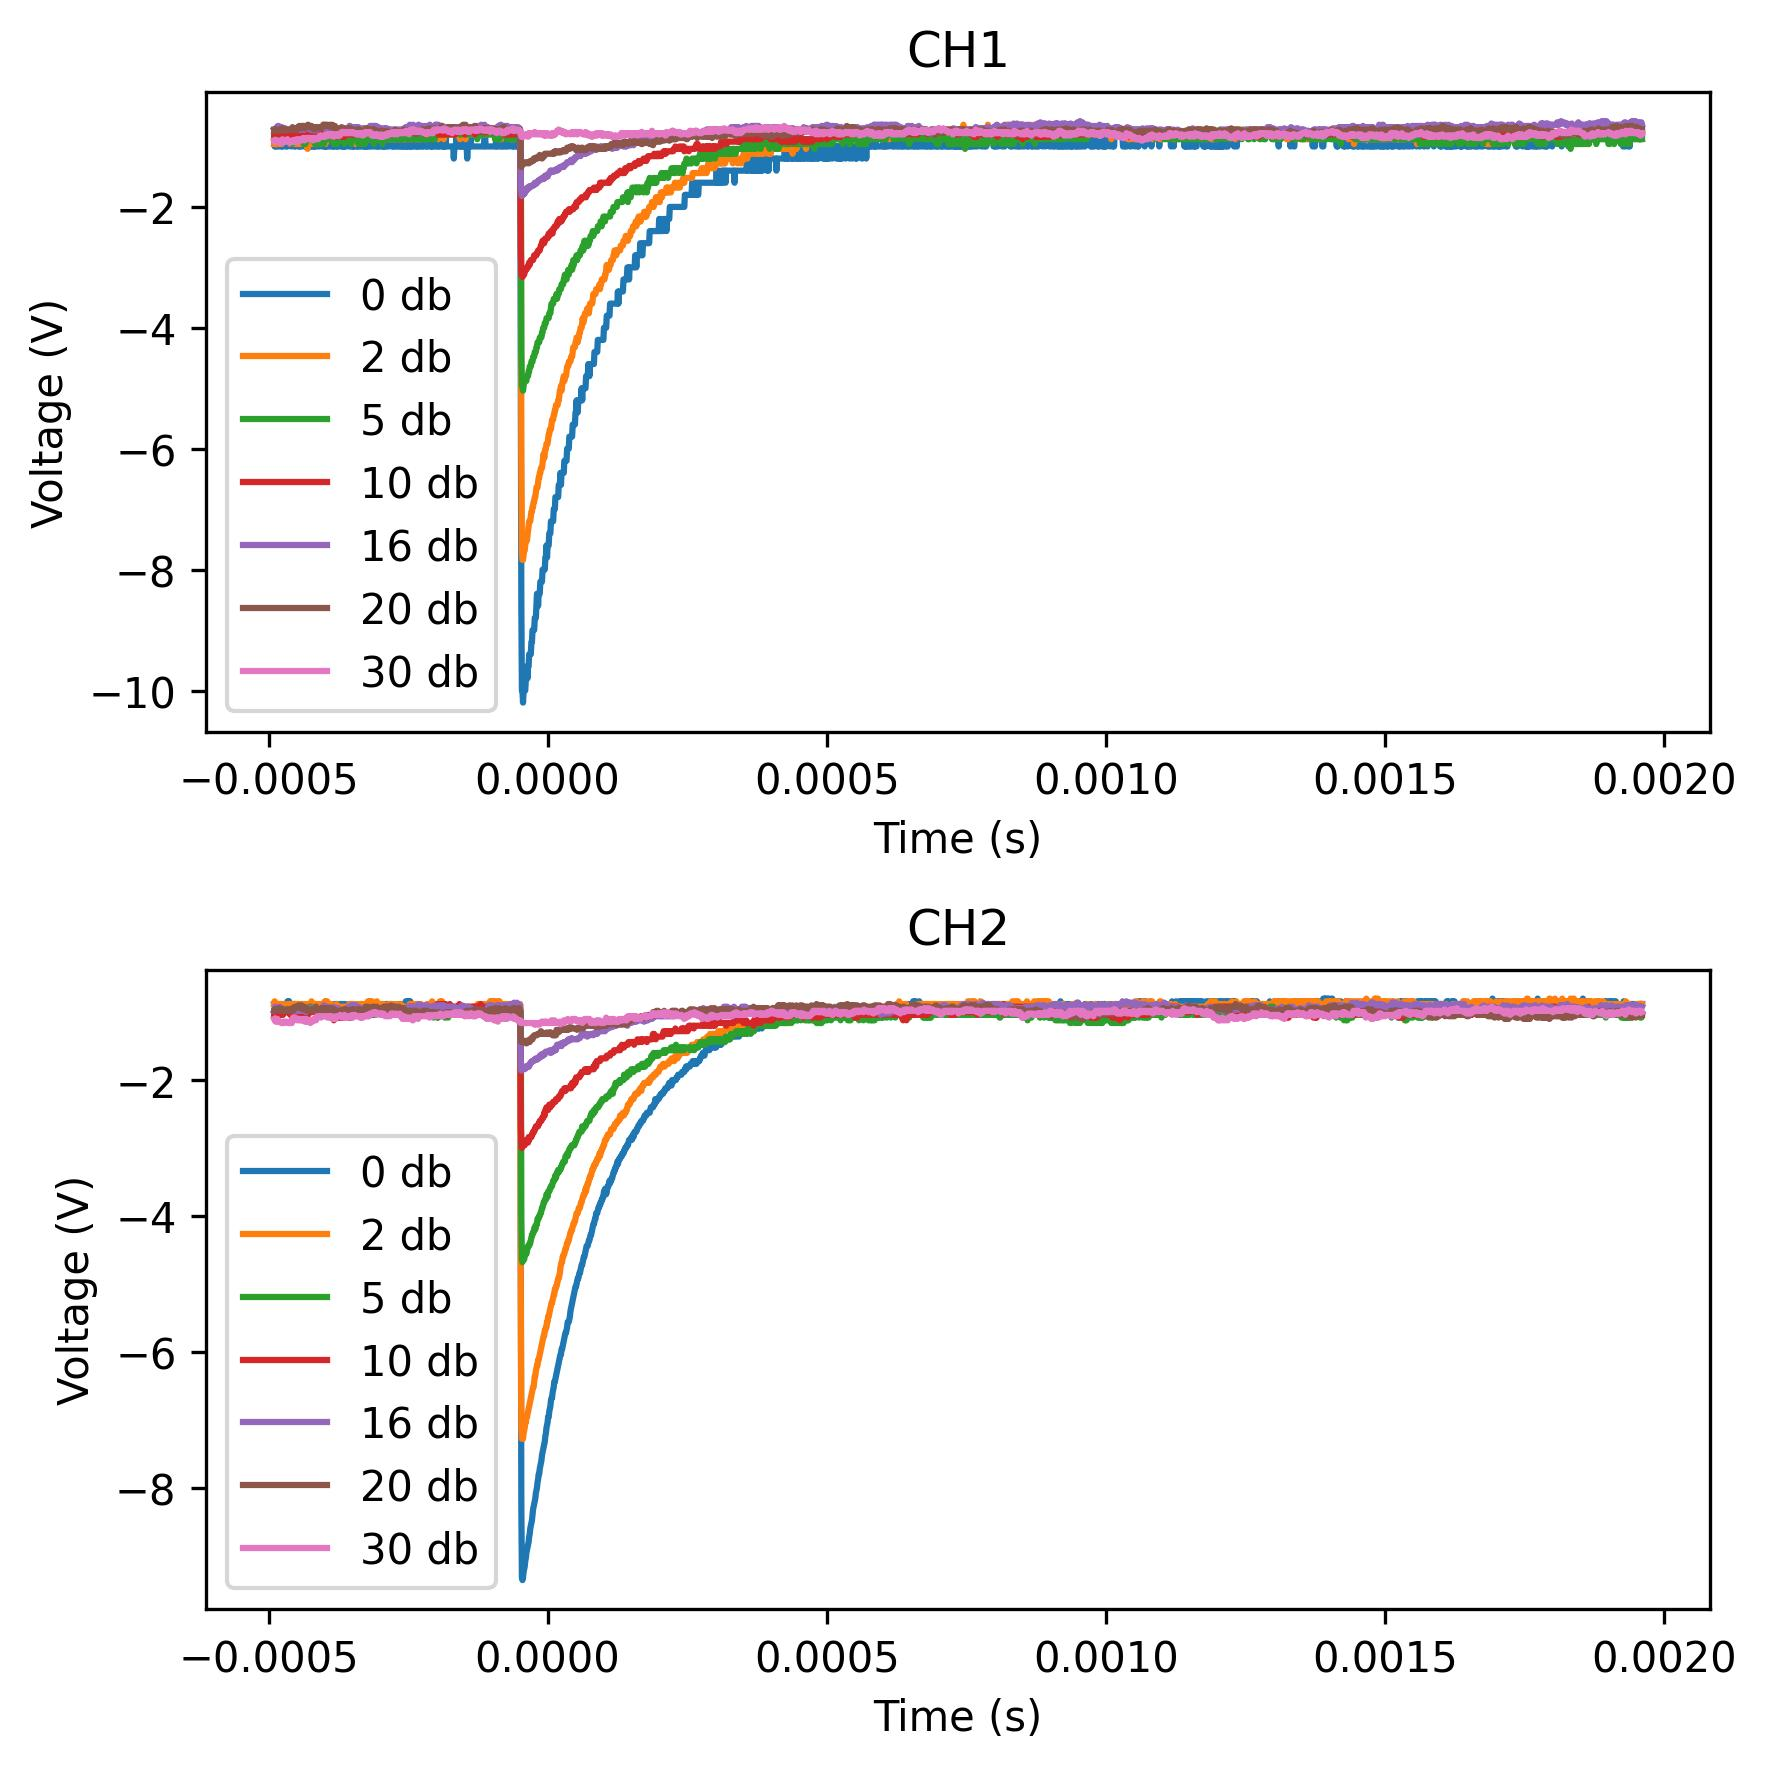
\includegraphics[width=0.8\textwidth, frame]{images/db_sigs_0_30.jpg}
            \end{figure}
        \end{column}
        \begin{column}{0.5\textwidth}
            \begin{figure}
                \centering
                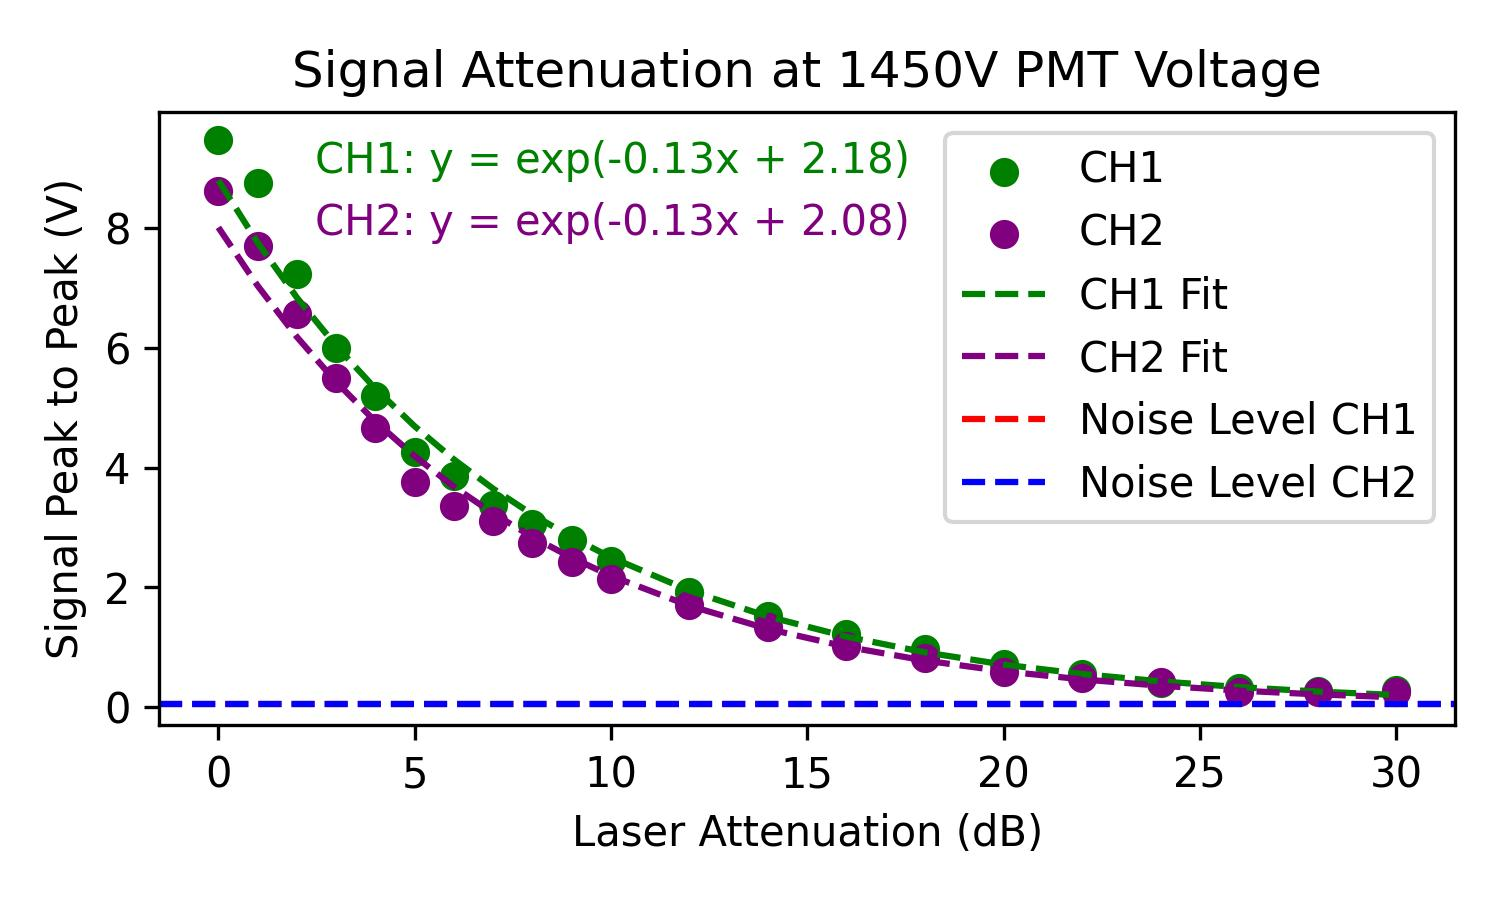
\includegraphics[width=0.8\textwidth, frame]{images/att_sig_exp_1450V_fit.jpg}
            \end{figure}
        \end{column}
    \end{columns}
\end{frame}

\begin{frame}{Single Photon Resolution}
    \begin{columns}
        \begin{column}{0.5\textwidth}
            \begin{figure}
                \centering
                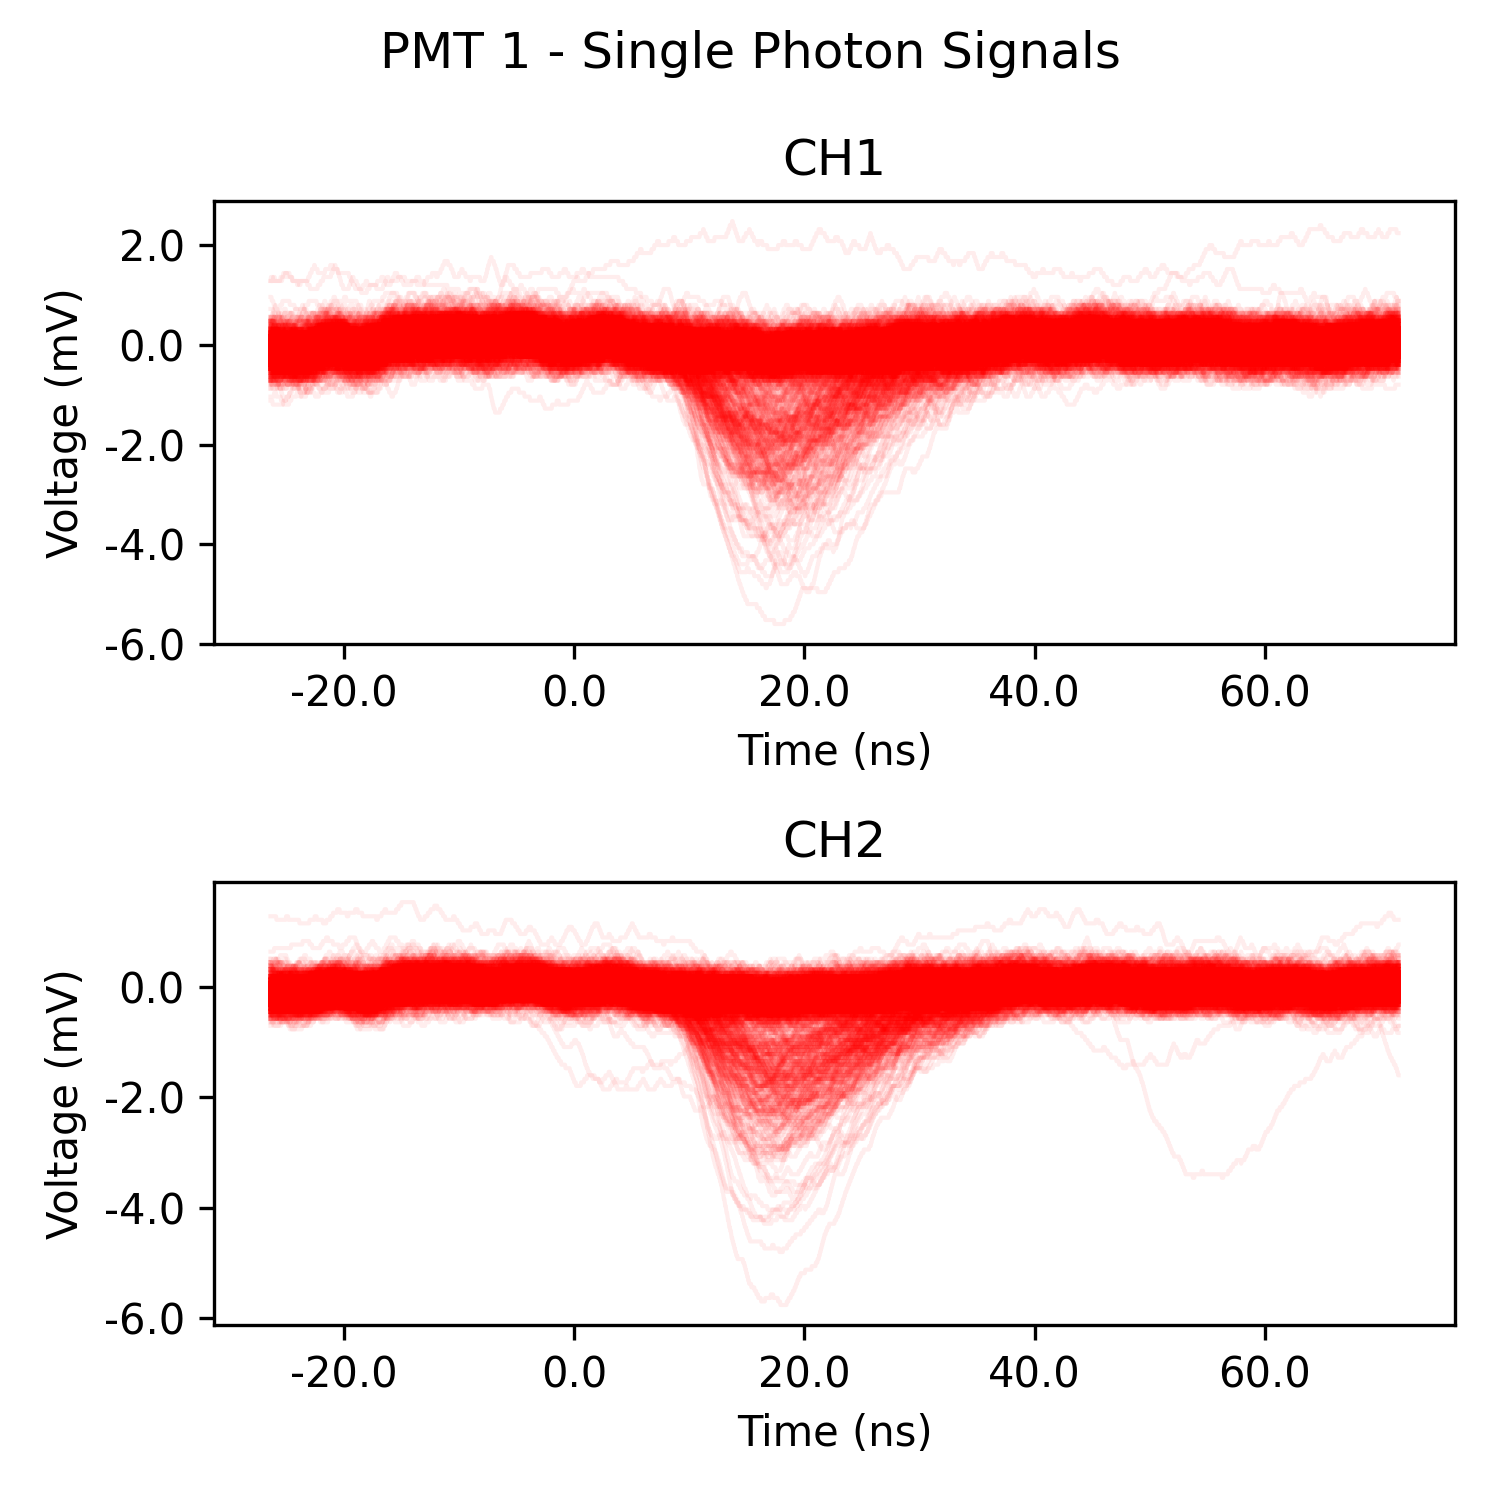
\includegraphics[width=0.8\textwidth, frame]{images/single_photon_signals.png}
            \end{figure}
        \end{column}
        \begin{column}{0.5\textwidth}
            \begin{figure}
                \centering
                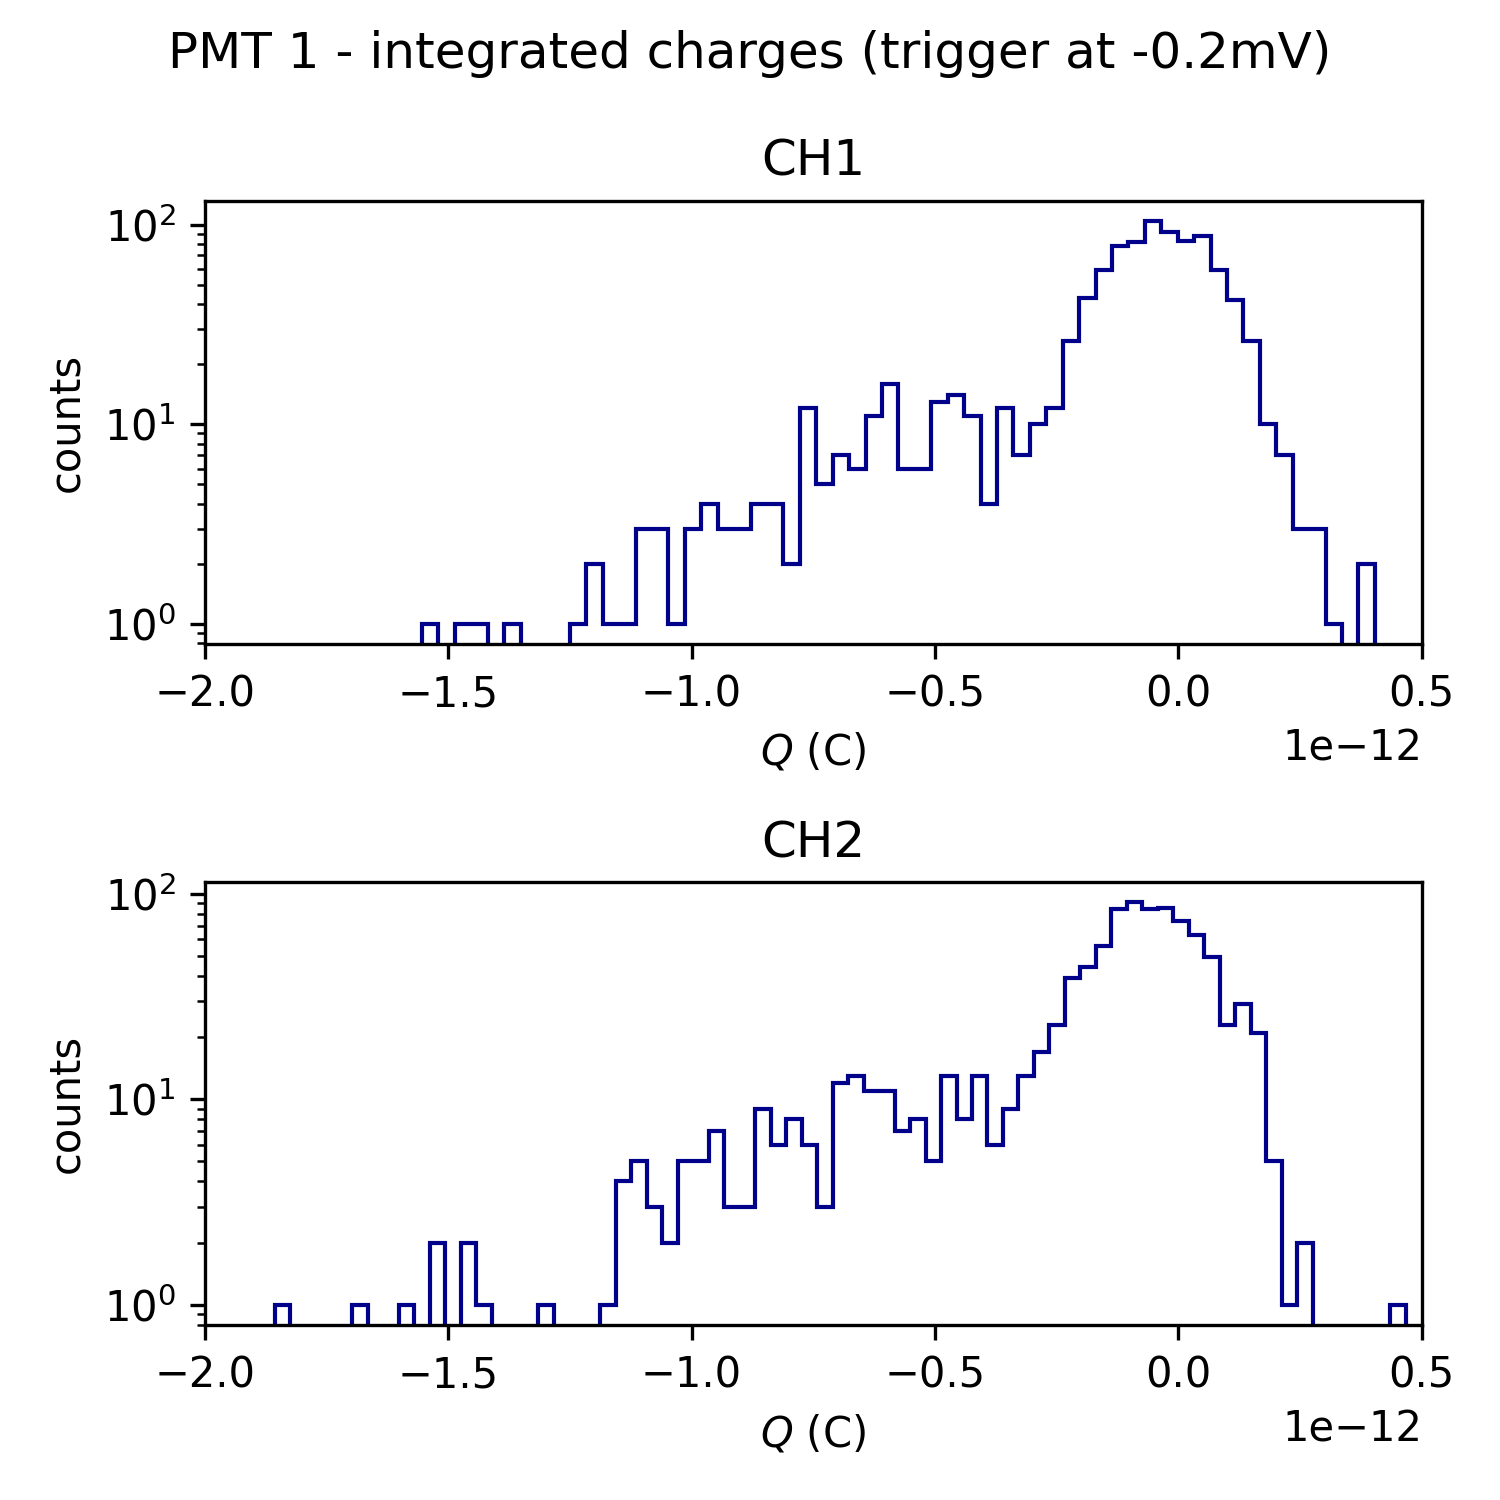
\includegraphics[width=0.8\textwidth, frame]{images/single_photon_integral_hist.png}
            \end{figure}
        \end{column}
    \end{columns}
\end{frame}


\end{document}